\documentclass[twoside, 12pt]{report}
\usepackage{graphicx} % Required for inserting images
\usepackage[utf8]{inputenc}
\usepackage{tikz}
\usepackage{pgfplots}
\usepackage{hyperref}
\usepackage{xcolor}
\usepackage[skip=8pt, indent=20pt]{parskip}
\usepackage[authoryear]{natbib}
\usepackage{setspace} \onehalfspacing
\usepackage{booktabs}
\usepackage{colortbl}
\usepackage{array}
\usepackage{xcolor}
\usepackage{amsmath}
\usepackage{cleveref}
\usepackage{annotate-equations}
\usepackage{float}
\usepackage{geometry}
\usepackage{color,soul}
\usepackage{appendix}
\usepackage{pdflscape}


% Set page margins
\geometry{
    letterpaper,
    inner=30mm,
    outer=20mm,
}


% Set graphics path
\graphicspath{{images/}}

% % Define colours
\definecolor{lightBlue}{RGB}{129, 183, 242}
\definecolor{lightGrey}{RGB}{128, 128, 128}
\definecolor{lightRed}{RGB}{255, 143, 143}
\definecolor{lightGreen}{RGB}{46, 184, 59}
\definecolor{lightPurple}{RGB}{160, 98, 239}
\definecolor{lightgray}{gray}{0.92}

% Set dark mode
% \pagecolor[rgb]{0,0,0} %black
% \color[rgb]{0.5,0.5,0.5} %grey

% Packages setup
\hypersetup{
    colorlinks,
    citecolor=darkgray,
    filecolor=darkgray,
    linkcolor=darkgray,
    urlcolor=darkgray
}

\usetikzlibrary{shapes.multipart, arrows.meta, decorations.markings}

\title{MASc Thesis}
\author{Andres Castillo}
\date{December 2023}

\raggedbottom

\begin{document}
\begin{sloppypar}

% \maketitle
\begin{titlepage}
    \begin{center}
        \vspace*{1cm}

        \Huge
        \textbf{Predicting salaries in the Greater Toronto Area: A Bayesian approach}

        \vspace{1.5cm}

        \Large
        by

        \vspace{1.5cm}

        \textbf{Andres Danilo Castillo Vega}

        \vfill

        A thesis submitted in conformity with the requirements\\
        for the degree of Master of Applied Science\\
        Department of Civil and Mineral Engineering\\
        University of Toronto

        \vspace{1.5cm}

        \Large
        \textcopyright \hspace{1pt} by Andres Danilo Castillo Vega 2023

        \vspace{0.8cm}

    \end{center}
\end{titlepage}

\chapter*{Abstract}
\begin{spacing}{2}
Labour markets and transportation systems are at the core of urban life. Attributes such as residential and work locations, household income, and auto ownership are closely related to the interactions in the labour market. Since salaries are a key component of these interactions, predicting salaries becomes an important task for integrating labour market outcomes into travel behaviour modelling. Using a data-driven approach, we estimate a Bayesian hierarchical model to predict salary distributions in the Greater Toronto Area. The results of this work demonstrate that this approach provides better estimates at both the aggregated and disaggregated levels and generates more robust predictions by producing probability distributions instead of point estimates. This characteristic is key for using this model in an urban simulation setting such as the ILUTE framework. 
\end{spacing}


\chapter*{Acknowledgements}
\vspace{-1cm}
The completion of this thesis marks the end of a long journey that began at least seven years ago as a dream. This journey has been full of learnings and experiences that define who I am. Today also marks the beginning of a new stage in my life. For that reason, I would like to thank all the people who have been part of this journey and made it possible.

To my love, Ale, for being my support and inspiration. I feel so fortunate to have you in my life. This achievement is also yours. To my love, Emi, you arrived in our lives at the perfect moment, and we are happily waiting for you. I hope someday you can find this work as an inspiration to follow your dreams and never give up. There are no limits if you work with love and dedication.

To Prof. Eric Miller, for his patience, guidance, and support during this journey. I am very grateful for the opportunity to work with you and learn from your experience.

To Prof. Matthew Roorda, for kindly agreeing to be the second reader of this thesis and providing his feedback. Also, to all my colleagues at the University of Toronto, I learned a lot from all of you. Thanks for the good times and memories.

To my family, for their encouragement during this journey. All of you are continuously teaching me about the important things in life. This thesis is dedicated to the memory of my mother, Lucinda, who always believed in me and inspired me to follow my dreams. I am sure you would be very proud of this achievement. All that I have done is thanks to you.

Last but not least, to my dog, Avena. This thesis is also yours because you stayed with me during the long hours of work and study. You do not know how much those afternoon walks helped me to clear my mind and keep going.


\tableofcontents
\listoffigures
\listoftables

\chapter{Introduction}

Transportation models have grown in complexity by including 
more details on travel behaviour. However, some demographic 
and socioeconomic variables are still considered exogenous 
factors, introducing uncertainty and reducing the model's 
effectiveness in forecasting future scenarios. Since work 
trips are the most frequent trips in urban areas, understanding 
work-related attributes is relevant for travel demand modelling. 
Some attributes such as the place of residence, place of work, 
household income, auto ownership, and mode choice can directly 
or indirectly relate to the labour market.

According to \citet{HarmonMiller2020}, the inclusion of labour 
market interactions within urban simulations has had little 
development despite the critical relationship between work and 
transportation systems in urban areas. In their paper, 
\citet{HarmonMiller2020} proposed an Agent-Based framework for 
simulating the demand and supply interactions of the labour 
market. This framework provided the first approach to a fully 
endogenous labour market simulation within a 
transportation-related model. Nevertheless, as discussed by 
\citet{Harmon2013}, much research still needs to be done to ensure 
the validity of results as the model evolves in time, to 
understand the interactions between agents, and to investigate 
the factors influencing the recruitment process within firms. 
In particular, He provides some evidence that the existent wage 
model could be underestimating salaries in the long run, which 
can be critical given the role of wages in the labour market. 
\\
\\
\\
Therefore, this thesis presents a model that predicts salary 
based on individual attributes of a worker using the principles 
of Bayesian inference. This model improves the prediction 
accuracy by accounting for the hierarchical structure of the 
data, which better simulates the variability in the salaries 
at both an aggregated and disaggregated level.

\section{Outline}

Although all sections in this document are structured 
sequentially, some can be optional according to the reader's 
knowledge of Bayesian inference. After this introduction, 
Chapter 2 presents an overview of economic theory and discusses 
the role of salaries and wages in the labour market interactions. 
Chapter 3 briefly introduces Bayesian inference, the framework 
for estimating the proposed model. Chapter 4 discusses the data 
sources and the hierarchy of labour data. Additionally, it 
presents the main results of the exploratory data analysis that 
guides the model specification. Then, Chapter 5 presents the 
details of the proposed salary model and the validation results 
with new data, followed by Chapter 6, which discusses the 
integration of this proposed model into the existing ILUTE 
framework. Finally, Chapter 7 compiles the principal results, 
and discusses the future work.
\chapter{Literature review}

This chapter provides a systemic perspective on the labour 
markets supported by the literature. It starts with a brief 
discussion of the economic theory that governs labour markets, 
followed by an overview of different implementations of 
microsimulation models with an emphasis on the ILUTE framework. 
Finally, this chapter closes with a discussion of the gaps 
that guide the work in the subsequent chapters. Although the 
economic literature on this subject is extensive, this section 
is mainly based on the concepts and ideas stated 
by 

\chapter{Bayesian inference: From point estimates to probability distributions }\label{chapter:bayesian_inference}

This section presents an overview of the concepts in Bayesian inference used for the model estimation in the following chapters. It starts with a brief comparison between the Frequentist and Bayesian approaches. Then, it presents the theoretical foundations of Bayesian statistics and how these principles are transformed into a practical framework for parameter inference and modelling in the real world. 

This chapter is based on the ideas discussed by \citep{Lambert2018}, \citep{McElreath2016}, and \citep{Gelman2013} but is not intended to be an extensive review of the concepts. For further details, these sources are a good starting point. 

\section{The Bayesian paradigm: Frequentist vs Bayesian} 

Statistical inference has two “Schools of thought”: the Frequentist (or Classical) and the Bayesian approach. For frequentists, the data are assumed to be the result of an infinite number of repeated experiments with the same characteristics.  Then, the data are randomly sampled from a fixed and defined population, and any source of variation comes from that sampling process. Under this perspective, model parameters are assumed to be fixed but unknown values related to the population of interest, and the objective of inference is to calculate the best point estimate of the true value of the parameters given a data sample. 

In contrast, Bayesian statistics assume that data are observed and fixed quantities, and the source of variation comes from the uncertainty over the parameters. From this perspective, parameters are probabilistic values, and the objective of inference is to estimate the probability distribution of the model's parameters. Then, we use the data as evidence to update any prior belief about the underlying process. 

The debate about which approach is the best is exciting but long and almost philosophical; therefore, it is outside the scope of this document. However, as \citep{McElreath2016} points out, the Frequentist approach could make sense if the process of interest can be replicated multiple times, as in the case of many natural sciences (i.e., multiple controlled experiments in a laboratory). In contexts where the data collection can only be performed once, such as in many social sciences (i.e., democratic elections, population census), a Bayesian approach could be more aligned with the data nature. 

A quick overview of the Bayesian thinking framework is presented in \Cref{eq:bayesian_paradigm} \citep{Lambert2018}. The procedure begins with establishing prior beliefs about the process under analysis. Then, evidence (data) is gathered to update the prior beliefs using the model. The update is known as the posterior belief that includes the knowledge from both the priors and the data. 

\begin{equation}\label{eq:bayesian_paradigm}
    \text{prior} + \text{data} \xrightarrow{\ \ \ \ model\ \ \ \ } \text{posterior}
\end{equation}

\section{The basics of Bayesian inference} 

As the aim of statistical inference is to estimate the parameters of a model that recreates the process of interest, one of the objectives is to calculate the probability of getting the true parameters given the observed data or $P(\theta|data)$. However, as the true parameters are unknown, only the likelihood of the data being generated by the model parameters $P(data|\theta)$ can be calculated. 

According to\citet{Lambert2018}, both Frequentist and Bayesian inference aim to go from $P(data|\theta)$ to $P(\theta|data)$. While in the frequentist perspective, this transformation is not correctly carried out\footnote{The estimation is done by selecting the parameters that maximize the likelihood of obtaining our observed data.}, the Bayesian perspective applies the Bayes rule --\Cref{eq:bayes_rule}-- to properly transform the likelihood into a probability $P(data|\theta)\rightarrow P(\theta|data)$. The details of this transformation are reviewed in the following sections.

\vspace{3em}
\renewcommand{\eqnhighlightheight}{\vphantom{\hat{H}}\mathstrut}
\begin{equation}\label{eq:bayes_rule}
    \eqnmarkbox[lightBlue]{posterior}{P(\theta|data)} = \frac{\eqnmarkbox[lightGreen]{likelihood}{P(data|\theta)}\cdot\eqnmarkbox[lightRed]{prior}{P(\theta)}}{\eqnmarkbox[lightPurple]{evidence}{P(data)}}
\end{equation}
\annotate[yshift=2em]{above,left}{posterior}{posterior}
\annotate[yshift=2em]{above}{likelihood}{likelihood}
\annotate[yshift=1em]{above}{prior}{prior}
\annotate[yshift=-1em]{below}{evidence}{evidence}
\vspace{2em}

\subsection{Likelihood} 

One of the most important tasks when performing statistical inference is the choice of the model and its parameters. As the parameters are unknown to the modeller, the inference task is to estimate their value. One approach is to test different parameters on the chosen model and calculate the probability of getting the observed data for each set of values. The function that describes these probabilities corresponds to the \textit{likelihood function}. However, as this function is not a probability distribution, Bayesian statistics use Bayes theorem to convert this likelihood into a proper probability distribution. 

When defining the model, intrinsically, the data generation process is considered. Therefore, the likelihood includes the evidence and all the assumptions about the process. The higher the likelihood\footnote{In practice, the likelihood is transformed into the log-likelihood to ease the computation. This transformation also modifies the optimization process into a minimization. However, both approaches yield the same results.}, the better the estimation of our true parameter distributions. Given the directionality of the Bayesian thinking process $prior+data\rightarrow posterior$, the model definition is one of the most important factors in Bayesian inference. If the model choice does not represent the data generation process, no matter the prior selection, the inference process will fail to produce parameters that represent the reality. 

\subsection{Prior }

Also known as prior belief, it is the distribution or group of distributions\footnote{There is one prior for each model parameter.} representing previous knowledge of the process under study. This distribution encodes the existing knowledge and the modeller's uncertainty of the model parameters. 

In some cases, the problem is widely studied, and there is enough evidence about the possible values of the model parameters. In other cases, there is no previous evidence about the process. In the former case, the modeller is more confident about the expected value of the model parameter and can approximate the shape and location of the probability distribution for the model parameters. In the latter case, the modeller is more uncertain about the possible parameter values, and a conservative approach is the best choice. Then, the prior choice represents the modeller's current knowledge of the process under study.

The prior selection is subjective as the current knowledge state can vary from one modeller to another. \citet{McElreath2016} argues that all modelling approaches, Frequentist and Bayesian, involve a certain degree of subjectivity. However, the Bayesian approach makes it explicit and open to scrutiny. If the current belief contradicts the evidence, the modeller can use the Bayes theorem to include this new evidence and update their prior belief. 

Prior distributions are classified by the knowledge state, as shown in \Cref{fig:priors}(a). \textit{Highly informative priors} are concentrated around a value, and \textit{non-informative priors} are widely distributed and assume almost equal probabilities given the uncertainty level. Likewise, the shape and distribution type choices are crucial for correct prior selection. \Cref{fig:priors}(b) shows some highly informative prior alternatives for modelling continuous and positive variables. When modelling processes with random components or in models that include linear predictors (e.g., linear regression, logistic regression), the parameters are usually represented by the normally distributed prior. This prior provides more information than the uniform but is more flexible to be updated in the process. These distributions are also known as \textit{weakly-informative priors}. 

\begin{figure}[h]
    \centering
    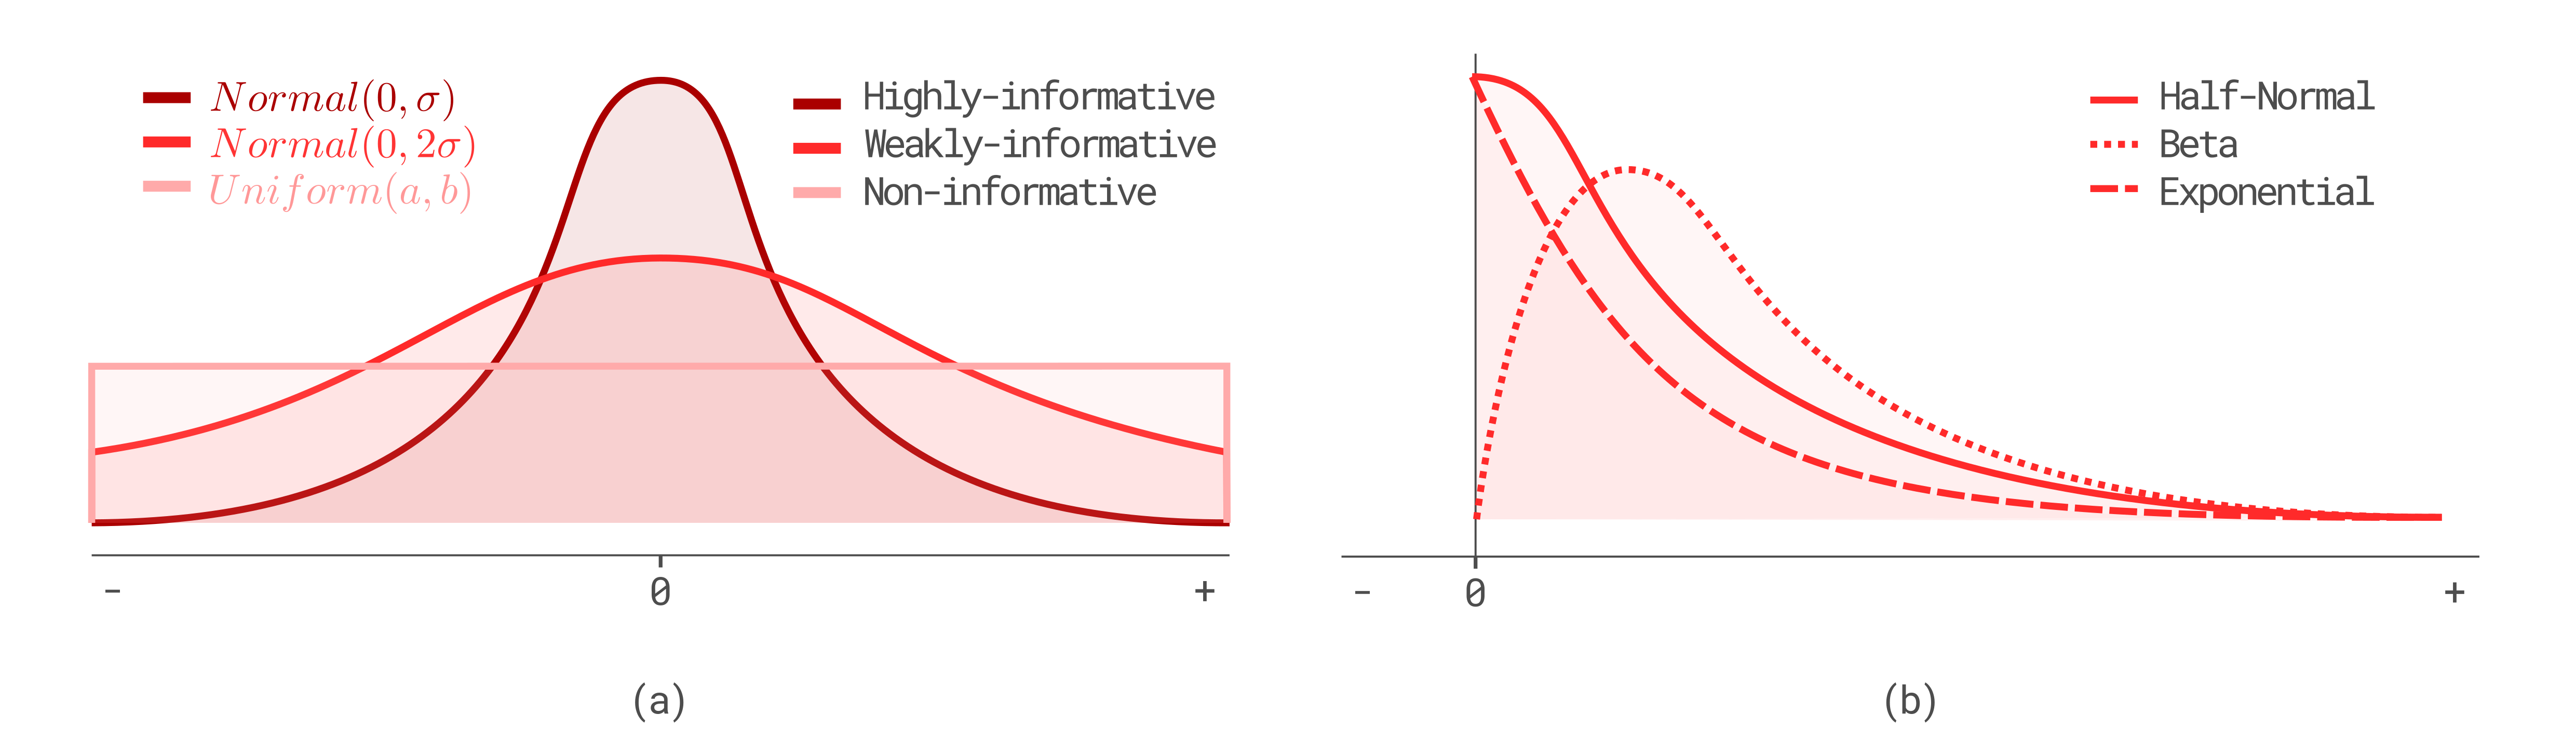
\includegraphics[width=1.0\textwidth]{images/ch3_informative_priors/informative_priors.png}
    \caption{Types of priors}
    \label{fig:priors}
\end{figure}

\subsection{Evidence} 

Also known as \textit{marginal likelihood}, it represents the probability of observing the data considering all possible parameter values. It is called marginal likelihood because it corresponds to the marginal probability calculated as the integral of the joint probability $P(data|\theta)$ across all $\theta$'s, as represented in \Cref{eq:marginal_likelihood}\citep{Lambert2018}. 

\begin{align}\label{eq:marginal_likelihood}
\begin{split}
    P(data)&=\int_{all \theta} P(data|\theta)\cdot P(\theta)d\theta  \\ 
    &=\int_{all \theta} P(data, \theta)d\theta
\end{split}
\end{align}

Although \Cref{eq:marginal_likelihood} is the formal definition, the marginal likelihood has an additional interpretation. Given that the likelihood function is not a probability distribution, it is expected that the multiplication of the likelihood by the prior is not either. Therefore, as the posterior needs to be a probability distribution, the marginal likelihood is the normalization factor that scales the numerator, so the area under the posterior distribution sums up to 1. Under this interpretation, the numerator in the Bayes theorem provides the shape of the posterior, while the Marginal Likelihood scales it out\footnote{This abstraction is key to introduce the sampling methods reviewed in \Cref{section:MCMC}}. 

The calculation of \Cref{eq:marginal_likelihood} can be trivial for simple models, but it becomes intractable for some real problems that include several parameters. This is one of the reasons why most of the Bayesian inference must be addressed using sampling methods instead of exact calculation. This will be reviewed in more detail in \Cref{section:MCMC}

\subsection{Posterior} 

Finally, applying the Bayes theorem to update the priors based on the evidence results in the posterior distribution. The posterior represents the updated probability distribution of our model's parameters and consolidates the knowledge of our system that was extracted from the data and the priors. 

While the Frequentist approach produces a point estimate for each parameter in the model, the Bayesian approach produces a probability distribution for each parameter, representing the uncertainty over the estimated model parameters. Then, point estimates such as mean, median, mode, and interval estimates can be calculated from this distribution. 

Although the point estimates produced by Frequentist and Bayesian approaches can be similar, there is a difference in the interval estimates produced by both approaches. In the Frequentist approach, the confidence interval (CI) is an interval of plausible values of a population parameter with a certain level of confidence constructed over many repeated experiments \citep{Devore2016}. For instance, a 95\% confidence level implies that if an experiment is repeated many times, 95\% of the samples will produce a CI that contains the true population parameter. Therefore, the confidence interval is a measure of the uncertainty over the interval, not over the parameter estimation \citep{Lambert2018}. 

In the Bayesian counterpart, the credible interval is a range that contains the true value of a population parameter with a particular probability. For instance, a 95\% credible interval means that the given range contains the true value with a probability of 95\%. Conversely to the Frequentist counterpart, the credible interval is a measure of the uncertainty over the estimation parameter. This interpretation of interval estimates seems more intuitive than the Frequentist confidence interval because it provides a probability over the parameters of interest. 

\section{Applying Bayes theorem: Markov Chain Monte Carlo sampling }\label{section:MCMC}

As discussed in the last section, the calculation of the denominator in the Bayes theorem complicates the application of Bayesian inference to real problems. The solution is to abandon the idea of exact calculation and use alternative methods to estimate the posterior distribution. One approach is to sample from the distribution to build an approximation; however, the posterior is still unknown until we can solve the denominator. 

Coming back to the idea that the numerator of the Bayes theorem provides the shape of our posterior and the denominator is a scaling factor, we can rewrite the Bayes theorem as: 


\begin{align}\label{eq:bayes_numerator}
\begin{split}
    P(\theta|data)&=\frac{P(data|\theta)\cdot P(\theta)}{P(data)}\\
    P(\theta|data) & \propto P(data|\theta)\cdot P(\theta)\\
\end{split}
\end{align}

In \Cref{eq:bayes_numerator}, the posterior is proportional to the multiplication of the likelihood function and the prior. Given that both terms in the numerator are known\footnote{Priors are defined by the modeller and likelihood is calculated based on the model choice and the observed data}, it is possible to sample from this function even if the denominator is unknown (it is not normalized), as shown in \Cref{fig:scalling_posterior}. 

\begin{figure}[H]
    \centering
    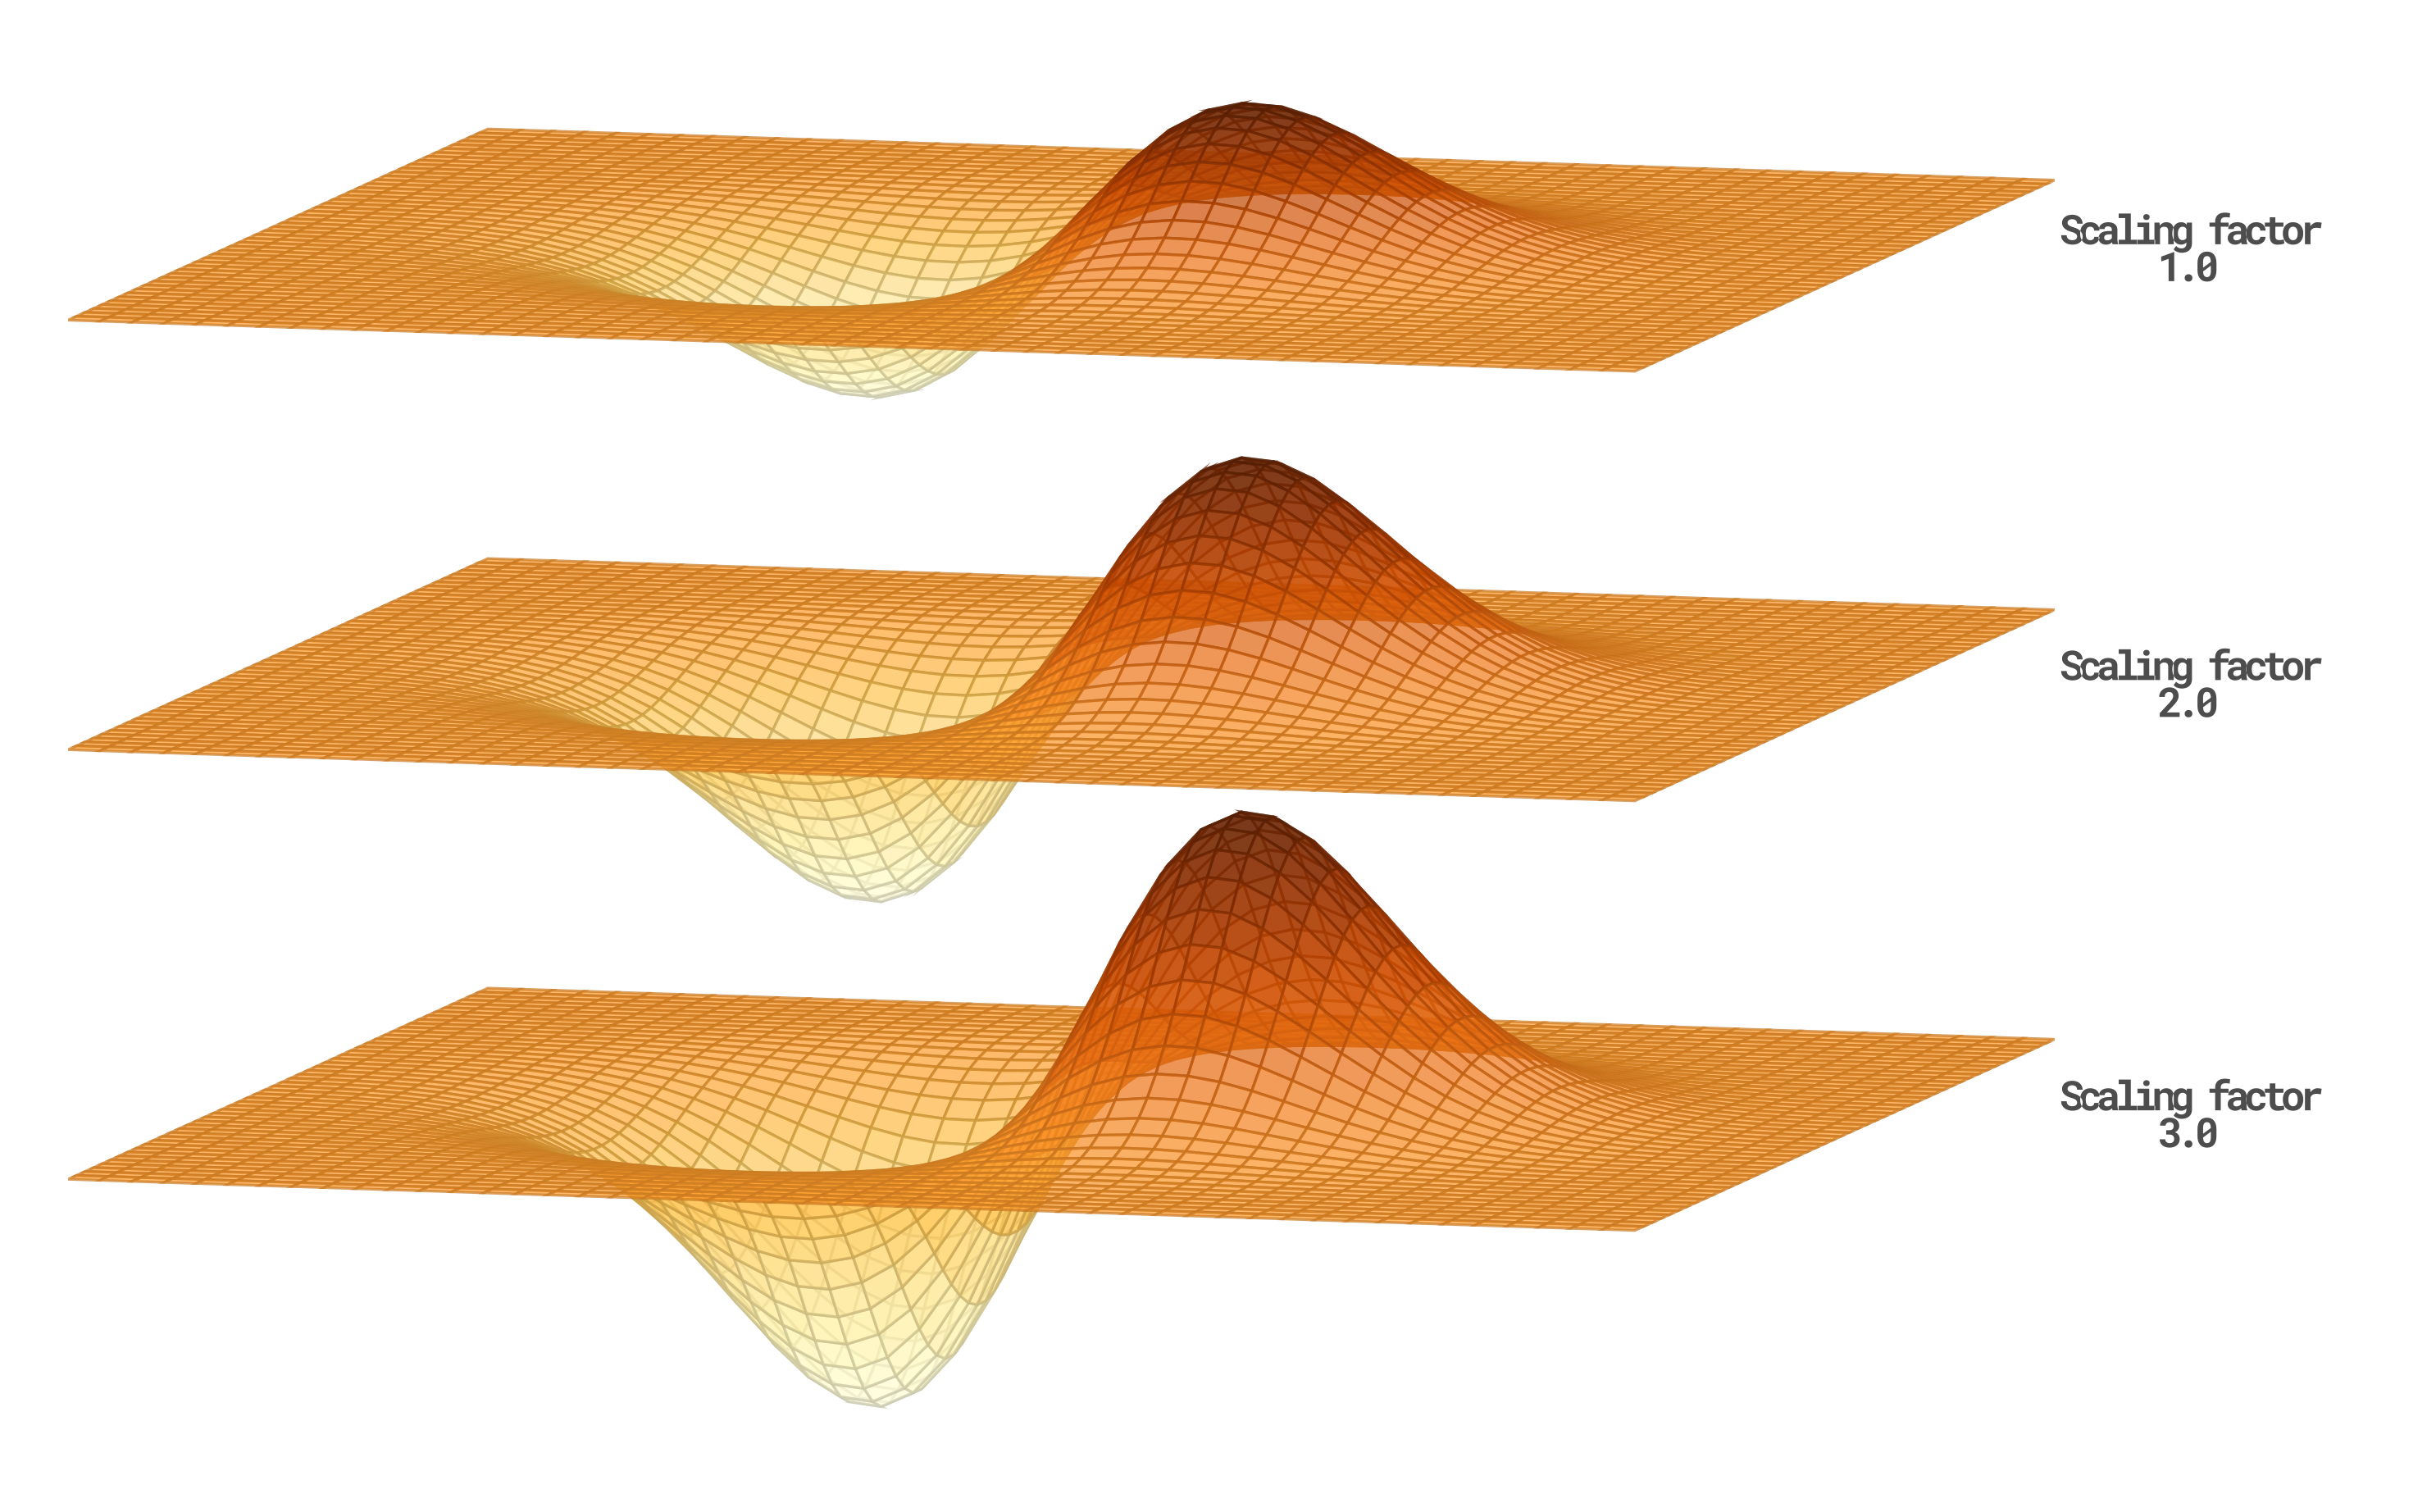
\includegraphics[width=1.0\textwidth]{images/ch3_scaling_posterior_space/scaling_posterior.png}
    \caption{Effect of scaling factor in the posterior space}
    \label{fig:scalling_posterior}
\end{figure}

This sampling process uses a method known as Markov Chain Monte Carlo (MCMC), which allows the approximation of a probability distribution by obtaining a sequence of random samples. The following section briefly introduces one algorithm within the MCMC family called Hamiltonian Monte Carlo (HMC), which is used in the development of this thesis. For further details of this algorithm, please review \citep{Lambert2018} and \citep{Neal2012}.

\subsection{Sampling from posterior: Hamiltonian Monte Carlo }

As the objective of the sampling process is to approximate the shape of the posterior distribution in \Cref{eq:bayes_numerator} (also known as \textit{posterior space}), different approaches such as rejection sampling, Gibbs sampling, or a simple Random Walk sampling can be used. However, these techniques are inefficient because they do not consider the shape of the distribution\footnote{An efficient sampler produces more samples from areas in which the posterior peaks (high probability density) and fewer samples from the rest of the distribution.}. 

The \textit{Hamiltonian Monte Carlo} method (HMC), a special case within the family of Markov Chain Monte Carlo (MCMC) algorithms, explores the posterior space more efficiently by using an analogy of a physical system in which a frictionless particle is moving around this space. In this physical system, two forces interact with the particle: gravity and the initial random momentum\footnote{This is the initial random impulse the particle receives that allows it to explore the posterior space.}. As the system is frictionless, the particle's position can be obtained at any time based on the previous position and the momentum applied to the particle \citep{Gelman2013,Lambert2018,McElreath2016,Neal2012}. 

To begin with, the posterior space is transformed into the negative log of the posterior $-log[(P(data|\theta))\cdot P(\theta)]$, also known as NLP space. This transformation converts all the peaks in the posterior space (zones with higher probability density) into valleys and the valleys in the posterior space (zones with lower probability density) into peaks. The idea behind this transformation is that the particle will visit more often the valleys of the NLP space because of the gravity effect. Therefore, more samples are taken from the zones with high probability density in the posterior space. \Cref{fig:nlp_space} shows a representation of the posterior and NLP space. It is important to highlight that the dimension of the NLP space is equal to the number of parameters in our model. So, the coordinates in this space are the model parameters. 

\begin{figure}[H]
    \centering
    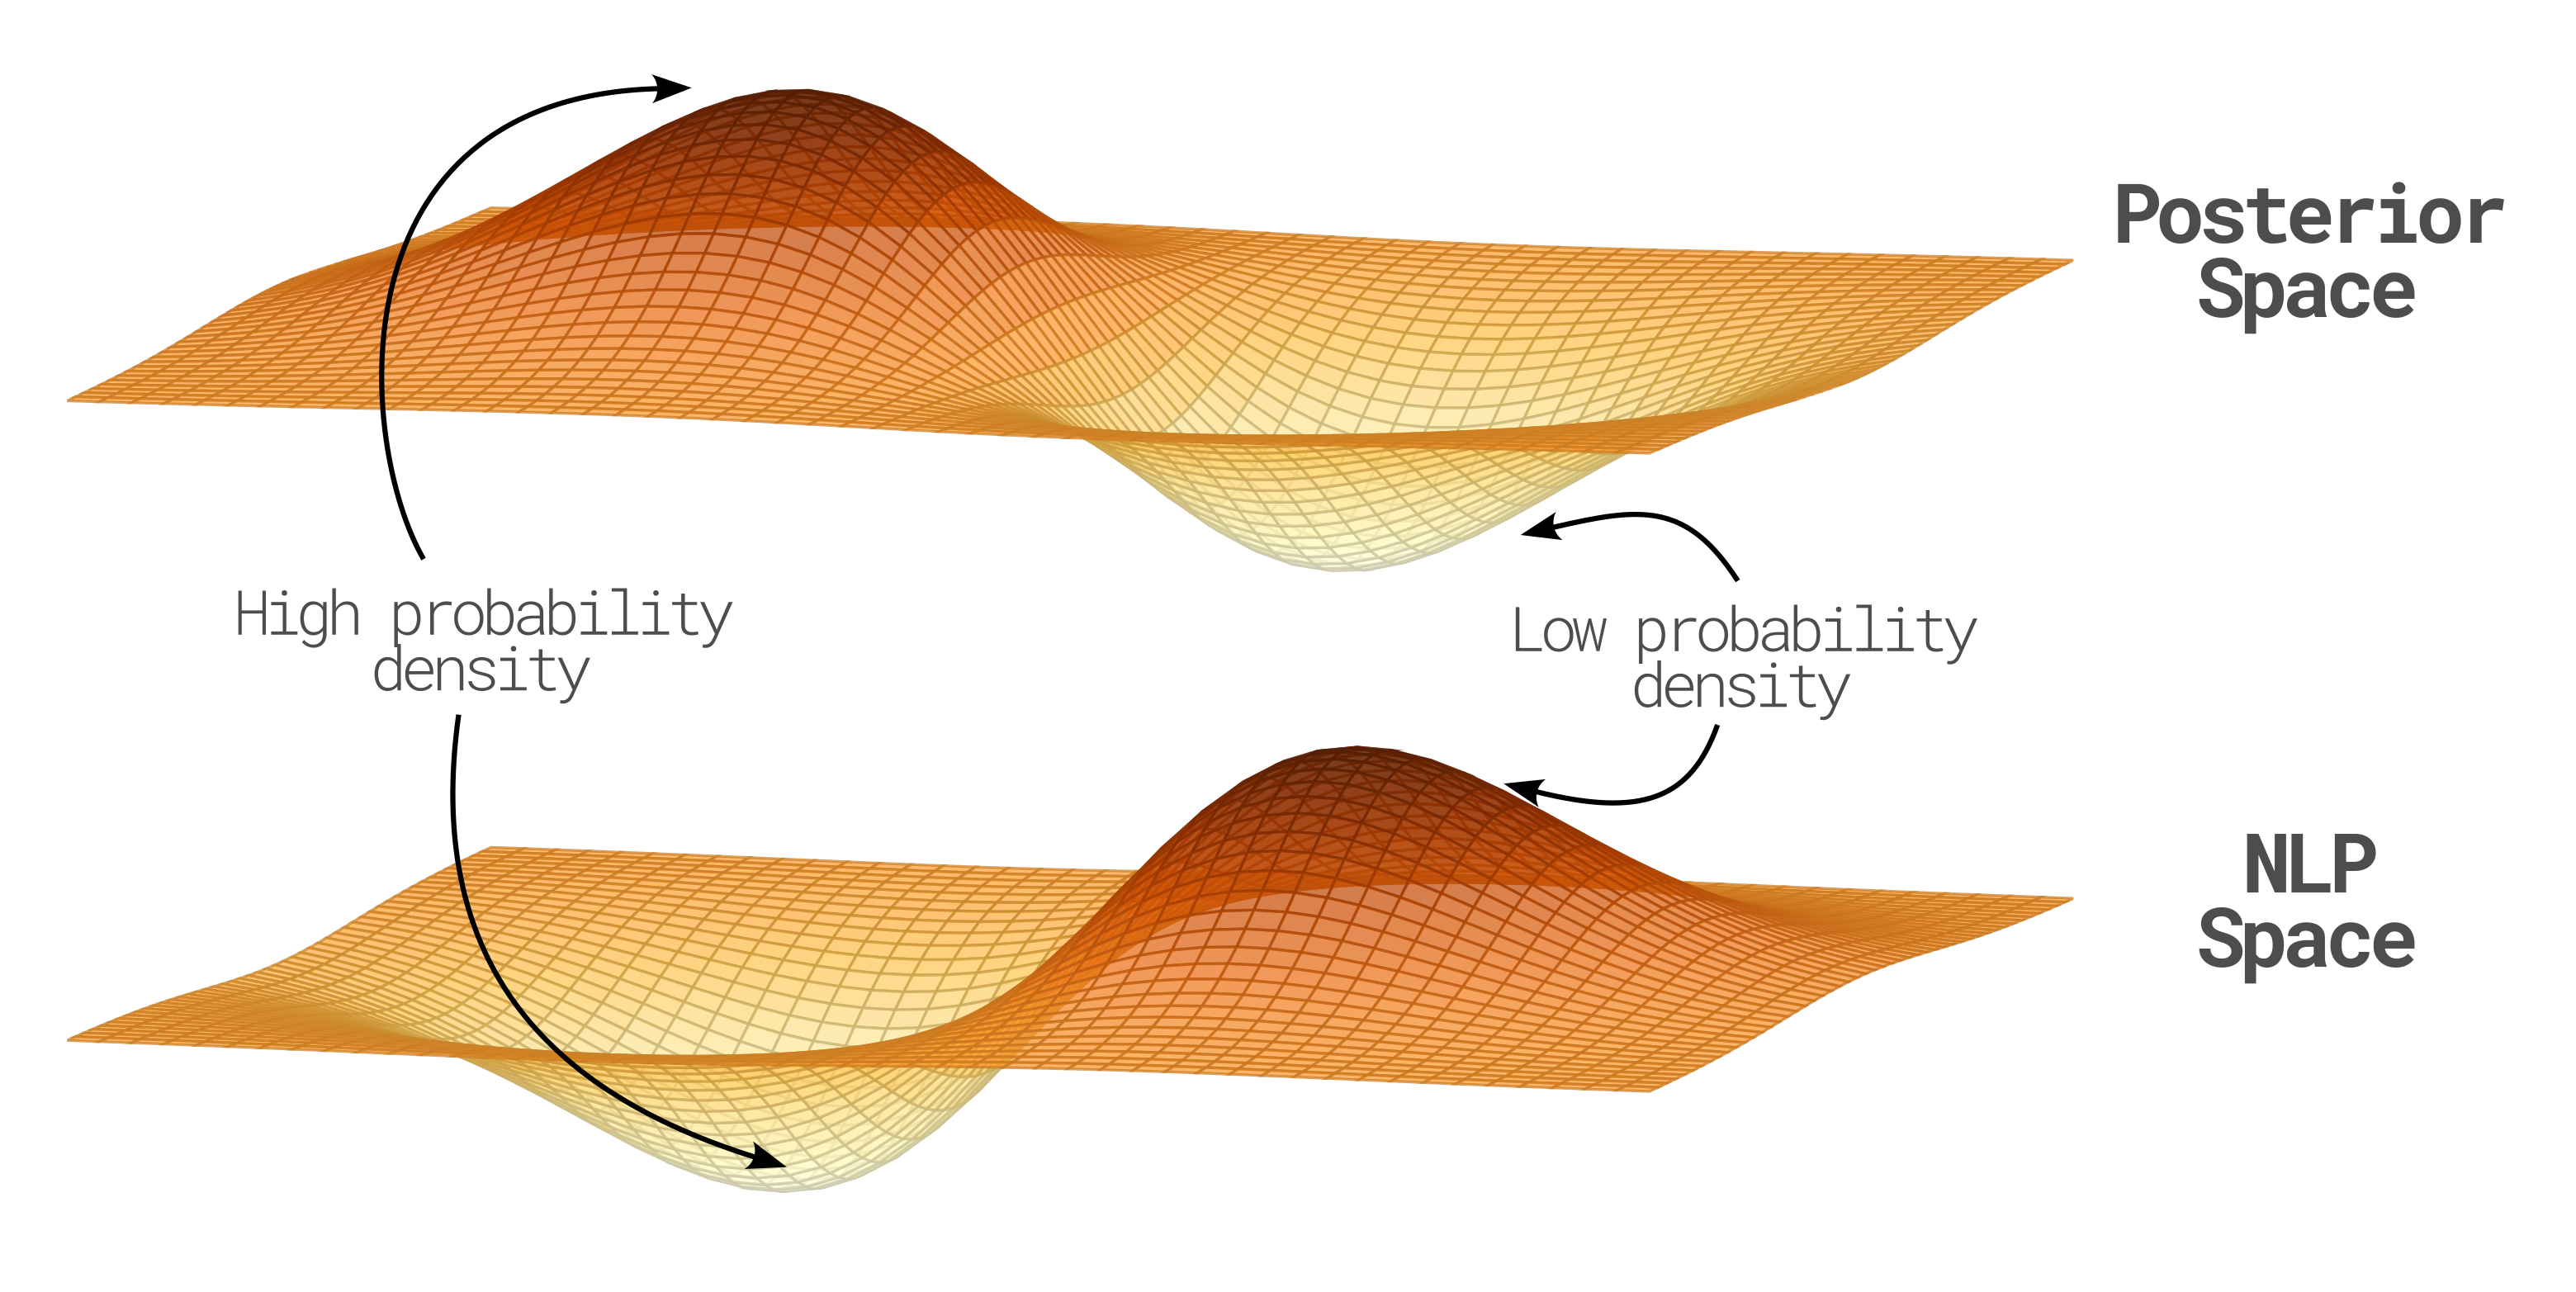
\includegraphics[width=1.0\textwidth]{images/ch3_NLP_space/nlp_space.png}
    \caption{Sampling from the posterior distribution and the NLP space }
    \label{fig:nlp_space}
\end{figure}

After this transformation, the initial position of the particle ${\theta_{o}}$ is randomly initialized\footnote{${\theta_{o}}$ is a vector of coordinates in the posterior space} and the following iterative process starts:

\begin{itemize}
    \item First, an initial momentum is applied to the particle to start the process. This momentum is sampled from a multivariate normal distribution $m \sim \mathcal{N}(\mu, \scriptsize{\sum}\normalsize)$. Usually, this distribution is centred at zero with a diagonal covariance matrix.

    \item With this initial push, the particle will move through the sample space for a predefined amount of time $T$\footnote{This parameter is associated with the convergence of the algorithm. For instance, a smaller $T$ will better explore the NLP space but it will take longer to converge}. Then the new position ${\theta_{1}}$ and the momentum at that position $m_1$ are saved\footnote{In this part, the algorithm called \textit{leapfrog} solves the path of the particle moving over the NLP space using the Hamiltonian dynamics. For further explanation of this algorithm, please review \citep{Neal2012}}.

    \item With the initial and final position, the probability $r = \frac{P(X|\theta_{1})\cdot P(\theta_{1})}{P(X|\theta_{o})\cdot P(\theta_{o})}\footnotesize\times \normalsize\frac{q(m_1)}{q(m_o)}$ is calculated. In this expression:
    \begin{itemize}
        \item The first fraction is the ratio of the un-normalized posterior space at the initial and final position\footnote{The denominator in the Bayes theorem would have been cancelled in this expression because is the same for all places in the posterior space. Therefore, this is another explanation of why the denominator is not needed to sample from the posterior distribution.}.
        \item The second fraction is the ratio between the probability density function used to sample the momentum, evaluated at the initial and final position. This fraction allows the sampler to visit zones of lower probability (peaks in the NLP space) that otherwise would be rarely sampled because gravity biases our sampling to zones of higher probability.
    \end{itemize}
    \item A random number $u \sim Uniform(0,1)$ is generated. If $r>u$, position ${\theta_{1}}$ is accepted, and the particle will start the next iteration from that position; otherwise, the particle will return to ${\theta_{o}}$.
    \item Each accepted position ${\theta_{i}}$ is saved into a list. The sequence of ${\theta_{i}}$ samples is known as the sample chain. It is important to highlight that the accepted position ${\theta_{i}}$ corresponds to a set of samples of all model parameters because each coordinate in the posterior space corresponds to a parameter in the model. \Cref{fig:hmc} illustrates the sample-gathering process and details how the posterior distribution for each model parameter is built as the HMC algorithm explores the posterior space.    
\end{itemize}

\begin{figure}[H]
    \centering
    \includegraphics[width=1.0\textwidth]{images/ch3_hmc/hmc.png}
    \caption{Sampling process using the Hamiltonian Monte Carlo Algorithm}
    \label{fig:hmc}
\end{figure}

This iterative process is done in parallel for multiple chains to evaluate the sampling convergence and ensure that the posterior space is thoroughly sampled by starting in multiple random positions. The idea behind the multiple chains is that the posterior space will be better explored if each chain mixes well with other chains and does not get stuck in a single place, as shown in \Cref{fig:chains}. 

\begin{figure}[H]
    \centering
    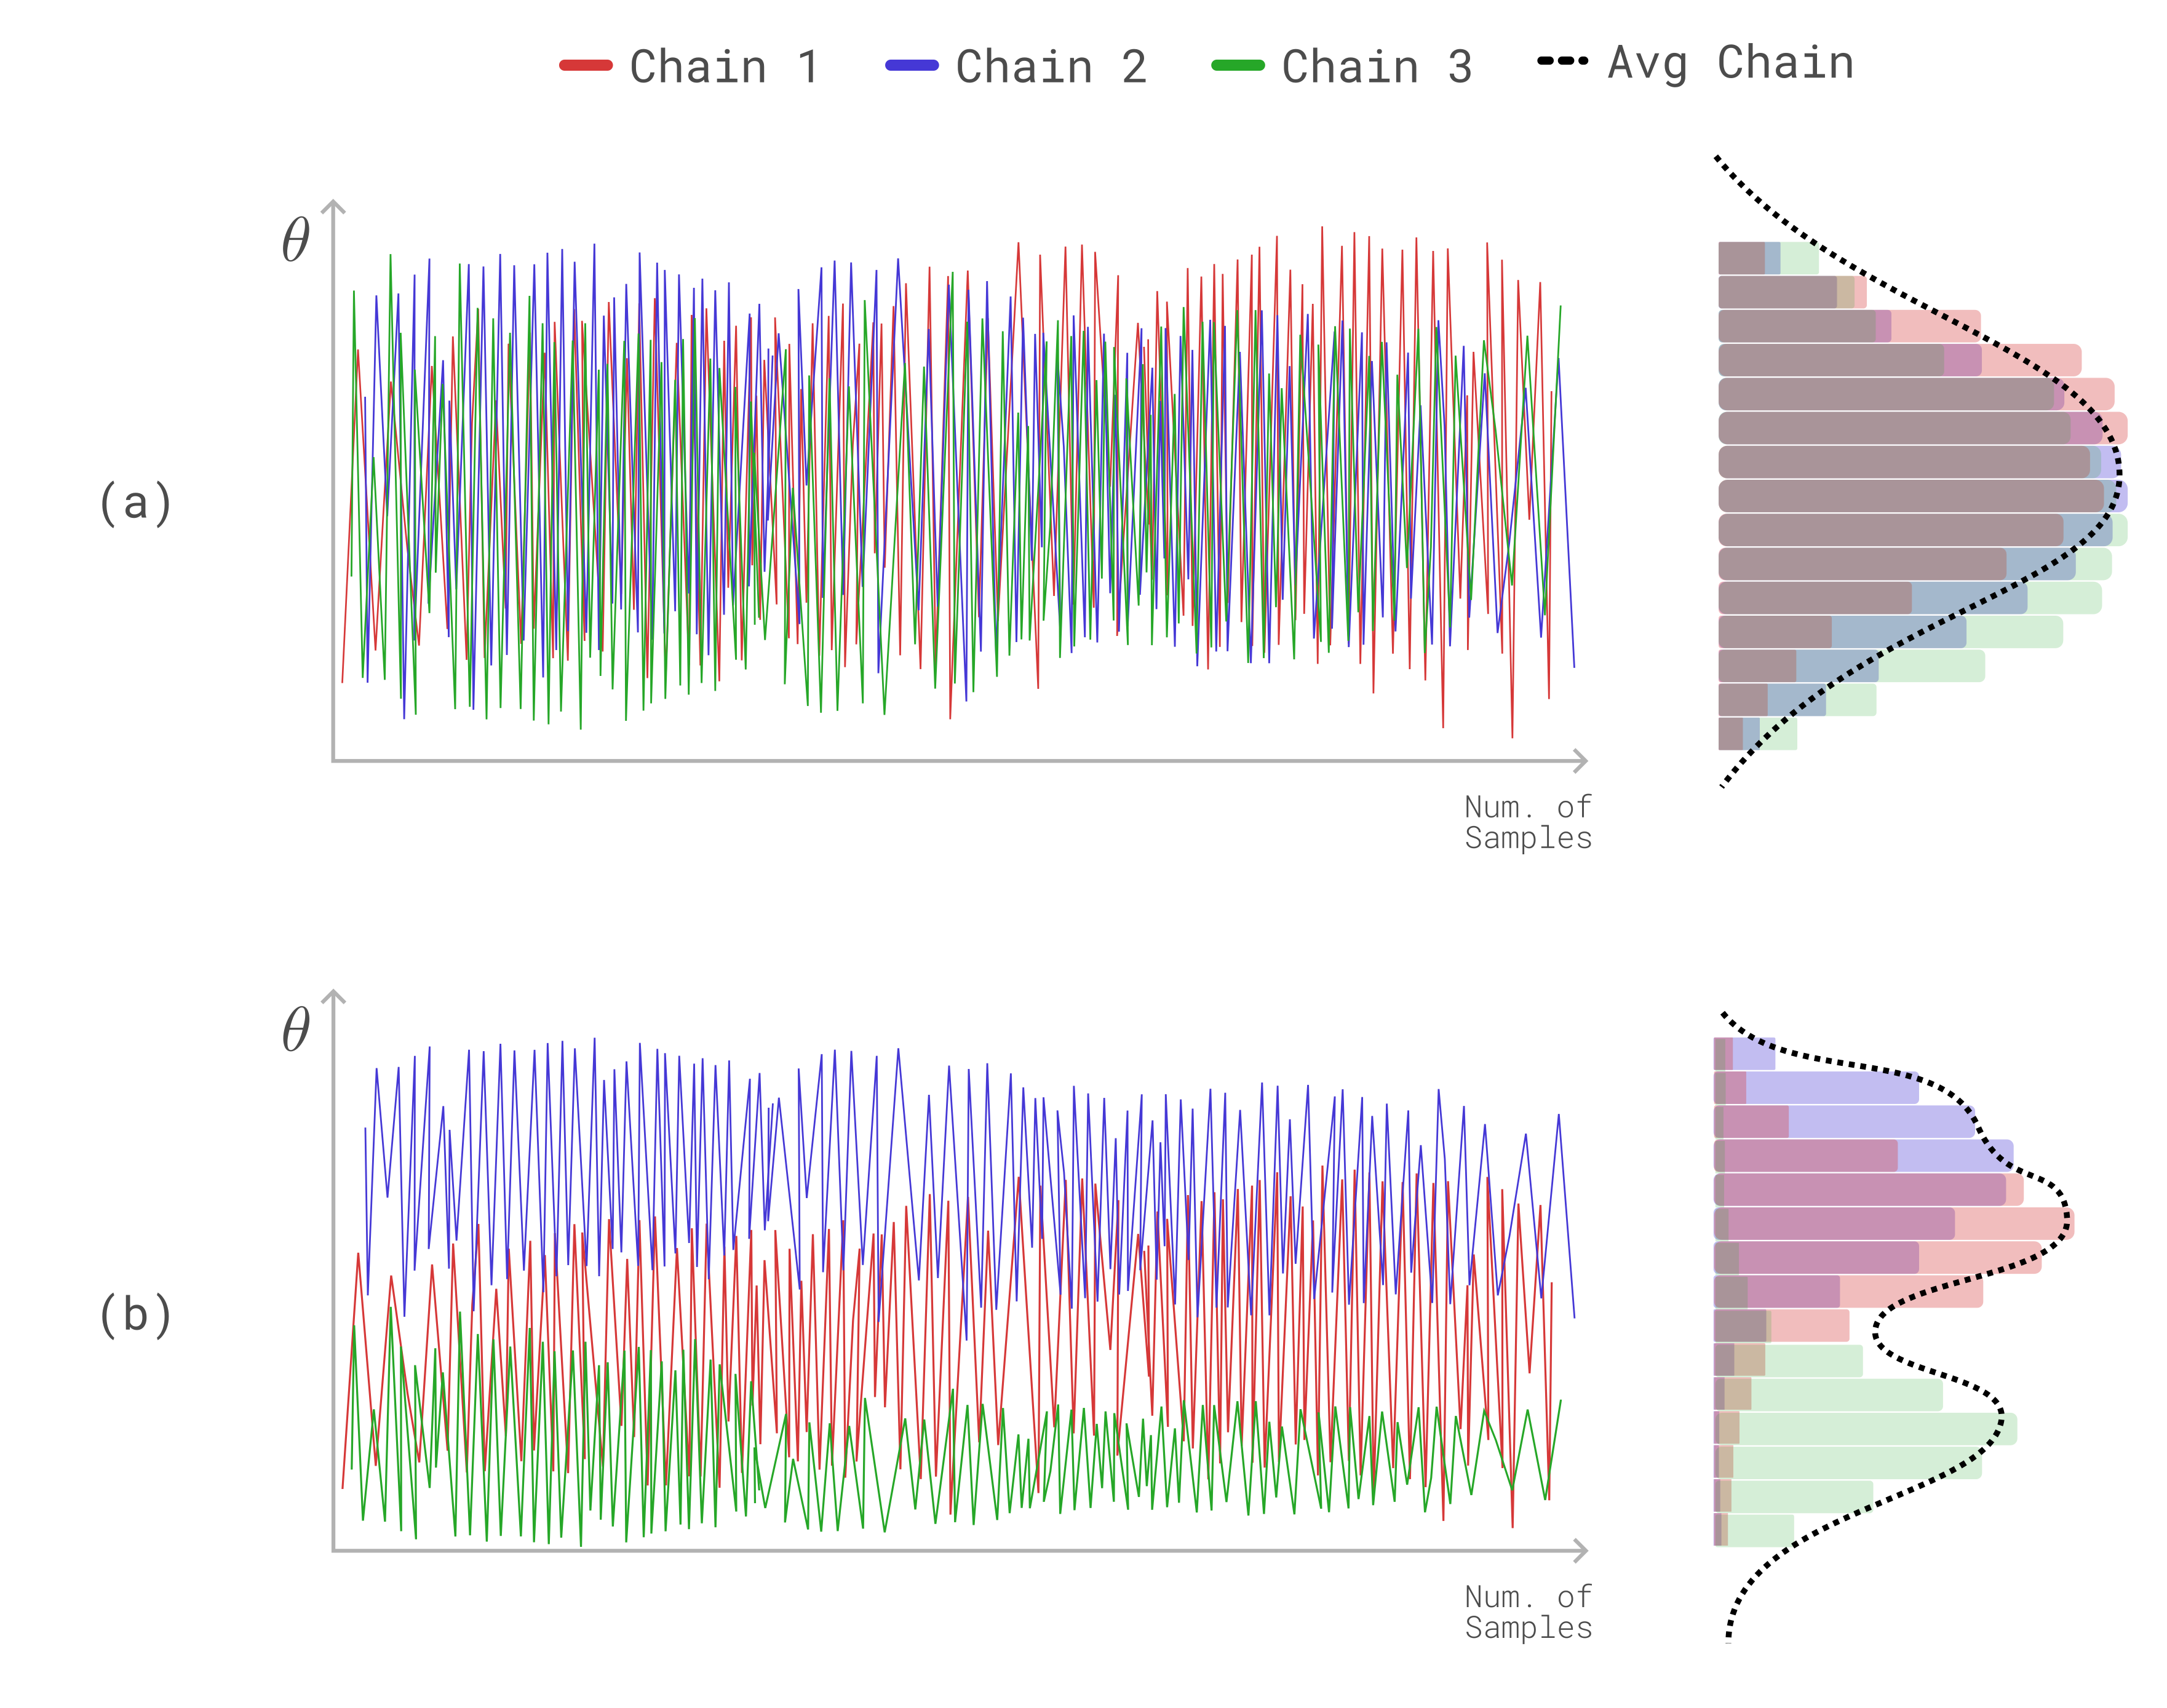
\includegraphics[width=1.0\textwidth]{images/ch3_chain_mix/chain_mix.png}
    \caption{Sampling using multiple chain exploration}
    \label{fig:chains}
\end{figure}

A common practice is to discard several iterations at the beginning of the process. These iterations are known as the warmup of the model and allow the chain to be stable before collecting the samples. Then, the sampling process is repeated multiple times until convergence is guaranteed. Convergence is measured by calculating the within- and between-chain variation, as proposed by \citet{Gelman1992},using the statistic $\hat{R}$ in \Cref{eq:r_hat}.

\begin{equation}\label{eq:r_hat}
    \hat{R} = \sqrt{\frac{W+{\frac{1}{n}}(B-W)}{W}}\\
\end{equation}

\begin{equation}
    W = \frac{1}{m}\sum_{j=1}^{m}s_{j}^{2}\ \ \ \ \ \ \ ; \text{with} \ \ s_{j}^{2}=\frac{1}{n-1}\sum_{i=1}^{n}(\theta_{ij}-\bar{\theta_{j}})^2
\end{equation}

\begin{equation}
    B=\frac{n}{m-1}\sum_{i=1}^{m}(\bar{\theta_{j}}-\bar{\theta})^2
\end{equation}

Where, $W$ is the within-chain variance, $s_j^2$ is the estimator for the sample variance for $j$-th chain, $n$ is the number of samples, $m$ is the number of chains, and $B$ is the between-chain variance. A common rule of convergence is that the statistic $\hat{R}$ should be below 1.01 for each model parameter.

For the analysis performed in this document, a variant of the Hamiltonian Monte Carlo algorithm is used to increase the sampling efficiency. This variant is known as the No U-Turn Sampler (NUTS) and follows the same principles as HMC but dynamically adapts $T$ to increase the sample's acceptance rate.

\subsection{Posterior predictive distribution }

The last section focuses on the use of MCMC methods (HMC in particular) to estimate the posterior distribution of model parameters, which can be used to draw conclusions or perform hypothesis testing. However, the real power of the model is when it is used to predict values in the light of new data. After HMC or any other MCMC algorithm is used to estimate the parameter posterior distributions, these posteriors can be used for prediction. 

The prediction in the Bayesian inference is performed using the following steps, also illustrated in \Cref{fig:posterior_pred}. Although this example corresponds to a univariate linear regression model with one intercept and one slope as model parameters, these steps can be applied in the same way to the multivariate case or any non-linear model: 

\begin{itemize}
    \item Samples from the posterior distribution of the intercept and the slope are collected. 

    \item Each set of parameter samples (intercept-slope) is used to calculate a regression line that produces a new target value. 
    
    \item These target values are known as the \textit{Posterior Predictive distribution}, which is the posterior distribution of the target variable\footnote{Posterior predictive refers to the distribution of the target variable whereas posterior refers to the parameter's distributions.}. 
\end{itemize}

\begin{figure}[H]
    \centering
    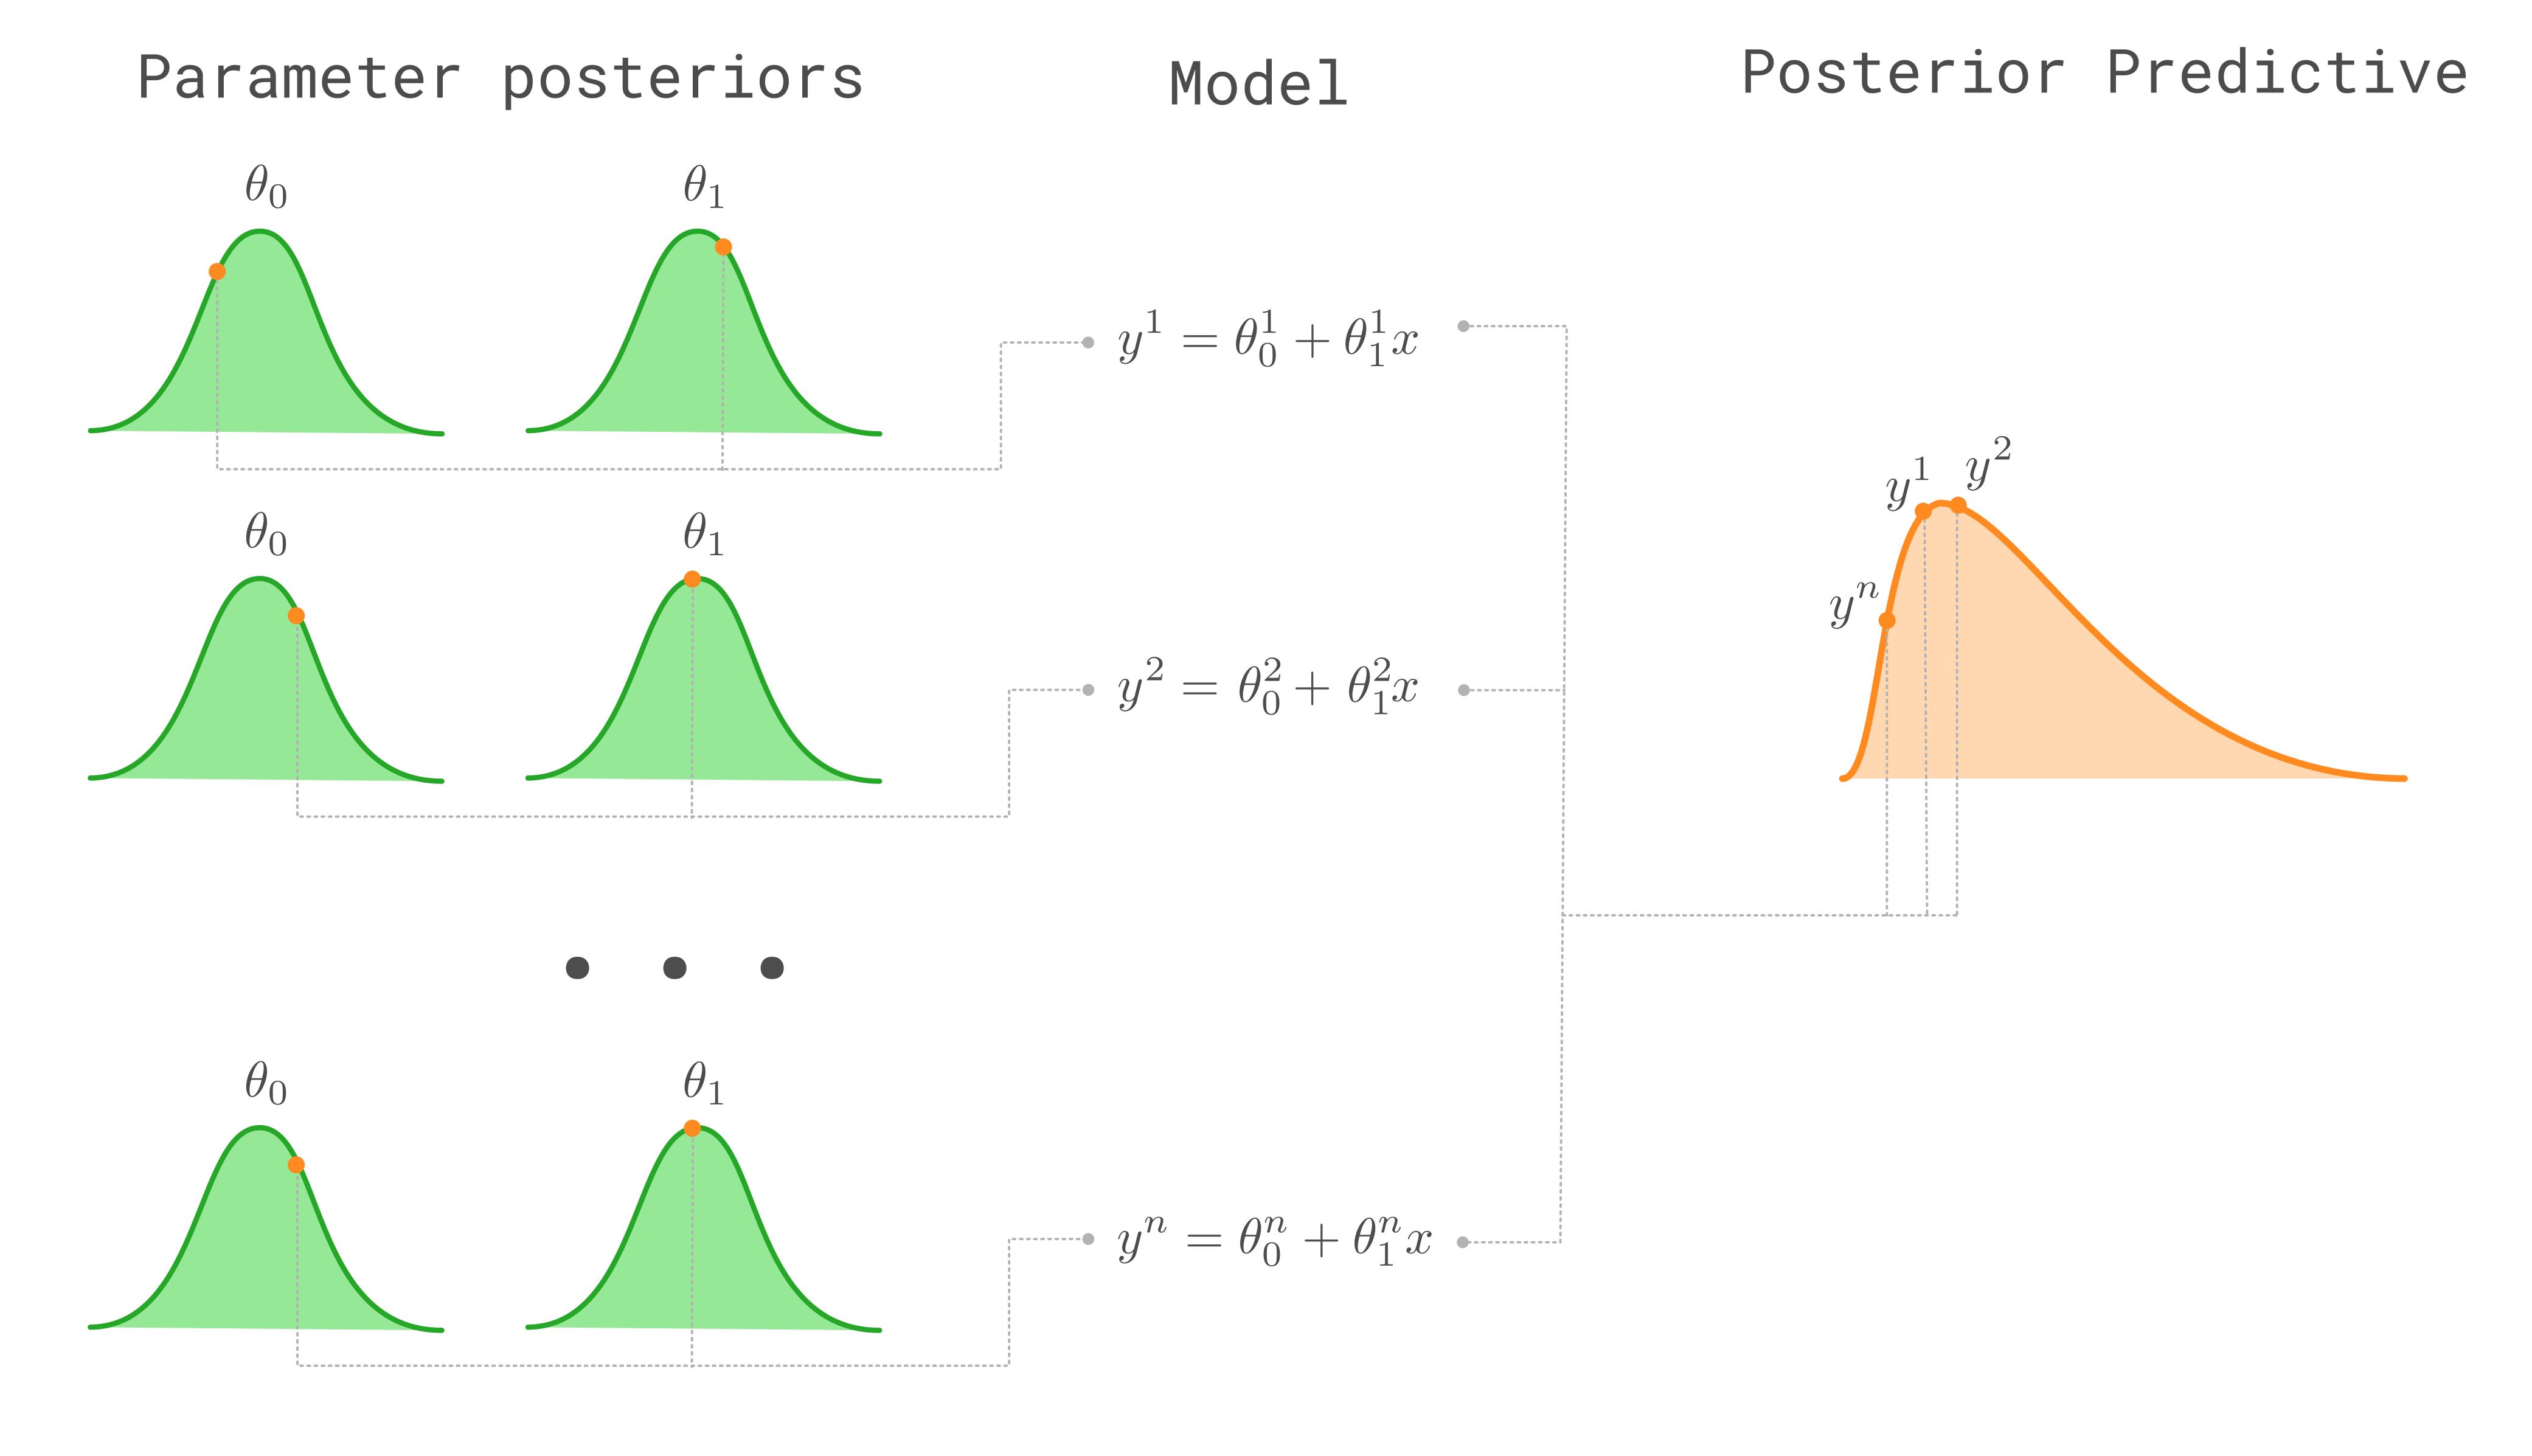
\includegraphics[width=1.0\textwidth]{images/ch3_posterior_pred/posterior_pred.png}
    \caption{Posterior predictive calculation process}
    \label{fig:posterior_pred}
\end{figure}

Once estimated, the posterior predictive distribution is helpful for several use cases: 

\begin{itemize}
    \item In hypothesis testing:
    \begin{itemize}
        \item Compare the posterior distribution within different groups to infer some characteristics from the population of interest. For instance, to measure the gender gap in salaries, the posterior predictive distribution of salaries between men and women can be compared to check the differences and magnitudes. 
    \end{itemize}
    \item For prediction: 
    \begin{itemize}
        \item Calculate point accuracy metrics for the target, such as Mean Squared Error (MSE), Root Mean Squared Error (RMSE), and Mean Absolute Percentage Error (MAPE). 

        \item Evaluate the model accuracy and performance in both in-sample and out-of-sample scenarios by comparing the posterior predictive distribution with the true distribution. 
        
        \item Calculate credible intervals for both the parameters and the target variable to estimate the uncertainty over the target variable through the predictive quantiles (\textit{k-th Percentile of prediction}) 
    \end{itemize}
    \item For simulation:
    \begin{itemize}
        \item Simulate new data that follows the sample distribution of the target variable (in-sample distribution) 

        \item Simulate hypothetical scenarios by changing the parameter's distributions and calculate their effect on the target variable, assuming that the same distribution governs the process. For instance, in the case of testing the impacts of a policy change on the gender gap, assessing the effects on salaries. 
    \end{itemize}
\end{itemize}

\section{Goodness-of-fit and predictive accuracy }\label{section:goodness_of_fit}

Once model parameters are inferred, it is necessary to measure how well the model represents the observed data (in-sample) and its predicting power on new data (out-of-sample). As reviewed in the posterior section, several point estimate metrics, such as MSE, RMSE, and MAE, can measure the model's predicting power. However, as Bayesian predictions are probability distributions, alternative methods that compare the true and the estimated distributions are preferred, as shown in the following subsections. 

\subsection{The ideal measure: Kullback-Leibler Divergence }

Using the theoretical foundations from information theory, the Kullback-Leibler divergence, also known as KL divergence, provides an ideal measure of the discrepancy between two distributions. It measures how much information is lost by using an alternative distribution instead of the true distribution \citep{Lambert2018}. This measure calculates the “distance” between the true distribution $p(x)$ and the alternative distribution $q(x)$, as shown in \Cref{eq:kl_divergence}. In this expression, if the distributions $p(x)$ and $q(x)$ are the same, the $KL$ will be 0. Then, the objective is to build a model that minimizes the $KL$ value.

\begin{align}\label{eq:kl_divergence}
    KL(p \rightarrow q) &= \int_{x \in X} p(x) \log\left(\frac{p(x)}{q(x)}\right) dx \\
    &= \underbrace{\int_{x \in X} p(x) \log(p(x)) dx}_{\text{true distribution}} - \underbrace{\int_{x \in X} p(x) \log(q(x)) dx}_{\text{estimated distribution}}\label{eq:kl_divergence_2} 
\end{align}

The KL divergence can be rewritten as in \Cref{eq:kl_divergence_2}, in which the first term is fixed because it is only related to the true distribution, while the second term is related to the model's choice. Given that the first part is fixed, the KL divergence will be minimized when the second term is maximized. 

In practice, the calculation of the complete KL divergence can be computationally expensive, given the integral calculations. Hence, the second term in the KL divergence can be used as a proxy to reduce the KL divergence using samples from the posterior predictive distribution. This term, also known as \textit{expected log-pointwise predictive density (elppd)}, is the base for comparing the performance between models and calculating some accuracy measures such as the WAIC and LOO-CV.

\subsection{Widely Applicable Information Criterion (WAIC) }

One estimate of the \textit{elppd} can be calculated by summing up the log of the average value of the likelihood across the posterior distribution for each data point $y_i$ used to estimate the model \citep{Gelman2013}, as shown in \Cref{eq:WAIC}. \citet{Gelman2013} recommends applying a \textit{bias} correction term that accounts for the uncertainty in the parameter estimation, and it serves as a regularization term that penalizes the model complexity.

\begin{equation}
    \widehat{elppd} = \sum_{i=1}^{n} \log \left[ E_{\text{posterior}}\left(p(y_i|\theta)\right) \right] - \underbrace{\sum_{i=1}^{n} \text{Var}_{\text{posterior}}\left(\log\left(p(y_i|\theta)\right)\right)}_{\text{bias correction}} \label{eq:WAIC}
\end{equation}

Then, the WAIC score is calculated as $WAIC= -2⋅ \widehat{elppd}$. The lower the WAIC, the better predictive performance of the model18. This score can also be used in model comparison to select the model with the best predictive power. As the WAIC score is calculated with the data points used in the model estimation, it is usually used to measure the model's in-sample predictive power. Nevertheless, if the dataset is split into training, validation, and testing, WAIC calculation using the test set can measure the model's out-of-sample predictive power.

\subsection{LOO-CV} 

Using the basic principle discussed in KL divergence, the method of Leave-one-out cross-validation allows the calculation of the model's out-of-sample predictive power by estimating the model with the $n-1$ data points and calculating the $\widehat{elppd}$ for the remaining datapoint to test the model's performance. The LOO-CV score will be the average of all $\widehat{elppd}$. This approach could be computationally expensive for large datasets, as the model will be re-estimated many times. 

\citet{Vehtari2015} propose an approximation to the LOO-CV score using samples from the posterior distribution estimated with the entire dataset. Therefore, the model will be estimated just once. This method is known as \textit{Pareto Smoothed Importance Sampling (PSIS)}. 

\section{Probabilistic programming: A framework to perform MCMC }

In practice, Bayesian inference is performed using a programming paradigm called Probabilistic programming. This approach combines traditional programming languages with probability theory to handle uncertainty in the modelling process. The general idea in probabilistic programming is that a model corresponds to a series of interconnected random variables, and all calculations are performed using a graph structure. 

There is an ample supply of packages that ease the application of the Bayesian inference framework. Given the author's familiarity with the programming language Python, this thesis uses Numpyro \citep{Phan2019} as the inference library. One interesting characteristic of Numpyro is that it uses JAX for the sampling process. JAX is a powerful library for efficiently performing numerical computation and tensor operations in CPUs, GPUs, TPUs and other multi-device environments. This characteristic is critical given the computational cost of performing Bayesian inference. 
\chapter{Data sources}

\section{Survey of Labour and Income Dynamics - SLID}
\section{Hierarchical structure: Industry and Occupation}
\section{Exploratory Data Analysis}
\chapter{Salary model estimation}

This chapter details the construction of a salary model that predicts annual salaries based on the individual attributes of a worker using the Bayesian inference framework. This model is an update of the current implementation of the wage model in the labour market module of the ILUTE framework presented in \Cref{section:ilute}. 

The content in this chapter is structured into seven subsections: the first part discusses the importance of the hierarchical structure in the model definition. Then, the second section presents the variables used in the model specification. The third section details the model specification based on the findings in the exploratory data analysis in \Cref{section:eda}. The fourth section presents a set of proposed models and the evaluation framework to select the optimal model. The fifth section discusses the model interpretability. The sixth section analyzes the stability of parameters over time, and the final section presents the model validation on data that was not used in the model estimation (out-of-sample). 

\section{Data structure: from single to multilevel structure}

The previous sections discussed how a linear combination of some personal attributes can explain salaries. Additionally, it explored how salary variability is attributable to the hierarchical structure defined by the industry and occupation categories. Therefore, exploring the data structure and data generation process before modelling salaries is important for defining the best approach. 

Considering these factors, a simple linear combination of personal characteristics, also known as a \textit{\textbf{Pooled model}}, can be one way to model salaries. In this approach, all industries and occupations are equally treated, which implies that salaries are modelled as the average for all industries and occupations. Although theoretically correct, this model type fails to represent the structure of the industry-occupation relationship and produces poor goodness-of-fit and low performance in the long run. One example of this approach is a linear regression that predicts salaries using the data from the whole labour market. This model will predict the average salary but certainly will overestimate the value for low-skill jobs and underestimate salaries for high-skill jobs. 

 One way to improve the pooled model performance is to estimate one linear model for each hierarchy level. That means estimating one linear regression for each industry-occupation combination in the labour market. This approach, also known as the \textit{\textbf{No-Pooled model}}, captures the hierarchical structure with the downside that it treats each industry-occupation combination as totally independent from the other ones. This independence assumes that salaries in the same industry but in different occupations are unrelated, contrary to the nested characteristic observed in the exploratory data analysis section. 

This independence results in a model that is less robust to outliers, prone to overfit the data, and hard to meet the statistical significance for industry-occupation categories with a small number of data points. Ultimately, these disadvantages affect the model's performance and the goodness-of-fit in the no-pooled approach. Therefore, an implementation that accounts for the hierarchy in the data and the internal relationships is needed to predict and model salaries adequately.  

Taking the no-pooled approach as a base, this model can be improved by introducing some dependency between industry-occupation classes. The \textit{\textbf{Multilevel or Hierarchical model}} is an approach between the last two model types. It represents each industry-occupation combination as a separate model but draws information from higher levels (industry level) to produce more realistic predictions. By using information from higher levels, the model is more robust to outliers, less prone to overfit, and produces more realistic predictions because it considers the inner relationships. 

One interesting way to understand the advantages of using the hierarchical model over the other approaches is through the \textit{Simpson's paradox}. Using the synthetic salary and experience dataset shown in \Cref{fig:simpsons_paradox} with some artificial categories (one industry and three occupations within that industry), the pooled model (grey line) predicts that salaries decrease with experience. In contrast, the no-pooled model (dashed lines) captures the expected behaviour in which salary increases with experience. The Hierarchical model (solid lines) provides the most reliable estimation in this conceptual demonstration because it captures the expected behaviour and is less sensitive to outliers. This performance improvement comes with an increase in computational costs. 

\begin{figure}[H]
    \centering
    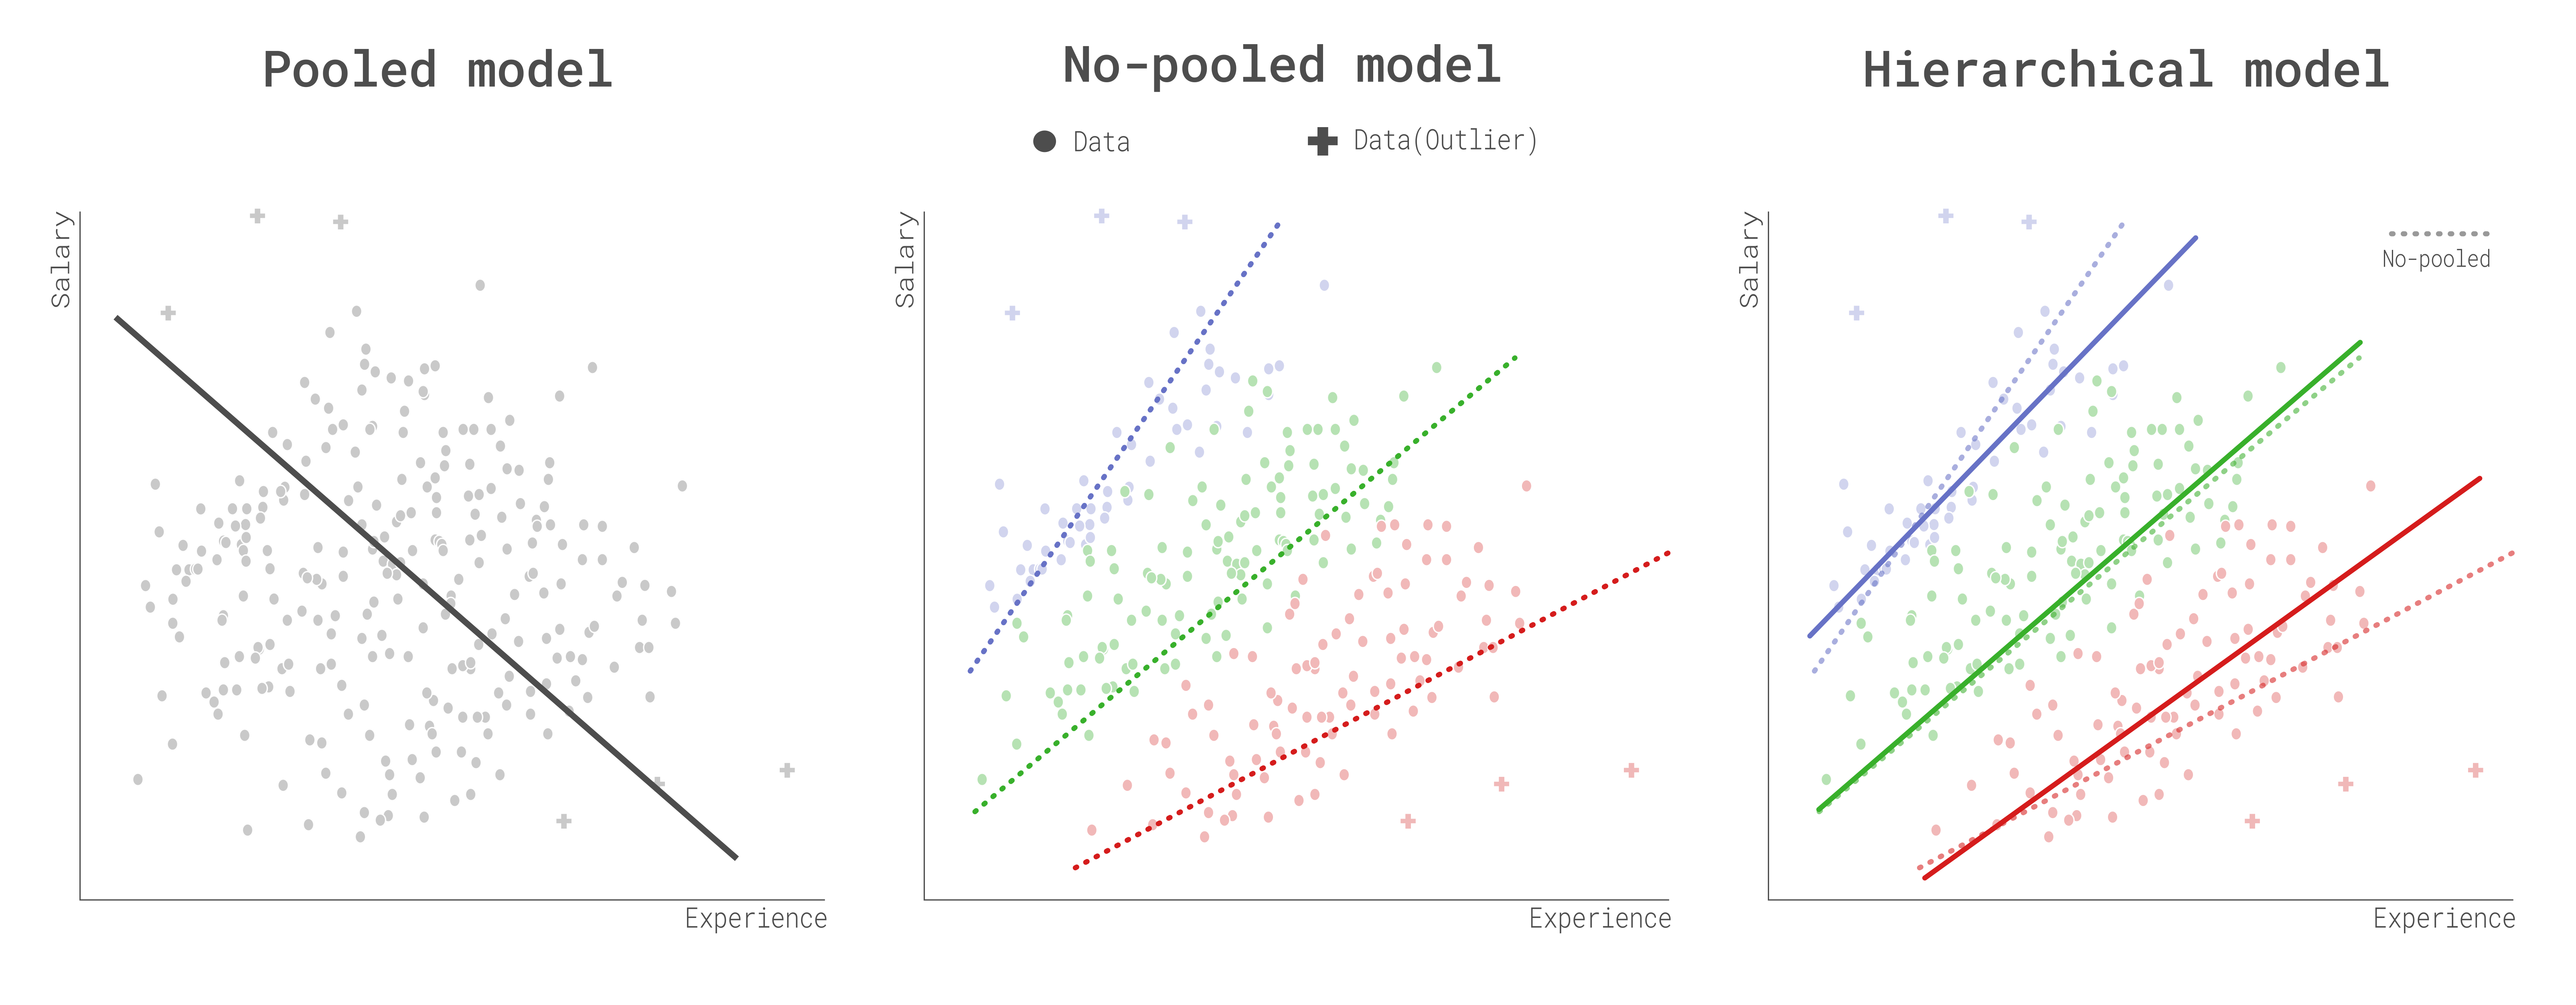
\includegraphics[width=1.0\textwidth]{images/ch5_simpsons_paradox/simpsons_paradox.png}
    \caption{Effect of model structure on the data representation}
    \label{fig:simpsons_paradox}
\end{figure}

Given that the hierarchical approach draws information from the higher level (industry level), salaries predicted for each category tend to move towards the average industry value, represented by the dashed lines in \Cref{fig:simpsons_paradox}. This behaviour is known as \textit{Shrinkage}, which can be interpreted as a regularization process that increases the model's robustness by reducing the effect of outliers and the risk of overfitting. 

As a brief overview, the following list and \Cref{fig:model_structure} summarize the differences in the inference process for the three approaches\footnote{There are similar model structures in the frequentist approach. The pooled and no-pooled counterpart could be a set of simple linear regressions or ANOVA models, and the Hierarchical model is known in the frequentist framework as a mixed-effects model. Numerous examples also exist in the random utility / discrete choice modelling literature.}

\begin{itemize}
    \item \textbf{Pooled model}: In this approach, the modeller defines a set of priors for each model parameter based on the existing knowledge. Then, the posterior distribution for each model parameter is estimated using the Bayesian framework reviewed in \Cref{chapter:bayesian_inference}. The posterior distributions represent the average value of each parameter for all industries and occupations. 

    \item \textbf{No-pooled model}: In this approach, each industry-occupation combination has a set of priors for each model parameter. Each prior is defined by the modeller based on the existent knowledge. Then, the estimation result is a distribution matrix for each model parameter. Each distribution in this matrix corresponds to the estimated posterior distribution for that specific industry occupation and that given parameter. 
    
    \item \textbf{Multilevel or Hierarchical model}: This approach follows the same process as the No-pooled model, adding an extra step before setting the priors. One of the key characteristics of the hierarchical models is the transfer of information between higher and lower levels. This is achieved by setting a set of hyperpriors that defines the localization and scale of the prior distributions (prior parameters). In the hierarchical approach, the modeller only defines the shape of the prior distribution and lets the data select the best parameters for that prior based on the hyperpriors. After the estimation process, a matrix of distributions for each model parameter is generated. Each one of these distributions corresponds to the estimated posterior distribution for that specific industry occupation and for that given parameter. However, each distribution shares information with other distributors in the same industry. The estimation process also provides posterior distributions for the hyperpriors, which corresponds to the distribution of the information shared across categories in the same industry. This process makes the hierarchical approach robust and powerful for modelling complex data structures.
\end{itemize}

\begin{figure}[H]
    \centering
    \includegraphics[width=0.78\textwidth]{images/ch5_model_structure/model_structure.png}
    \setlength{\abovecaptionskip}{-12pt}
    \caption{Inference process by model structure}
    \label{fig:model_structure}
\end{figure}

Despite these approaches exemplified in this section using linear models, it is important to highlight that these structures are model agnostic, which means that they can be used with linear and non-linear models. Therefore, the three approaches reviewed in this section only define the model structure. 

Based on these arguments, the Hierarchical structure seems to be the best option for modelling salaries using the SLID dataset. However, the model specification and selection sections compare the three approaches to measure their performance using the SLID data. In the model selection, the optimal model is chosen based on the measures reviewed in \Cref{section:goodness_of_fit}.

\section{Model variables}

The variables used in the model estimation are detailed in \Cref{table:model_vars}. It is important to highlight that all variables are used to select the model structure. After choosing the optimal structure, the final variables are selected through a Forward selection process, as presented in \Cref{section:model_selection}.

Based on the comments of \citet{Harmon2013}, the underestimation of the existent wage model could be related to the quality of the hourly salary data. Therefore, the proposed model uses annual salary as the target variable instead of the hourly wage. 

The original SLID dataset is split into two: from 1996 to 2007 and 2008 to 2011. The first corresponds to the dataset used in the model estimation, and the last is the dataset used in the validation section. 

\renewcommand{\arraystretch}{1.5}
\begin{table}[H]
    \begin{tabular}{p{2cm}p{4cm}p{2cm}p{7cm}}
        \textbf{Name} & \textbf{Units} & \textbf{Type} & \textbf{Description} \\
        \hline
        \rowcolor{lightgray} Experience & years & Continuous & Years of previous experience in the occupation and industry \\

        Sex & 0 or 1 & Categorical & Dummy variable that takes 0 for Males or 1 for Females \\

        \rowcolor{lightgray} Education Level & 0 or 1 for each education level: \newline No education, \newline Elementary, \newline High-school, \newline Postsecondary, \newline Undergraduate, \newline Graduate & Categorical & The dummy variable represents the education level using a One-hot encoding. \\

        Age & years (15-99) & Continuous & Age of the individual at the time of the survey \\

        \rowcolor{lightgray} Tenure & months & Continuous & Number of months in the same job \\

        Union & 0 or 1 & Categorical & Dummy variable that takes 1 if the individual is unionized or 0 otherwise \\

        \rowcolor{lightgray} Public sector & 0 or 1 & Categorical & The dummy variable takes 1 if the individual works in the public sector and 0 otherwise. \\

        Self-employment & 0 or 1 & Categorical & The dummy variable takes 1 if the individual is self-employed and 0 otherwise. \\

        \hline
    \end{tabular}
    \caption{\label{table:model_vars} Variables used in the model specification}
\end{table}


\section{Model specification}

Once the model structure and data variables are defined, it is necessary to specify the relationships between the variables of interest in the model by recreating the data generation process. Two of the most relevant characteristics of the data generation process are the distribution of the target variable and the relationships between the explanatory variables. 

As discussed in the exploratory data analysis section, salaries are positive and right-skewed distributed, which resembles the Gamma distribution. On the other hand, theoretical models explored in the literature review section show how the salary of a particular worker can be explained by using a linear combination of different personal attributes such as education level, experience, gender, and age, among others. Hence, the model specification must meet these target distribution and linearity requirements. 

A model that meets these requirements is the \textit{Gamma Generalized Linear Model (Gamma GLM)}, which belongs to the family of linear models that represents a process in terms of a linear combination with error distribution different from the normal distribution, as in the ordinary linear regression \citep{Nielsen2010}.

Given a set of explanatory variables $X=[X_1,X_2,...,X_p]$ and a set of model parameters $\theta = [\theta_0,\theta_1,...,\theta_p]$, the Gamma GLM is defined by the following components:

\begin{itemize}
    \item \textbf{Random component}: The response variable $Y$ follows a Gamma distribution (\Cref{eq:gamma_distribution}) defined by the parameters $\alpha$ and $\beta$ (shape and scale respectively). The expected value of this distribution is $\mu=\frac{\alpha}{\beta}$
    \begin{equation}\label{eq:gamma_distribution}
        f(y,\alpha, \beta)=\frac{\beta^\alpha}{\varGamma(\alpha)}y^{\alpha-1}e^{-\beta y} \text{ \\ \\ \\  , \\  \\ } y > 0
    \end{equation}
    \item \textbf{Systematic component}: The linear combination $\eta$ of explanatory variables $X$ and the model parameters $\theta$.
    \begin{equation}
        \eta = \theta_0 + \theta_1X_1+\theta_2X_2+...+\theta_pX_p
    \end{equation}
    \item \textbf{Link function}: This function connects the expected value of the target variable with the linear predictor $\eta$ using a log link and ensures that the linear predictor is positive and continuous. When solved for $\mu$, it provides the expectation over the target variable.
    \begin{align}
        \begin{split}
            log(\mu) &= \eta\\
            \mu &= e^{\eta}=e^{\theta_0+\theta_1X_1+...+\theta_pX_p}
        \end{split}
    \end{align}
\end{itemize}

Hence, the inference process is focused on estimating the parameters $\theta$'s in the systematic component, whereas the parameters $\alpha$ and $\beta$ in the random component are inferred indirectly using the systematic component and the log-link function. The following subsections present the model specification of the Gamma GLM for each model structure (Pooled, No-Pooled, and Hierarchical). 

\subsection{Pooled model}

\Cref{eq:pooled_model} presents the model specification for the Pooled structure and \Cref{fig:model_graph_pooled}. Model graph - Pooled shows the model graph. The expression \Cref{eq:pooled_model}-[1] corresponds to the random component, while the expressions \Cref{eq:pooled_model}-[2] and \Cref{eq:pooled_model}-[4] correspond to the priors for the model parameters $\theta_p$ and $\alpha$. The model parameters correspond to all variables listed in \Cref{table:model_vars}.

\begin{gather}
    \begin{split}
        Y \sim Gamma(\alpha,\beta) \quad \textcolor{gray}{[\text{1}]} \\
        \alpha \sim Uniform(0, 100) \quad \textcolor{gray}{[\text{2}]} \\
        \beta=\alpha/\mu \quad \textcolor{gray}{[\text{3}]} \\
        \theta_{p} \sim Normal(0, 1) \quad \textcolor{gray}{[\text{4}]} \\
        \mu=e^{\theta_0+\theta_{1}X_{1}+...+\theta_{p}X_{p}} \quad \textcolor{gray}{[\text{5}]} \\
    \end{split}
    \label{eq:pooled_model}
\end{gather}

The choice of the priors is given by: 
\begin{itemize}
    \item For the parameters $\theta$'s, the prior selected is the normal distribution with mean 0 and sigma 1. The mean centred in 0 ensures that the parameters can take positive or negative values according to the relationships in the data. 

    \item For the parameter $\alpha$, the prior selected is the uniform distribution with lower limit 0 and upper limit 100. The uniform distribution is a non-informative prior that ensures different values for $\alpha$ are tested with equal probability of occurrence. This choice is made because there is no evidence of the $\alpha$ value in previous salary prediction exercises. 
    
    \item The parameter $\beta$ does not require a prior because it is calculated based on the other parameters. 
\end{itemize}

\begin{figure}[H]
    \centering
    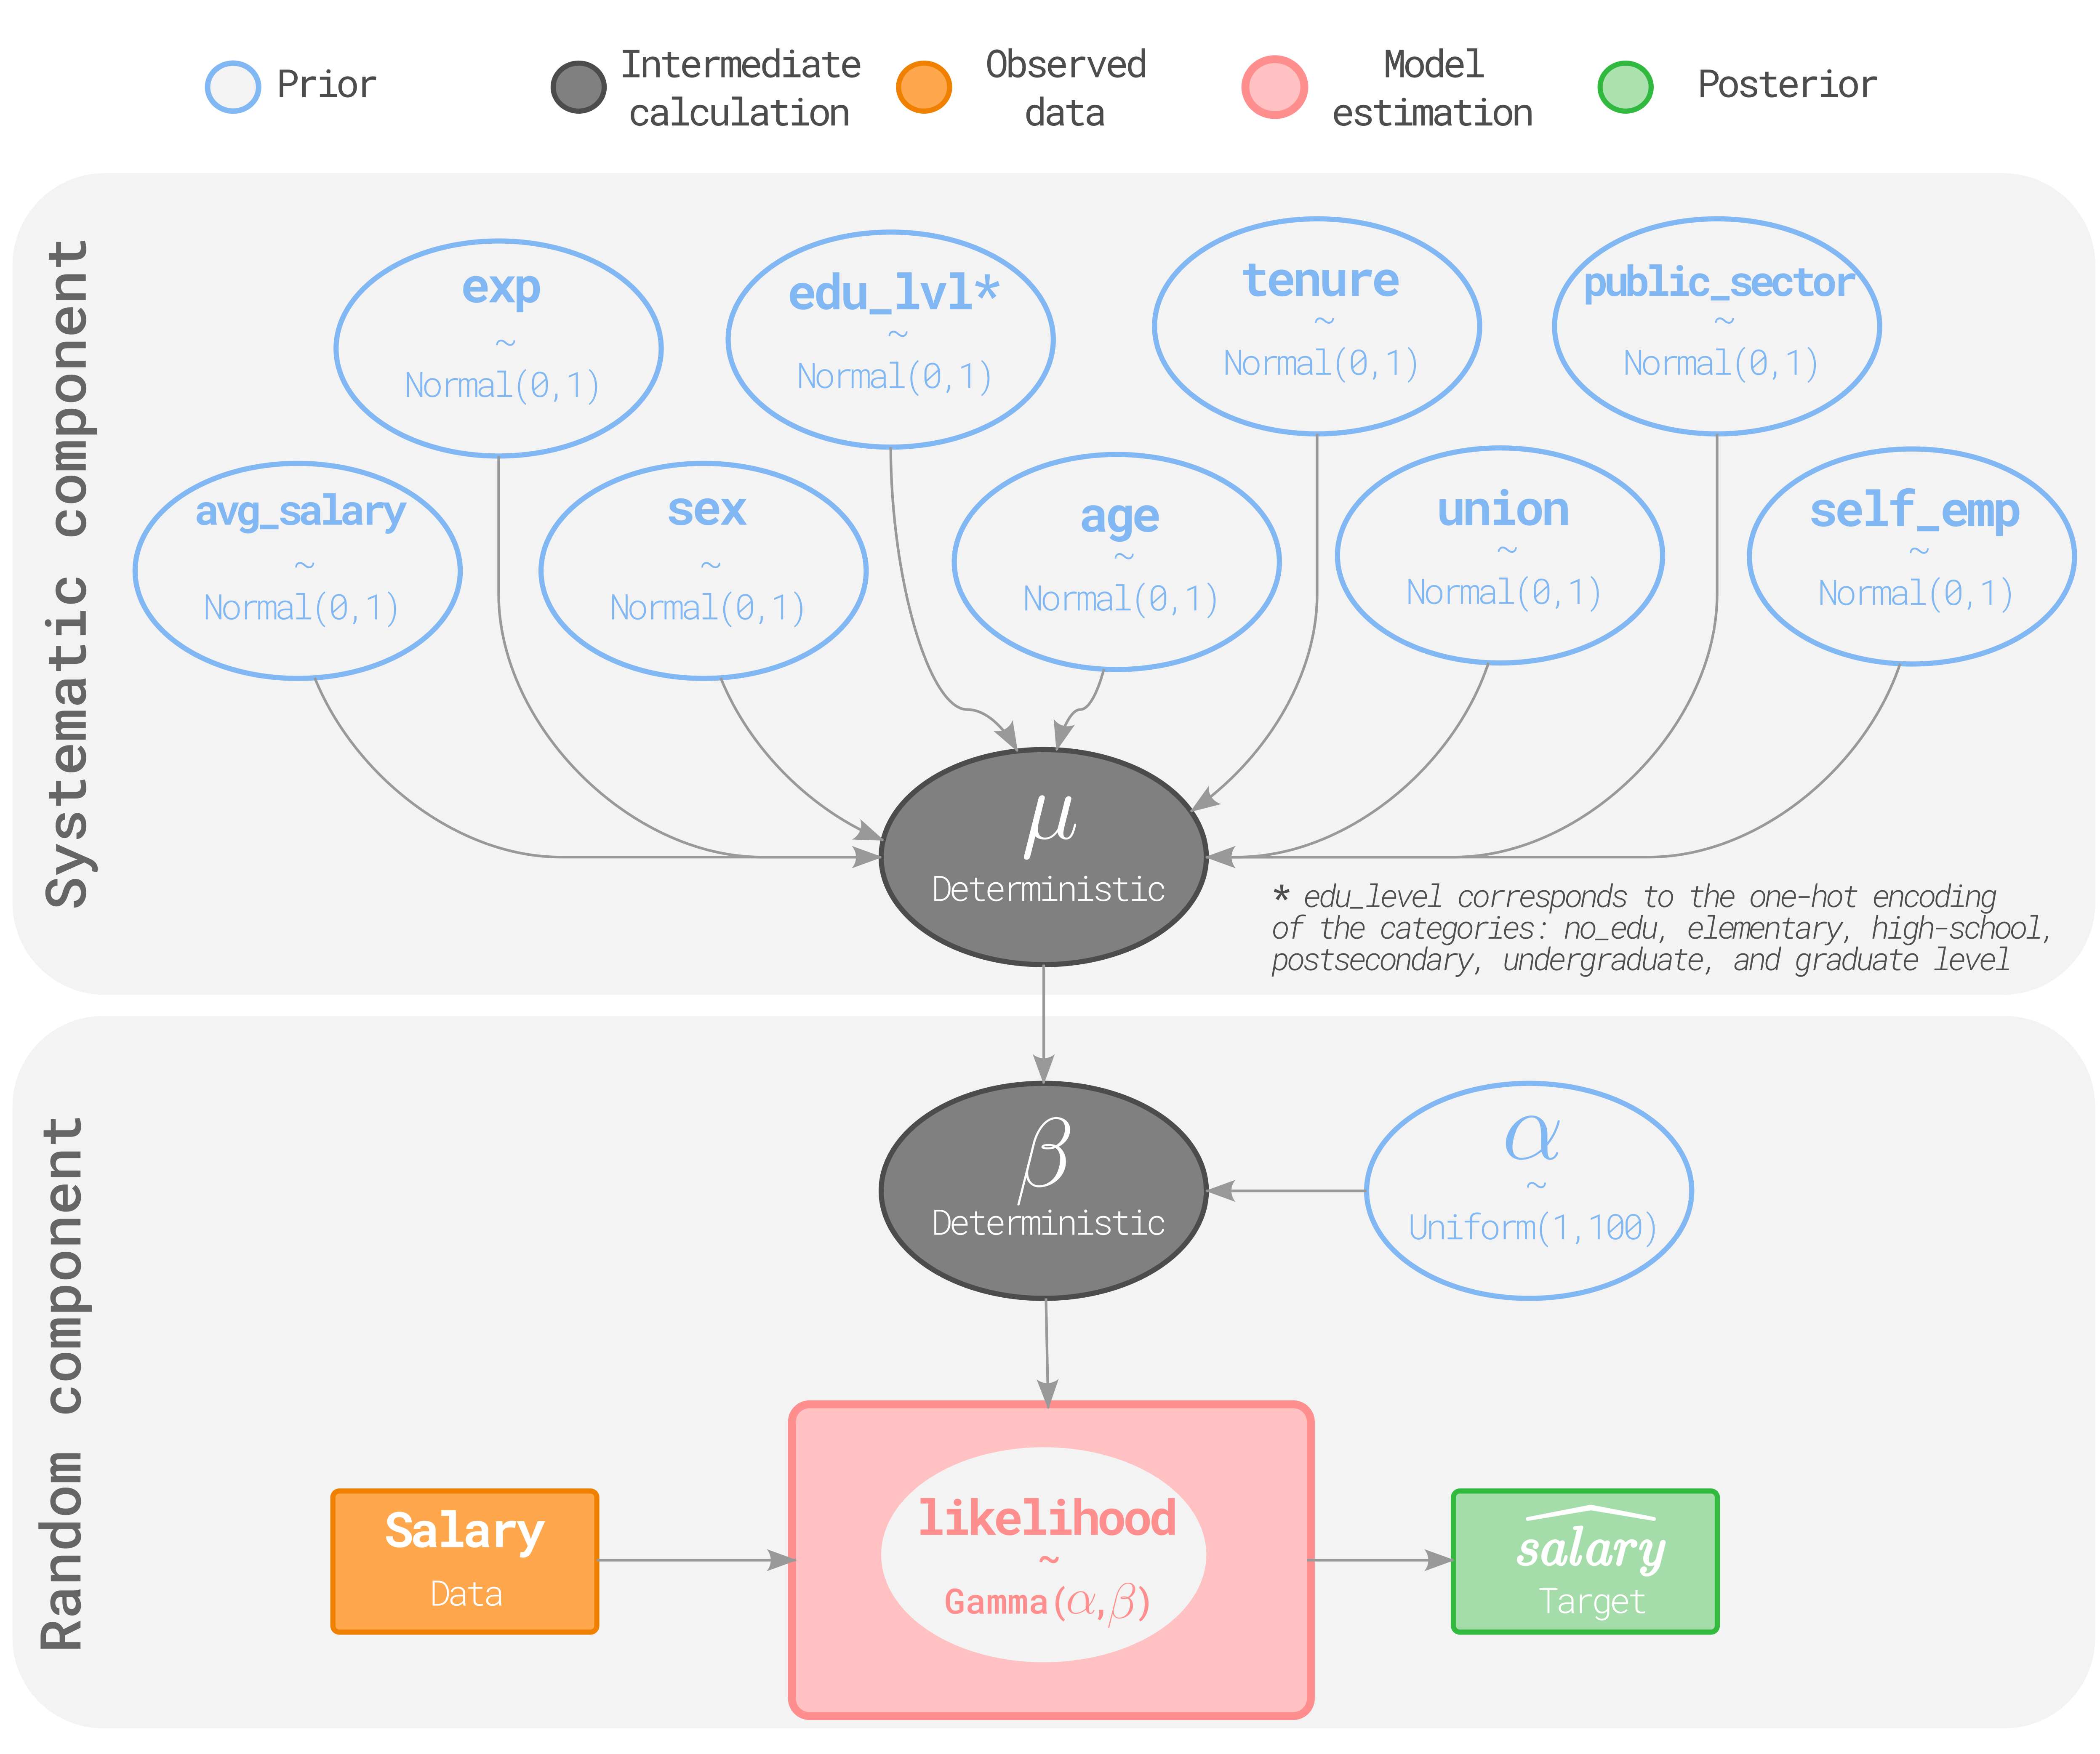
\includegraphics[width=0.96\textwidth]{images/ch5_pooled_graph/pooled_graph.png}
    \setlength{\abovecaptionskip}{-12pt}
    \caption{Model graph - Pooled}
    \label{fig:model_graph_pooled}
\end{figure}

\subsection{No-pooled model} 

\Cref{eq:no_pooled_model} presents the model specification for the No-pooled structure, and \Cref{fig:model_graph_nopooled} shows the model graph. The model parameters correspond to all variables listed in \Cref{table:model_vars}. The superscripts $ind$  and $occ$ correspond to each hierarchy level (industries and occupations) presented in \Cref{section:hierarchy}. 

\begin{gather}
    \begin{split}
        Y \sim Gamma(\alpha,\beta) \quad \textcolor{gray}{[\text{1}]} \\
        \alpha \sim Uniform(0, 100) \quad \textcolor{gray}{[\text{2}]} \\
        \beta=\alpha/\mu \quad \textcolor{gray}{[\text{3}]} \\
        \theta_{p}^{ind} \sim Normal(0, 1) \quad \textcolor{gray}{[\text{4}]} \\
        \theta_{p}^{occ} \sim Normal(0, 1) \quad \textcolor{gray}{[\text{5}]} \\
        \eta^{ind} = \theta_0^{ind}+\theta_1^{ind}X_1+...+\theta_p^{ind}X_p \quad \textcolor{gray}{[\text{6}]} \\
        \eta^{occ} = \theta_0^{occ}+\theta_1^{occ}X_1+...+\theta_p^{occ}X_p \quad \textcolor{gray}{[\text{7}]} \\
        \mu=e^{\eta^{ind}+\eta^{occ}} \quad \textcolor{gray}{[\text{8}]} \\
    \end{split}\label{eq:no_pooled_model}
\end{gather}

Like in the Pooled model, the choice of the priors in the No-pooled model is given by: 
\begin{itemize}
    \item For the parameters $\theta$'s for both $ind$ and $occ$, the prior selected is the normal distribution with mean 0 and sigma 1. 

    \item For the parameter $\alpha$, the prior selected is the uniform distribution with lower limit 0 and upper limit 100. 
    
    \item The parameter $\beta$ does not require a prior because it is calculated based on the other parameters. 
\end{itemize}

\begin{figure}[H]
    \centering
    \includegraphics[width=0.96\textwidth]{images/ch5_no_pooled_graph/no_pooled_graph.png}
    \setlength{\abovecaptionskip}{-12pt}
    \caption{Model graph - No-pooled}
    \label{fig:model_graph_nopooled}
\end{figure}

\subsection{Hierarchical model}

\Cref{eq:hierarchical_model} presents the model specification for the Hierarchical model, and \Cref{fig:model_graph_hierarchical} shows the model graph. The hierarchical model uses the variables listed in \Cref{table:model_vars} and superscripts $ind$  and $occ$ presented in \Cref{section:hierarchy}. However, it adds two hyperpriors (one for the localization parameter and one for the scale parameter) that share information from a higher to a lower level. These hyperpriors are defined for both the industry and occupation level.  

 \begin{gather}
    \begin{split}
        Y \sim Gamma(\alpha,\beta) \quad \textcolor{gray}{[\text{1}]} \\
        \alpha \sim Uniform(0, 100) \quad \textcolor{gray}{[\text{2}]} \\
        \beta=\alpha/\mu \quad \textcolor{gray}{[\text{3}]} \\
        loc_{p}^{ind} \sim Normal(0,1) \quad \textcolor{gray}{[\text{4}]} \\
        scale_{p}^{ind} \sim HalfNormal(1) \quad \textcolor{gray}{[\text{5}]} \\
        loc_{p}^{occ} \sim Normal(0,1) \quad \textcolor{gray}{[\text{6}]} \\
        scale_{p}^{occ} \sim HalfNormal(1) \quad \textcolor{gray}{[\text{7}]} \\
        \theta_{p}^{ind} \sim Normal(loc_{p}^{ind}, scale_{p}^{ind}) \quad \textcolor{gray}{[\text{8}]} \\
        \theta_{p}^{occ} \sim Normal(loc_{p}^{occ}, scale_{p}^{occ}) \quad \textcolor{gray}{[\text{9}]} \\
        \eta^{ind} = \theta_0^{ind}+\theta_1^{ind}X_1+...+\theta_p^{ind}X_p \quad \textcolor{gray}{[\text{10}]} \\
        \eta^{occ} = \theta_0^{occ}+\theta_1^{occ}X_1+...+\theta_p^{occ}X_p \quad \textcolor{gray}{[\text{11}]} \\
        \mu=e^{\eta^{ind}+\eta^{occ}} \quad \textcolor{gray}{[\text{12}]} \\
    \end{split}\label{eq:hierarchical_model}
 \end{gather}

 The choice of the priors in the Hierarchical model is given by: 
\begin{itemize}
    \item For the hyperprior $loc_p^*$, the distribution selected is the Normal distribution with mean 0 and sigma 1. That allows the model to choose the best value according to the observed data and share the same distribution for occupations in the same industry. 

    \item Likewise, the hyperprior $scale_p^*$ is defined with the Half-Normal distribution with sigma 1. This distribution ensures that all values are positive, which is mandatory given that $scale_p^*$ is the sigma value in the correspondent prior $\theta_p^*$. 

    \item For the parameters $\theta$'s for both $ind$ and $occ$, the prior selected is the normal distribution with mean $loc_p^*$ and sigma $scale_p^*$. 

    \item For the parameter $\alpha$, the prior selected is the uniform distribution with lower limit 0 and upper limit 100. 

    \item The parameter $\beta$ does not require a prior because it is calculated value. 
\end{itemize}

\begin{figure}[H]
    \centering
    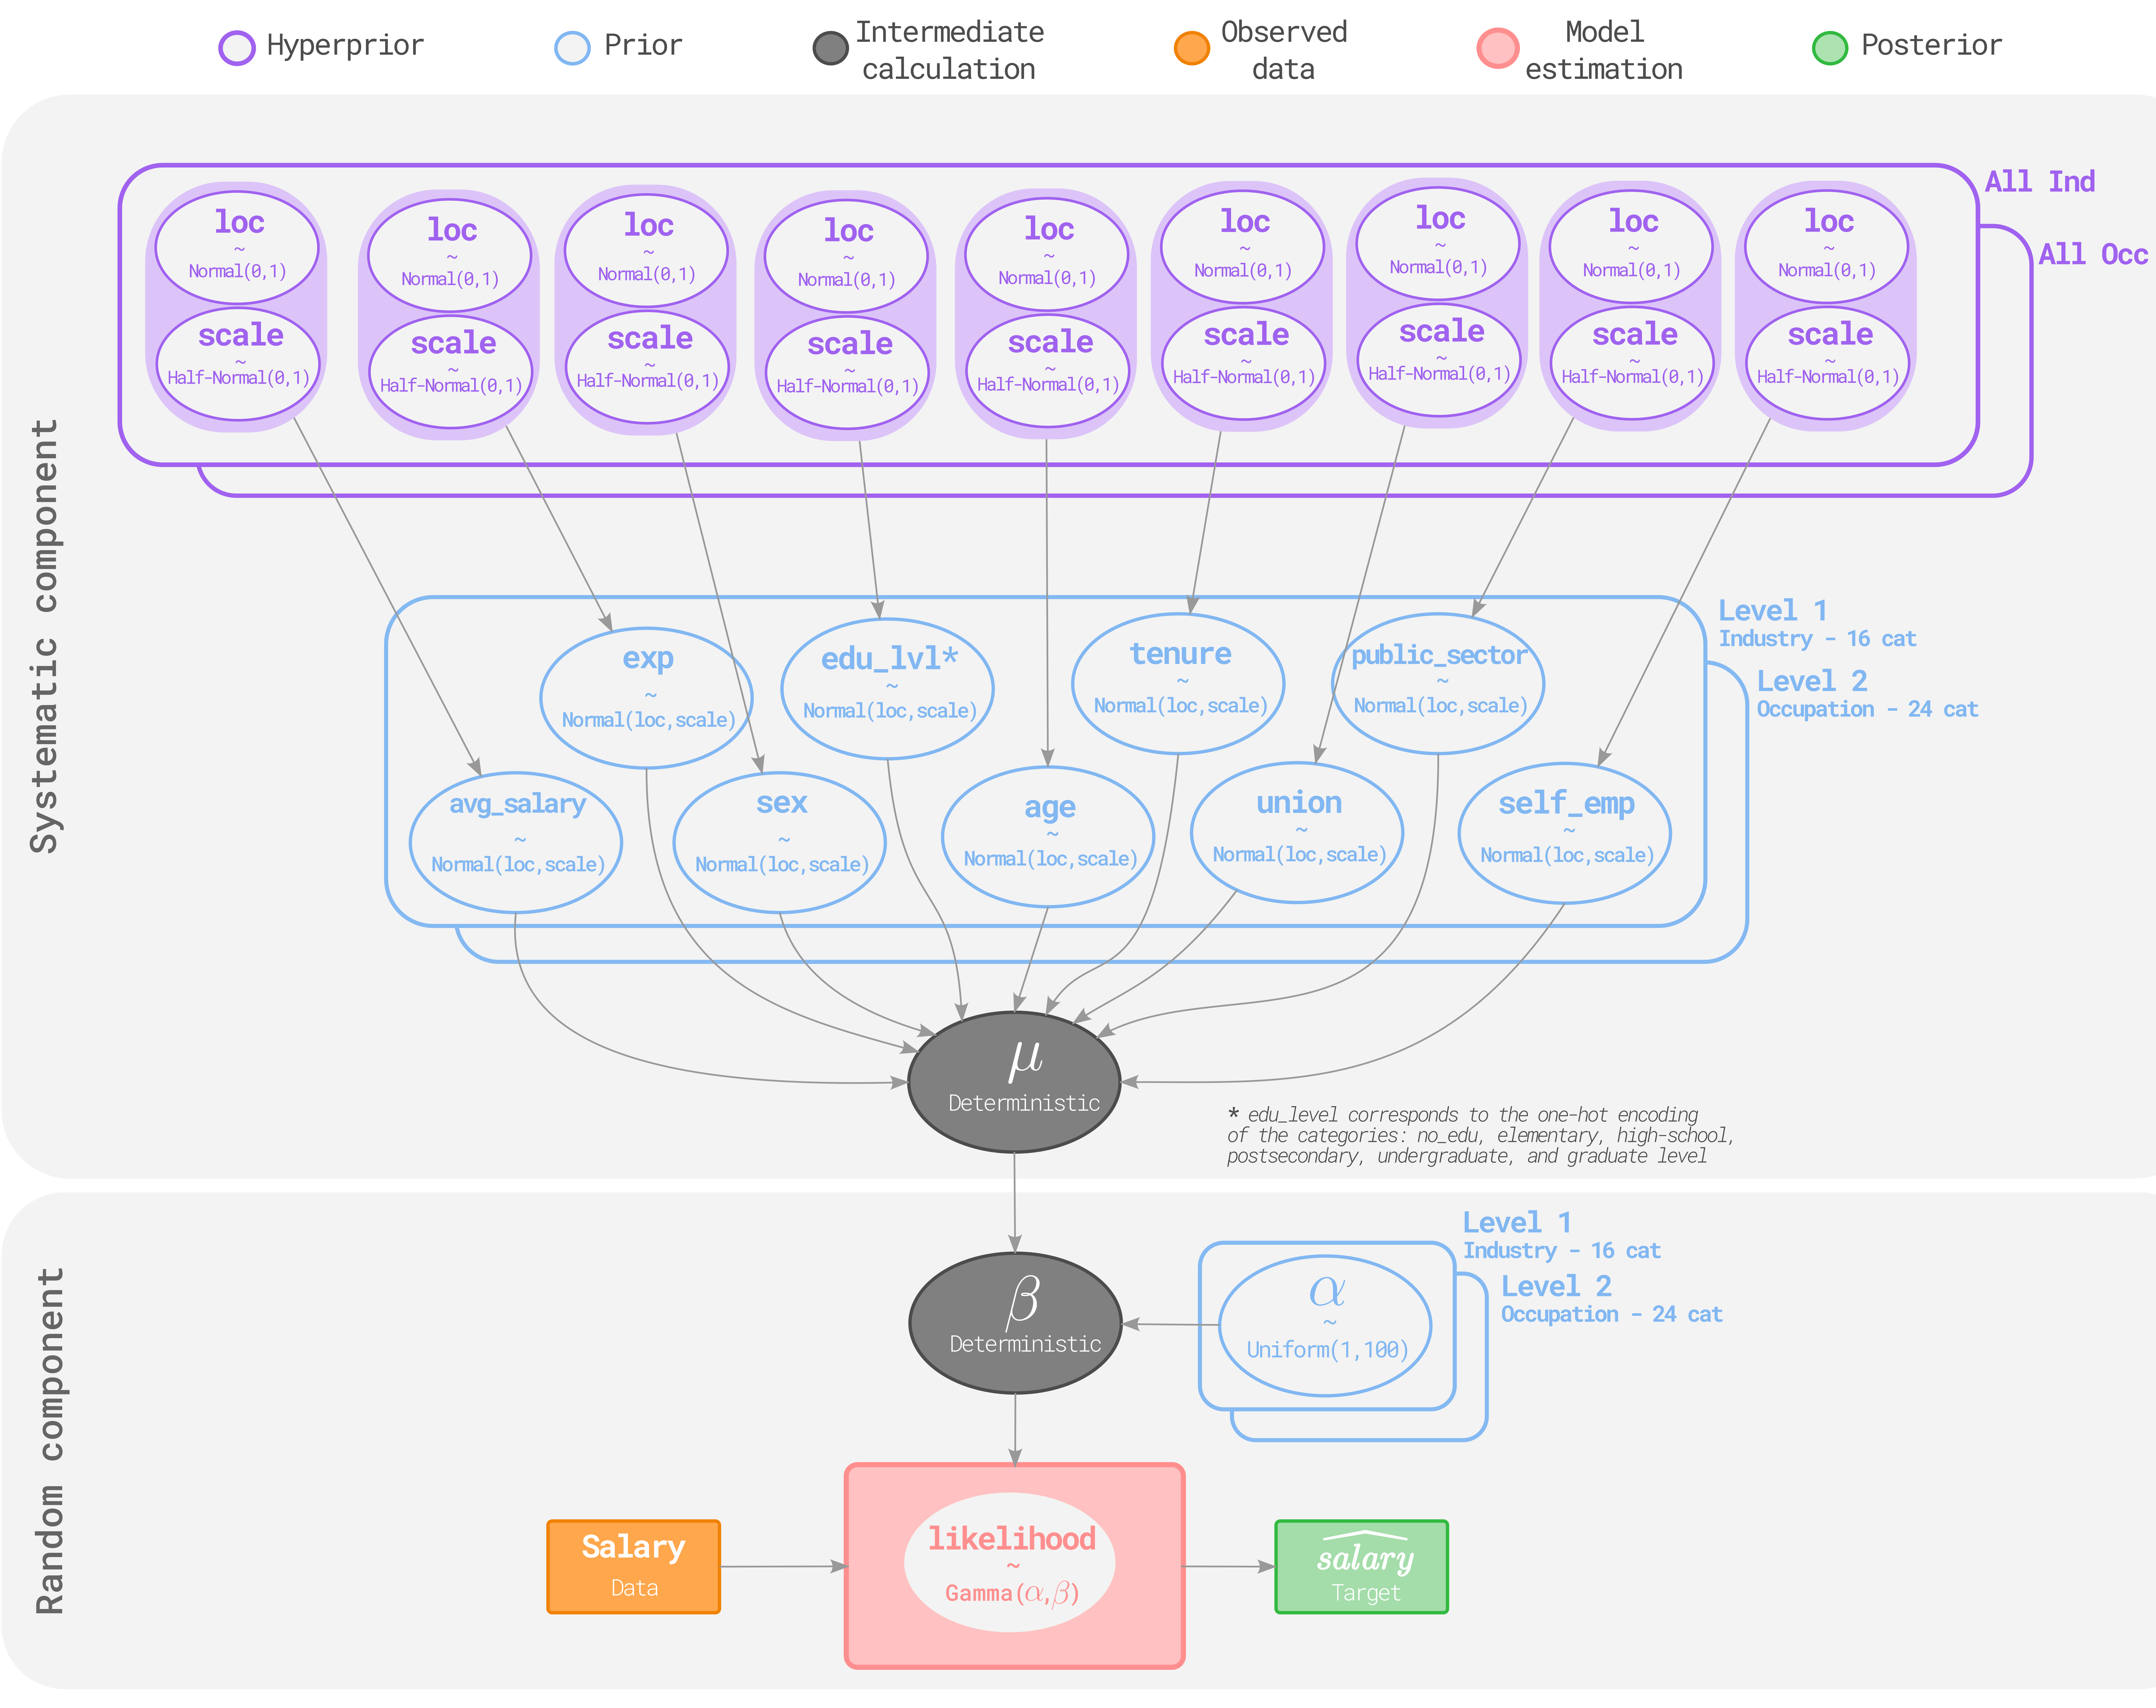
\includegraphics[width=0.96\textwidth]{images/ch5_hierarchical_graph/hierarchical_graph.png}
    \setlength{\abovecaptionskip}{-12pt}
    \caption{Model graph - Hierarchical}
    \label{fig:model_graph_hierarchical}
\end{figure}

\section{Model selection}\label{section:model_selection}

After running the inference on the three model structures, the results are compared using the performance metrics presented in \Cref{section:goodness_of_fit}. The model selection is divided into two sequential parts: 1) the model structure selection, which selects the best performing model between the pooled, no-pooled, and hierarchical structure, and 2) based on the structure selection, this part focuses on the most relevant variables based on model performance. The result from the 2-stage selection process is the optimal model, which is the proposal to replace the existing wage model in the labour market module of the ILUTE framework. 

\subsection{Structure selection: Pooled vs. No-pooled vs. Hierarchical model}\label{section:structure_selection} 

\Cref{fig:model_comparison} shows a model comparison using the LOO-CV measure (ELPPD score) and the WAIC score. The maximization of the ELPPD minimizes the KL divergence. Hence, in this figure, the higher the elppd value, the better the model.

\begin{figure}[H]
    \centering
    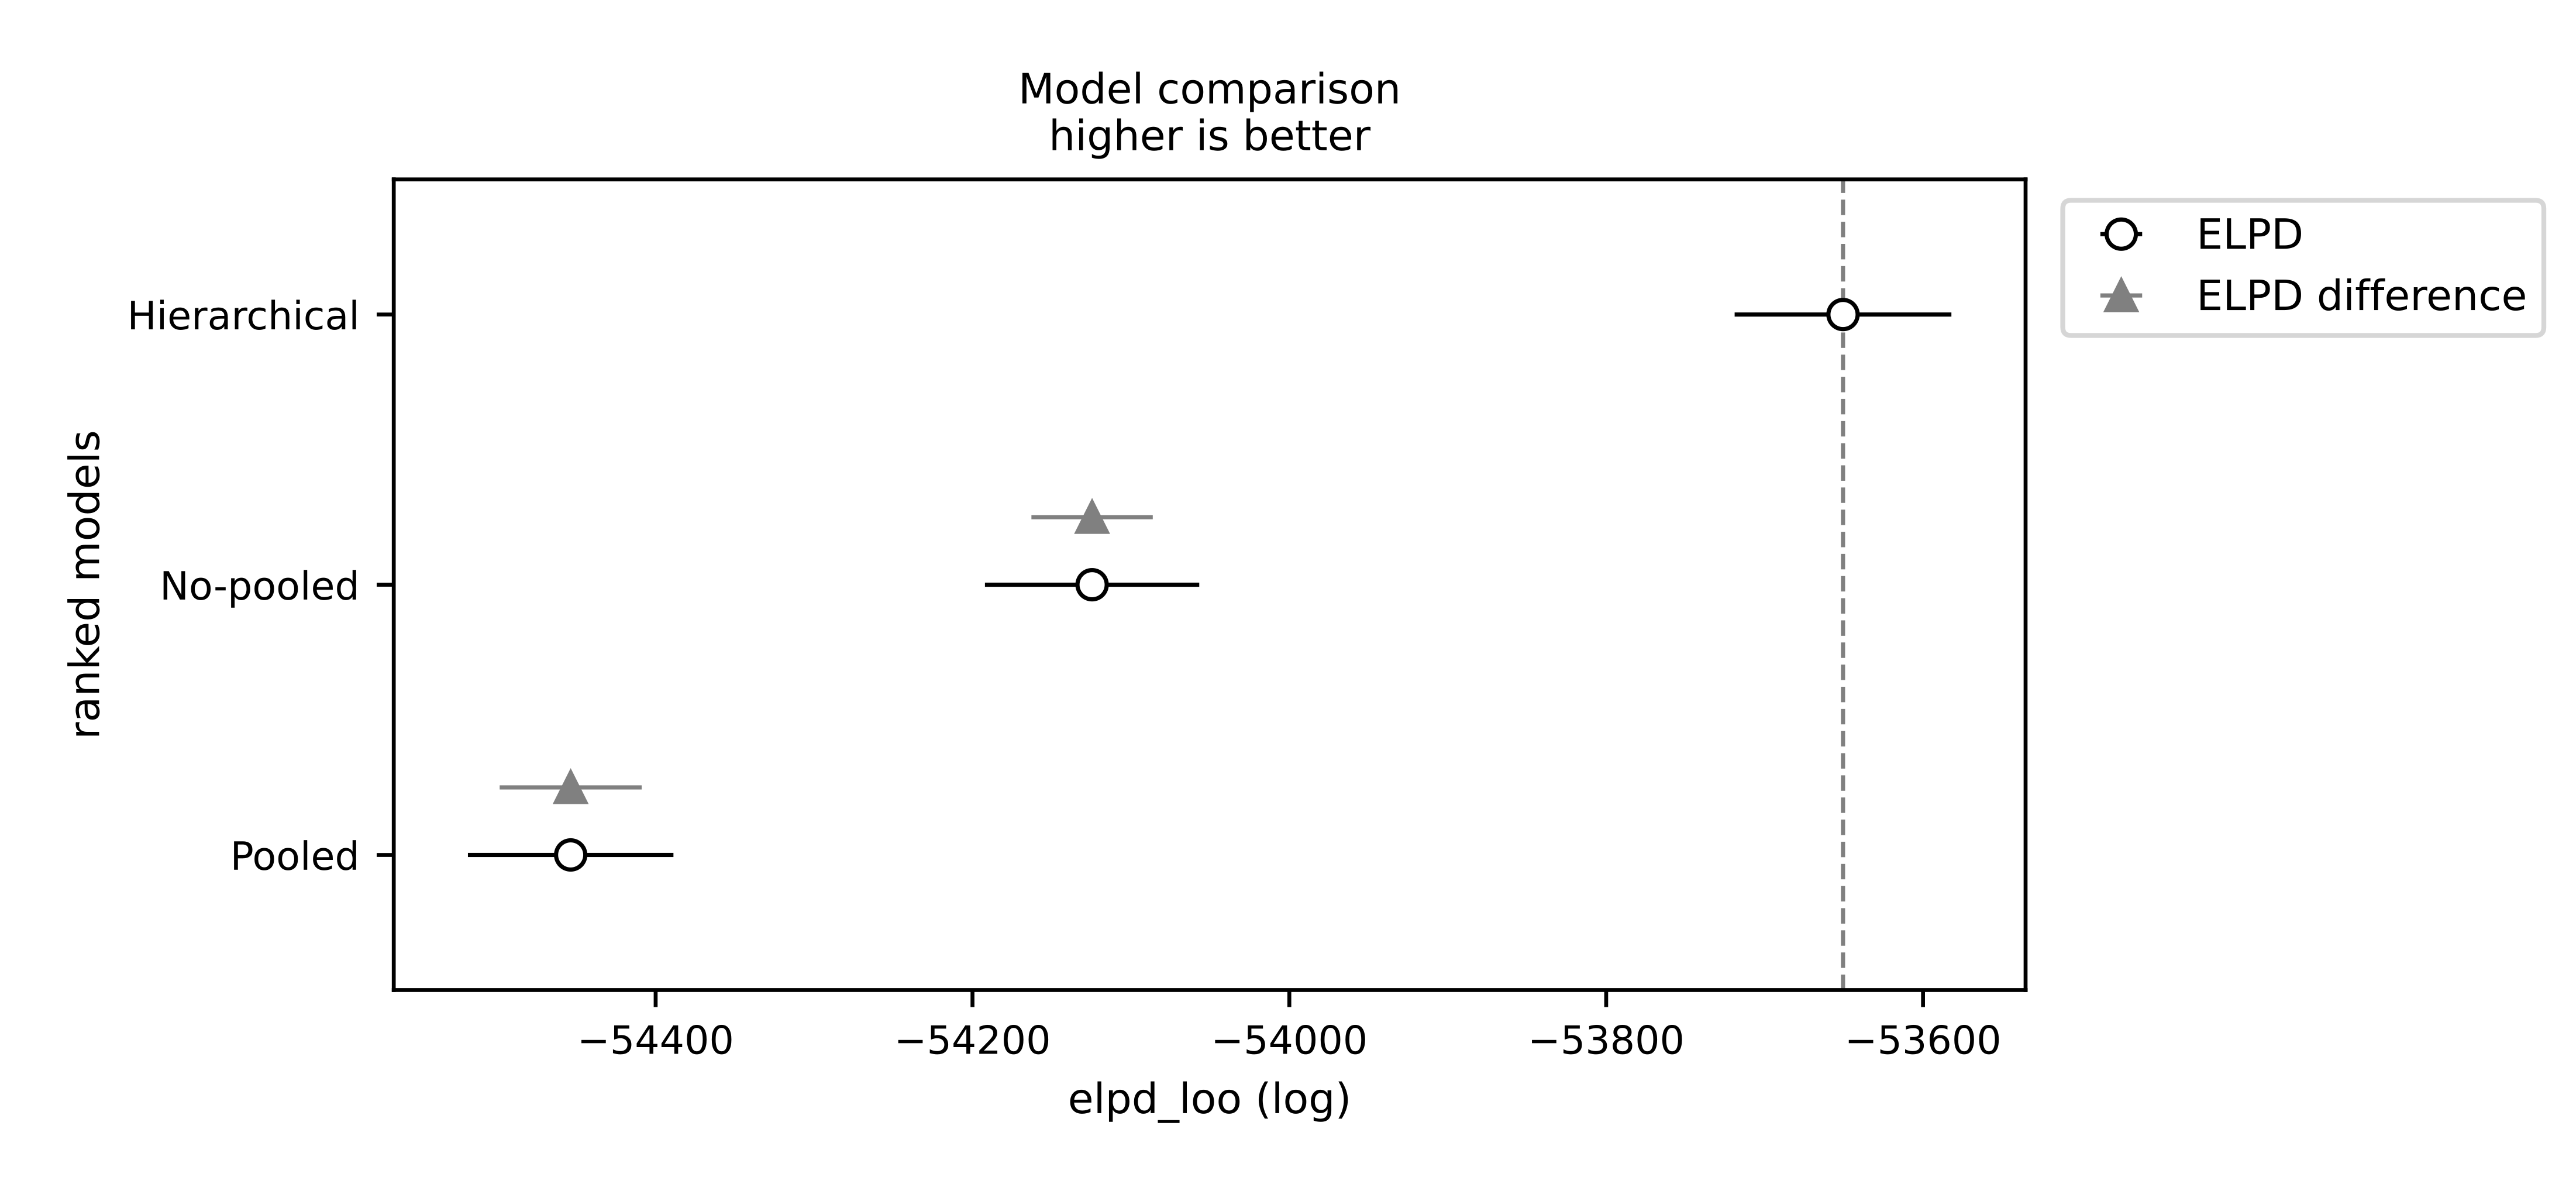
\includegraphics[width=0.96\textwidth]{images/ch5_model_structure_comparison/model_structure_comparison.png}
    \setlength{\abovecaptionskip}{-12pt}
    \caption{Model structure comparison }
    \label{fig:model_comparison}
\end{figure}

As expected, the hierarchical model shows better performance than the other approaches. The white circle represents the point estimate of the ELPPD-LOO score that measures the out-of-sample model performance. In contrast, the horizontal lines represent the uncertainty or error bars for the point estimate. Likewise, the ELPD difference provides a measure of comparison between each model and the reference model (best performant). The in-sample point estimate measures the model performance with the data used in the model estimation.  

The in-sample ELPPD score is an estimate of the performance of the training dataset. In contrast, the ELPPD-LOO score is an estimate of the performance on the validation dataset, which is a better estimate of the model performance in a real setting. The comparison between these two values ensures that the model is not overfitting. As expected, the model's performance in the in-sample case (training data) is higher than the out-of-sample case (validation data), which implies that the \textit{shrinkage effect} of the hierarchical approach is improving the performance by reducing the model complexity and avoiding overfitting. 

The results in \Cref{fig:model_comparison} confirm that the hierarchical structure provides a higher predictive power than the pooled and no-pooled approach. Including the hyperpriors allows the model to better capture the complex relationships and dependencies in the data compared to the other approaches (pooled and no-pooled). Therefore, from this point, all tests and additional runs are performed using the hierarchical structure.

\subsection{Forward variable selection} 

After selecting the optimal model structure, a Forward selection process is performed on the variables set to choose the most relevant from the predictive perspective. This process starts from the most straightforward model representation to the total variable set by adding one variable at each step. The simplest model corresponds to an intercept model (fixed effects), representing the average salary for that industry and that occupation. 

\Cref{fig:forward_selection} compares each variable addition from the simplest model to the one with the complete set of variables. These models are ranked from the best to the worst in terms of model performance, using the same ELPPD-LOO and WAIC scores used in the model structure selection.

\begin{figure}[H]
    \centering
    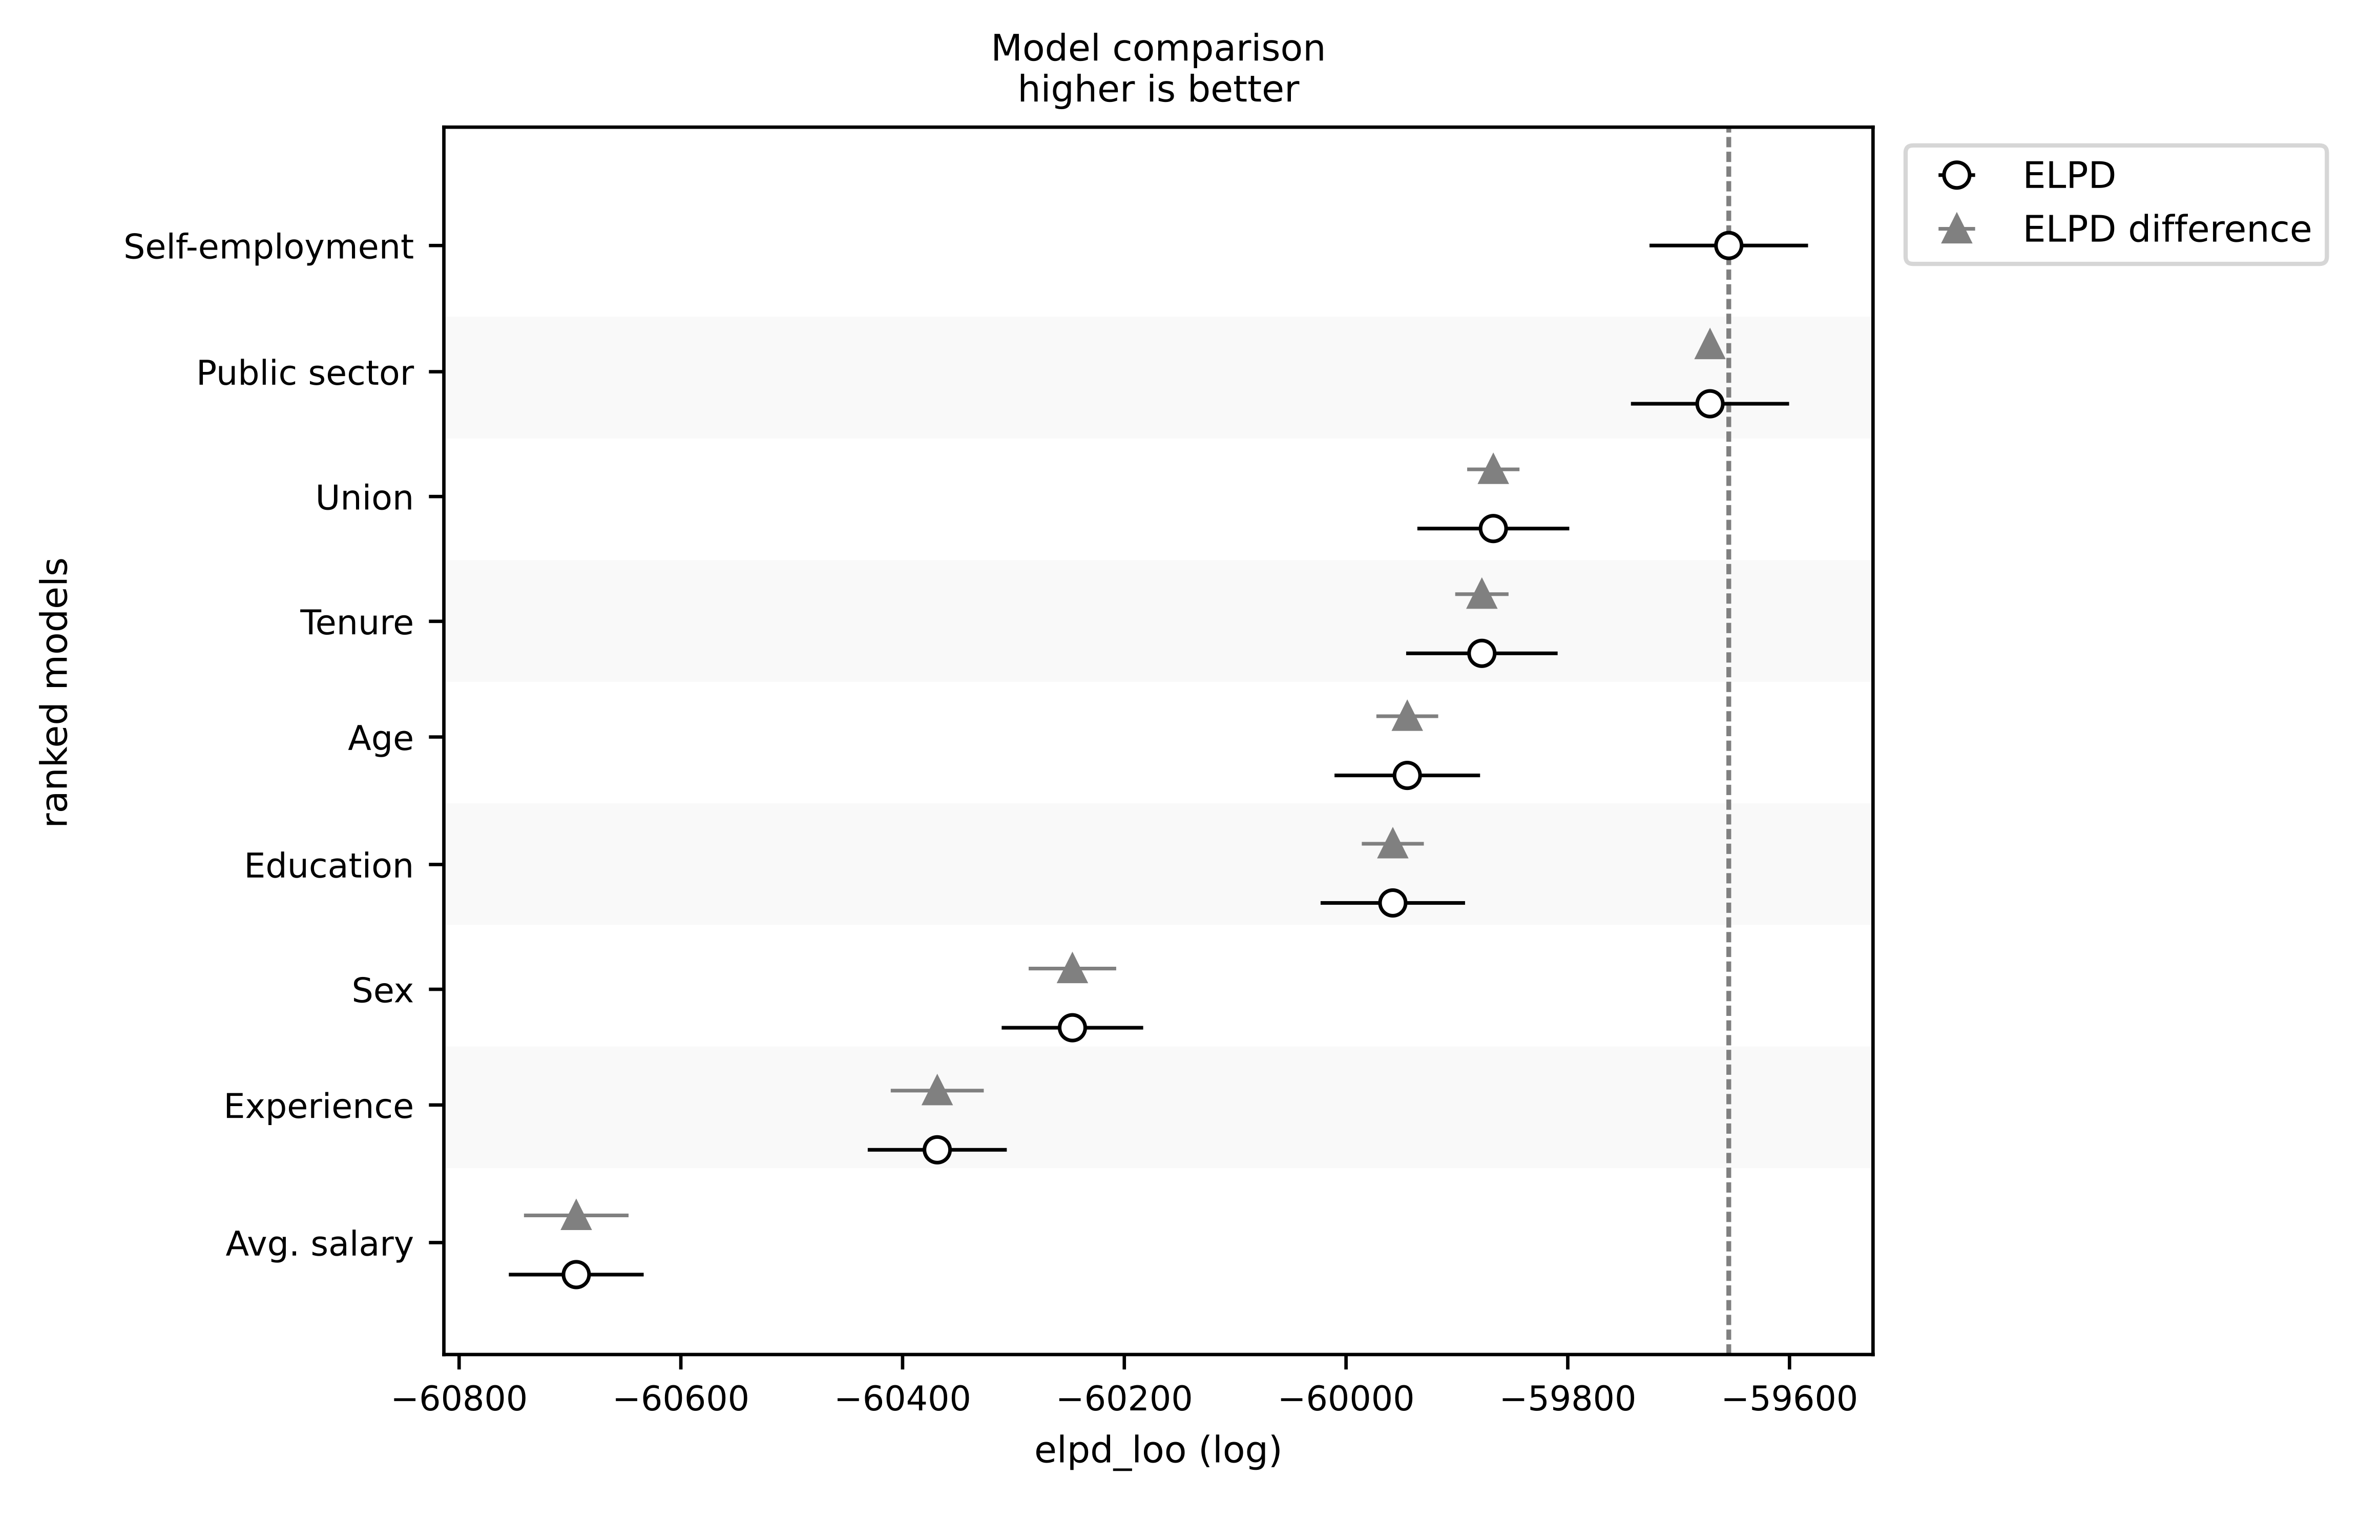
\includegraphics[width=0.8\textwidth]{images/ch5_forward_sel/forward_sel.png}
    \setlength{\abovecaptionskip}{-5pt}
    \caption{Forward variable selection}
    \label{fig:forward_selection}
\end{figure}

Starting from the intercept (avg\_salary), each variable is added to the model and the \textit{elpd} measure is calculated. Although adding each variable improves the model performance, the variables with the most significant effect on the target variable are experience, sex, education, and employment sector. These results are in line with the theoretical models and the literature review. On the other hand, variables such as age, tenure, and self-employment add little or no information at all, so they can be dropped from the model without losing significant performance. This selection process helps to reduce the model complexity and reduces the risk of overfitting the data.

Based on this variable selection process, the optimal model contains the predictors: \textbf{\textit{Avg\_salary, Experience, Sex, Education, Union and Public Sector}}. \Cref{fig:final_posterior} shows a subset of the posterior distributions for some industries and occupations in the final model. The chart with all model parameters is presented in \Cref{app:posterior_dists_final}.

\begin{figure}[H]
    \centering
    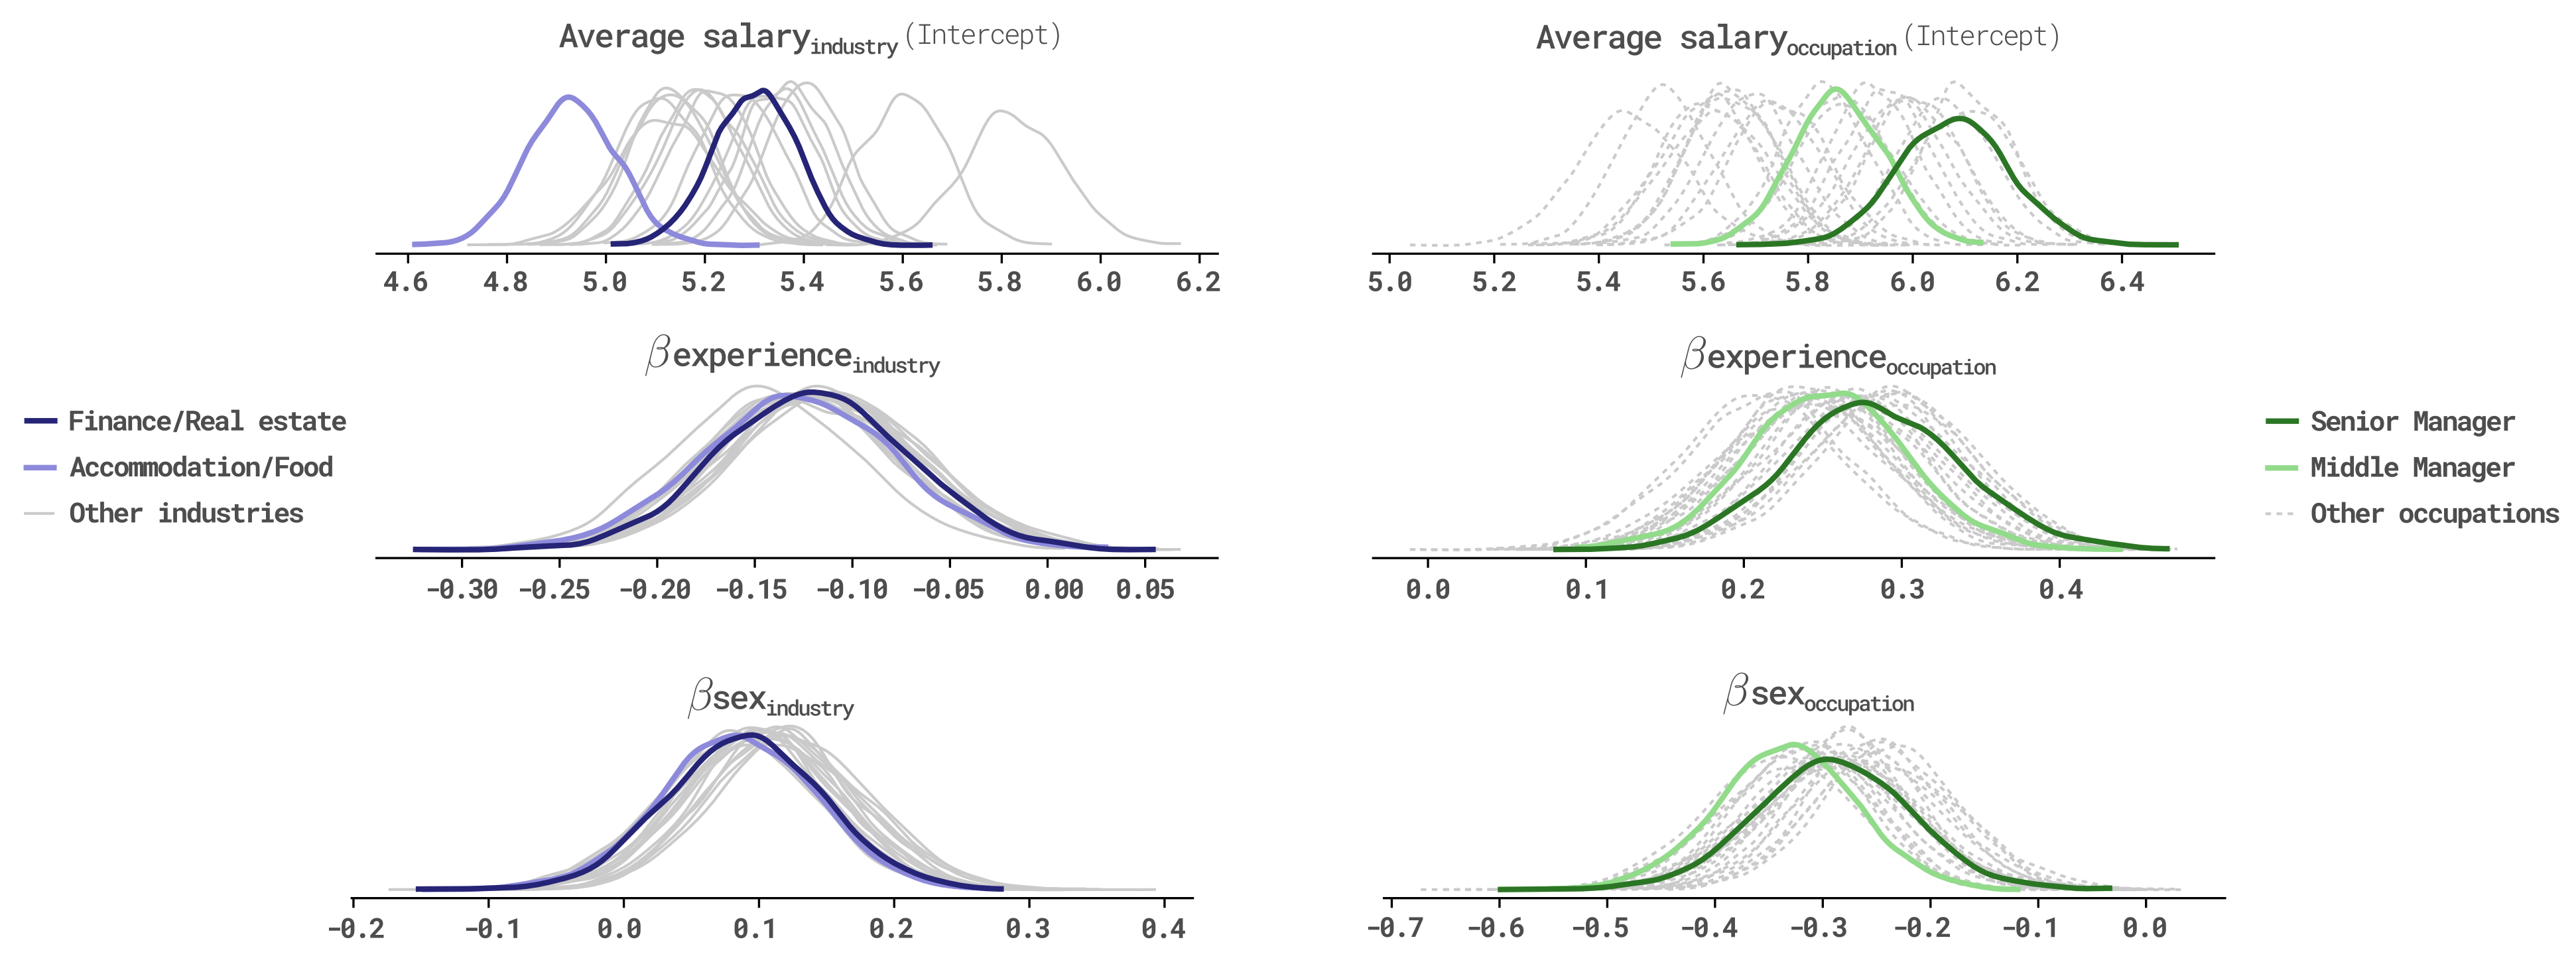
\includegraphics[width=1.0\textwidth]{images/ch5_traces/trace_1.png}
    \setlength{\abovecaptionskip}{-5pt}
    \caption{Posterior distributions for some industries and occupations in the final model}
    \label{fig:final_posterior}
\end{figure}

\section{Model interpretability}

The following bullets discuss the main results based on the posterior parameter distributions obtained from the Optimal model (after forward selection). It is important to highlight that although these results are in line with theory, they reflect the cultural and societal conditions from 1996 to 2007: 

\begin{itemize}
    \item Given that the Gamma GLM uses a log-link function, the relationship between the model parameters and the target variable is multiplicative\footnote{After applying the inverse of the log-link (exponential), which converts the value to the units of the data (CAD 2023)}. Therefore, the intercept (avg\_salary by industry and occupation) is interpreted as the base salary. Then, each parameter increases or reduces by a certain percentage of this salary base according to their effect (positive or negative)\footnote{After applying the inverse of the log-link (exponential)}. 

    \item As expected, most of the salary variability comes from the industry and occupation category, given the hierarchical structure of the labour market. In particular, the salaries of individuals in some physically demanding occupations (e.g. Construction trades) are explained mainly by their occupation rather than by the industry. This means this occupation has a low industry-base salary but higher occupation-base salaries than the other industries and occupations. 
    
    \item The gender gap is mainly explained by the negative values of the sex parameter related with occupation. Although this parameter is positive for industry level, when considering the overall effect (considering both industry and occupation value) the difference is negative for all industries and occupations. 
    
    \item Based on the forward selection results and the magnitude of the parameters, education level is the predictor that contributes the most to the variability explanation. As supported by the human capital theory, education is positively correlated with salaries across all industries and occupations. 
    
    \item Experience is a better predictor of salaries than job tenure because the latter is attached to the current job. Conversely, experience can be seen as a proxy for the skill set of an individual. Therefore, it provides more information about the potential salary of a candidate. 
    
    \item According to the model, public sector and union participation positively correlate with salaries. As public employees and unions can have more bargaining capacity, this could benefit the individuals in this sector and under union agreements. 
\end{itemize}

\section{Online learning: Longitudinal analysis of the estimated parameters }

Labour markets are constantly evolving. Some changes are observed in short periods, usually cyclical and related to the oscillation between supply and demand. In contrast, some changes are observed in more extended periods, usually related to technological, social, or political changes. The former is more straightforward to predict, while the latter is challenging because it usually corresponds to structural changes. Given the effect of the long-term changes in the labour market structure, the evolution of the model parameters through time becomes relevant for measuring the model validity and robustness to structural changes. 

The model performance can be assessed through time by comparing the estimated parameters using the whole dataset versus the estimated parameters using a sequential approach. This sequential estimation is aligned with the Bayesian inference framework because the posterior belief on the current period can become the prior belief for the next period. This approach is called \textit{Online learning}. 

Using the hierarchical model after the variable selection, \Cref{fig:online_learning_salary} to \Cref{fig:online_learning_sex} compare the evolution of the posterior distribution for some model parameters using Online Learning and the same parameter posterior distributions estimated with the whole dataset. 

\begin{figure}[H]
    \centering
    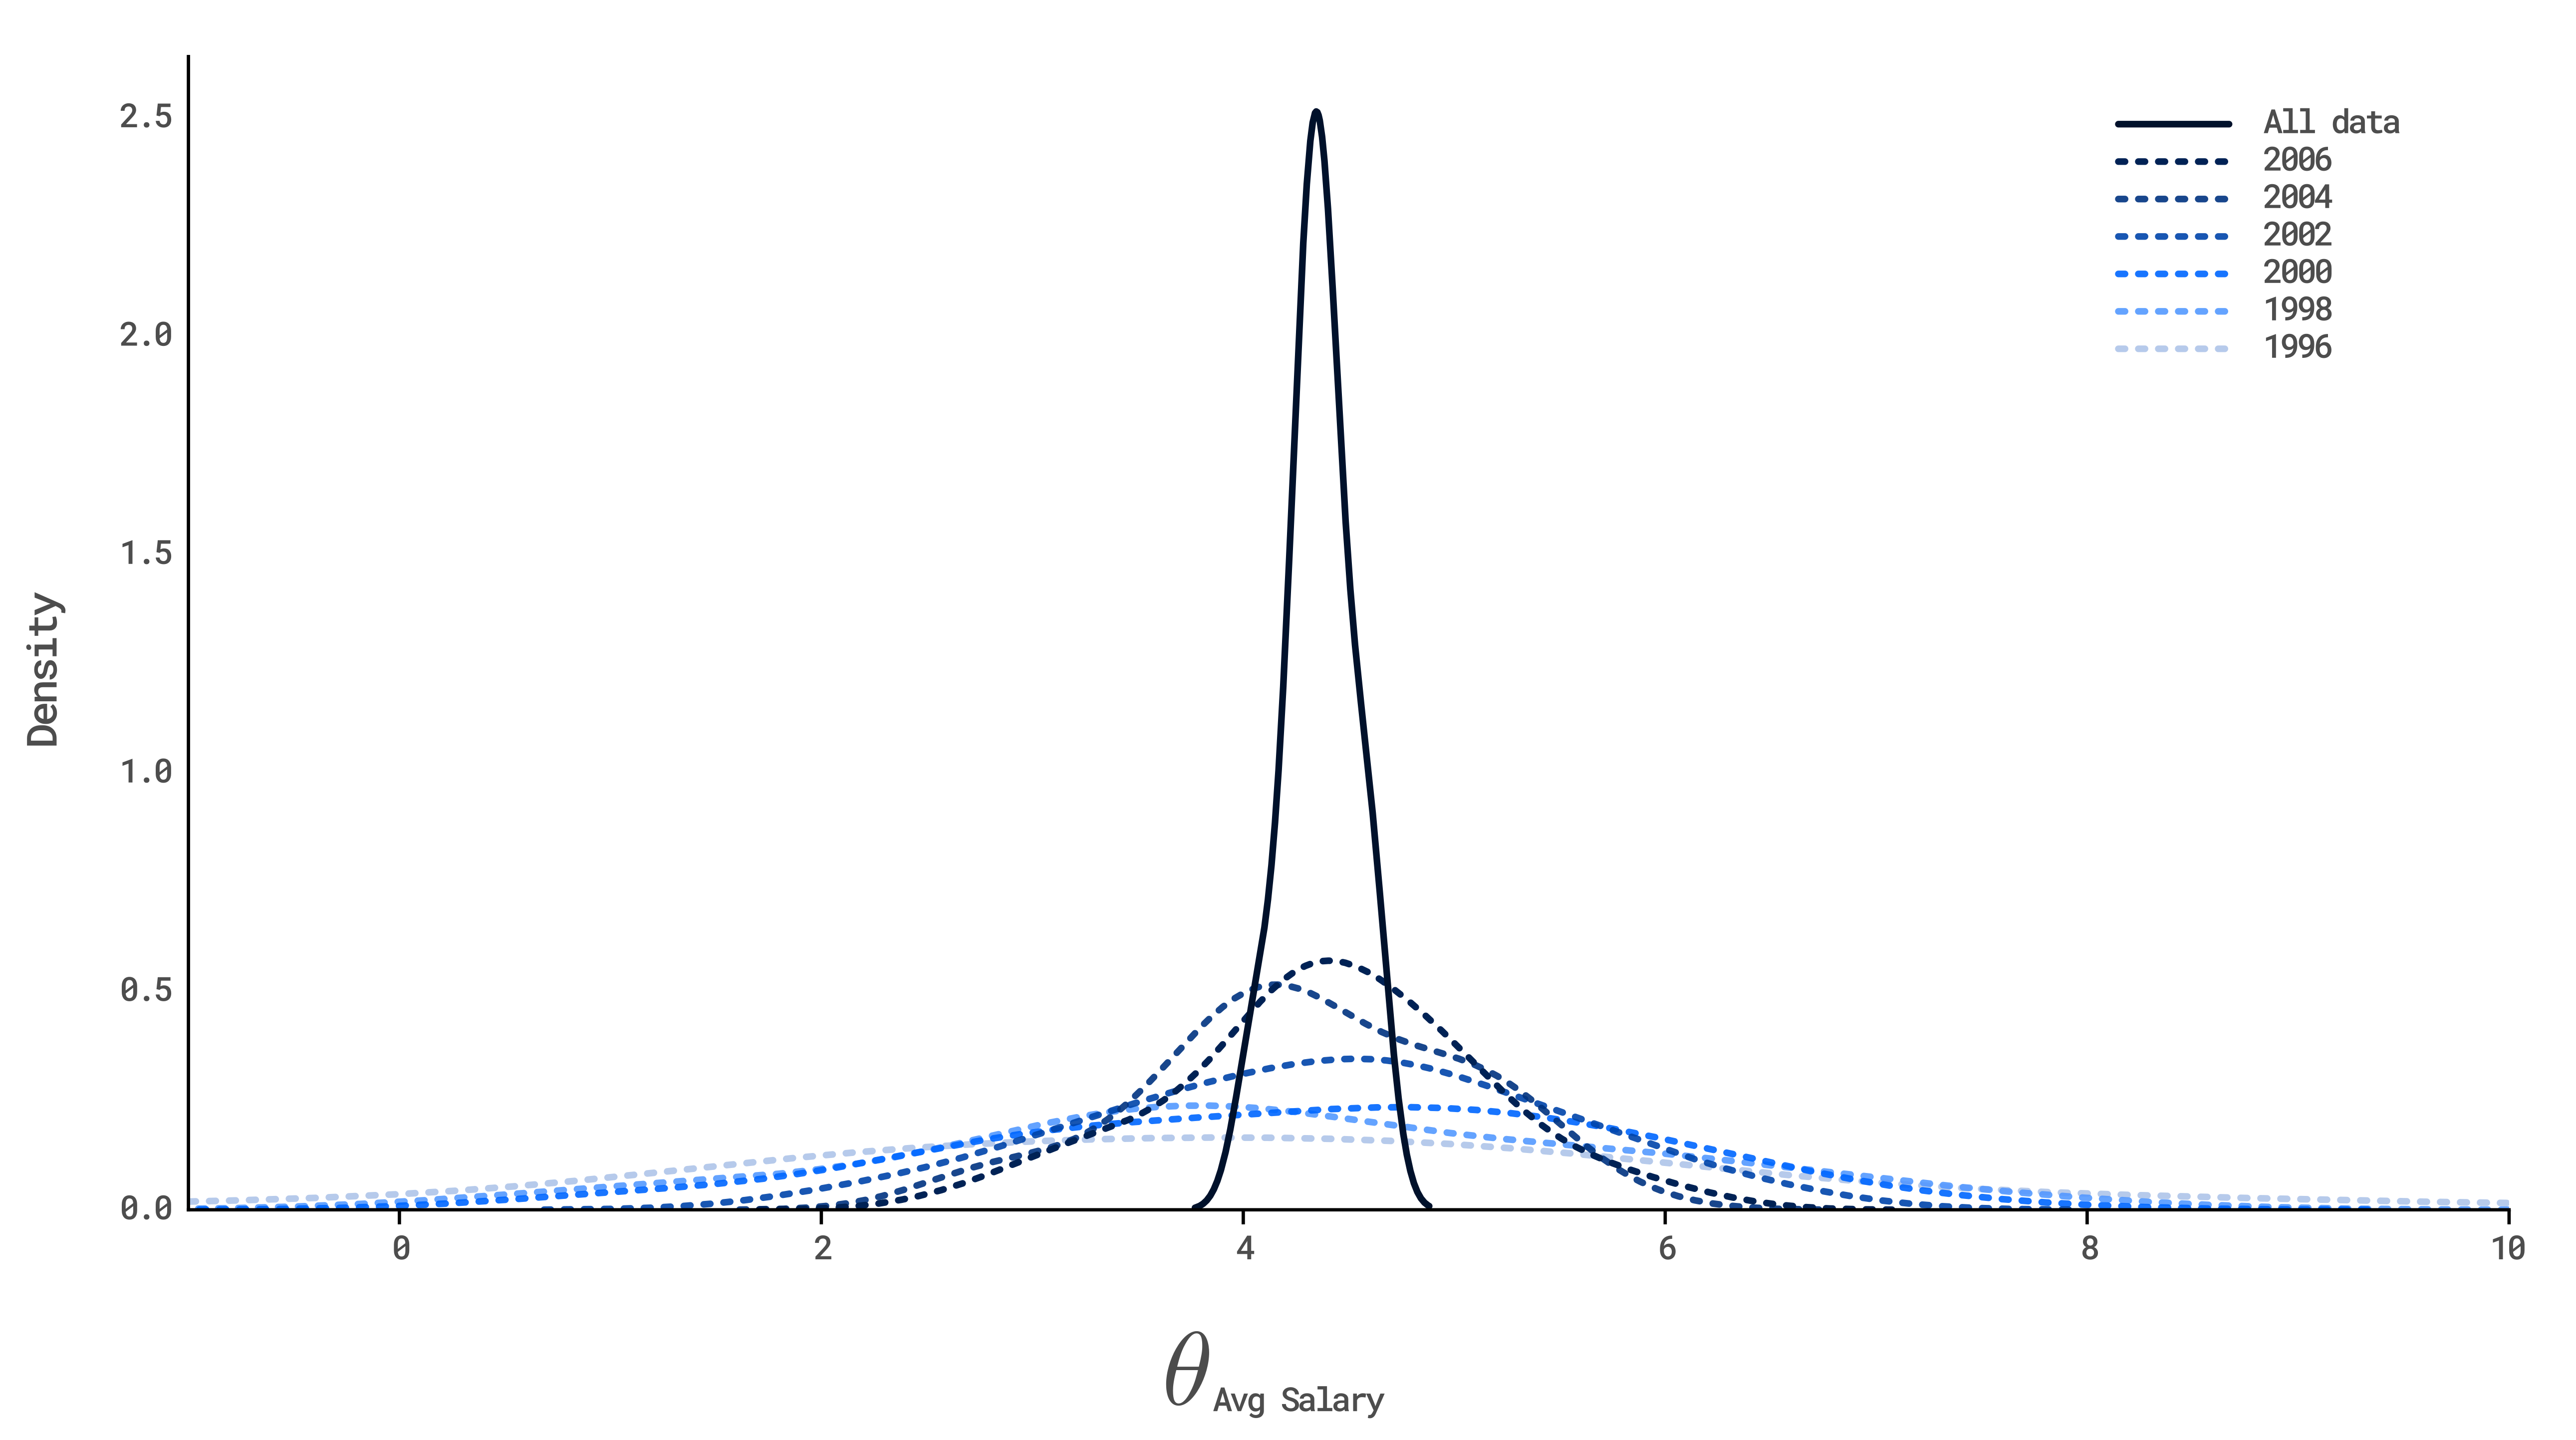
\includegraphics[width=0.75\textwidth]{images/ch5_online_learning/online_learning_salary.png}
    \setlength{\abovecaptionskip}{-10pt}
    \caption{Longitudinal analysis for model parameter - Avg. Salary (Intercept)}
    \label{fig:online_learning_salary}
\end{figure}

\begin{figure}[H]
    \centering
    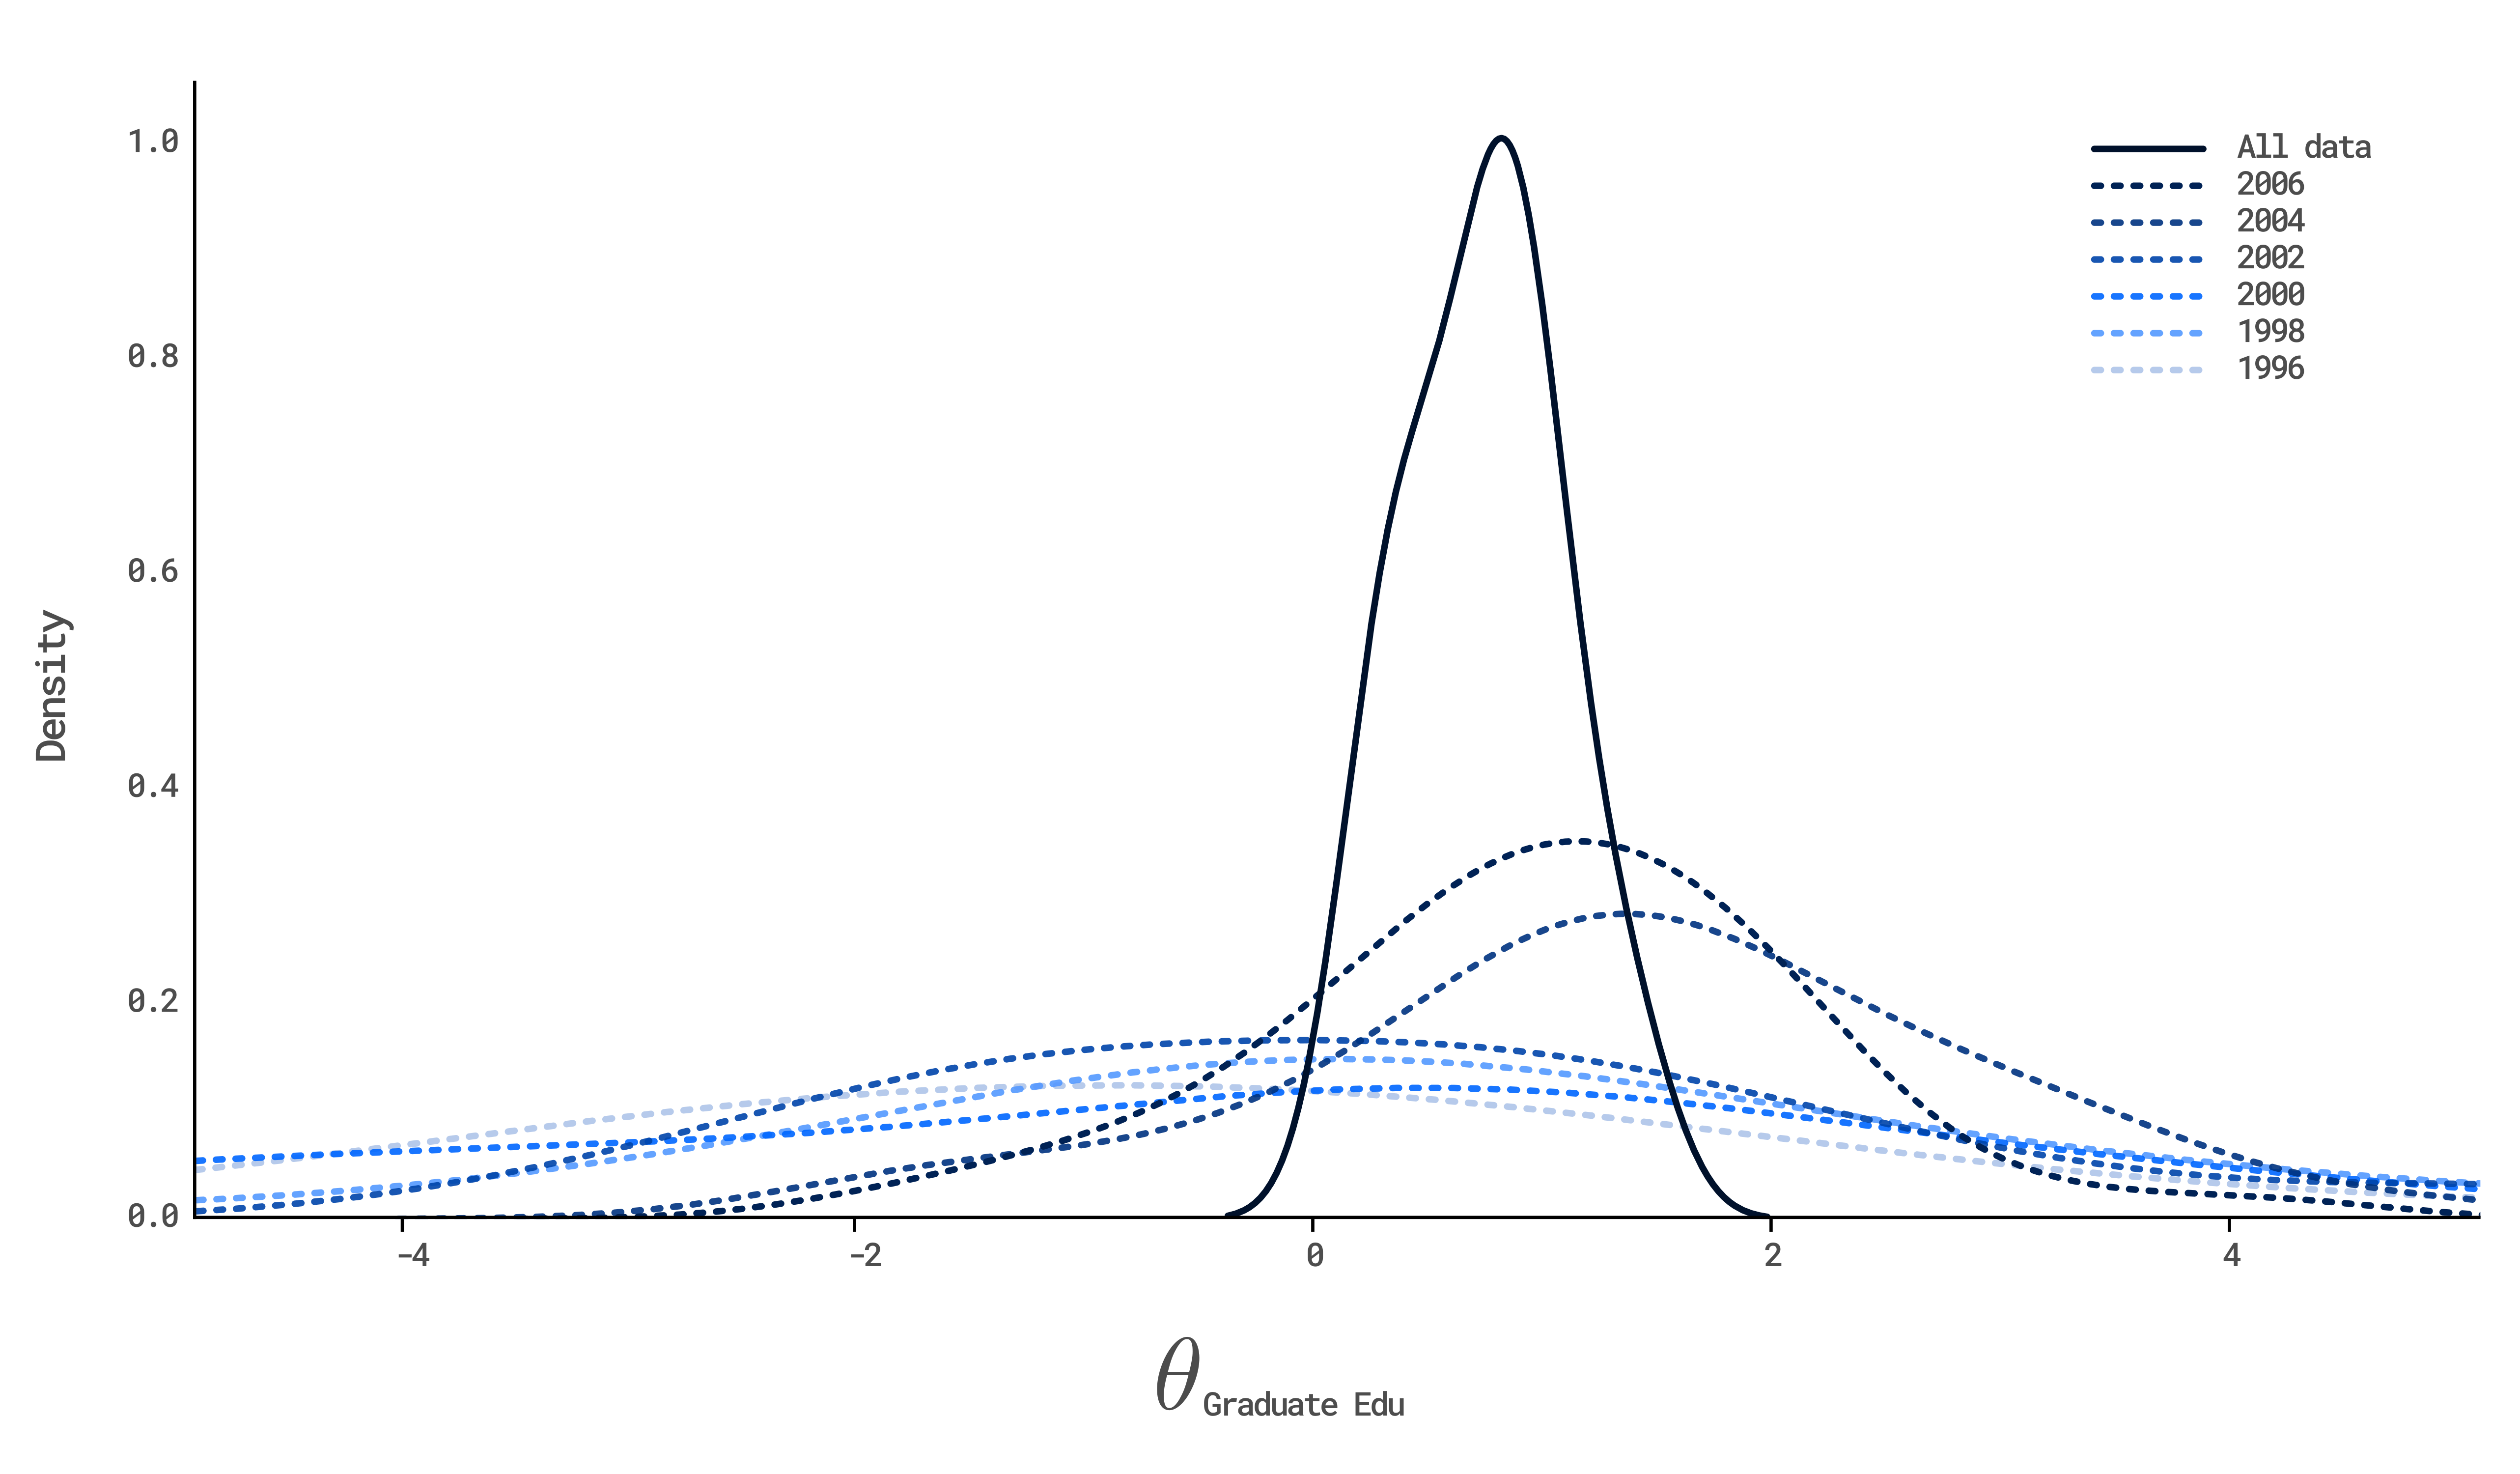
\includegraphics[width=0.8\textwidth]{images/ch5_online_learning/online_learning_grad.png}
    \caption{Longitudinal analysis for model parameter - Graduate Education Level }
    \label{fig:online_learning_grad}
\end{figure}

\begin{figure}[H]
    \centering
    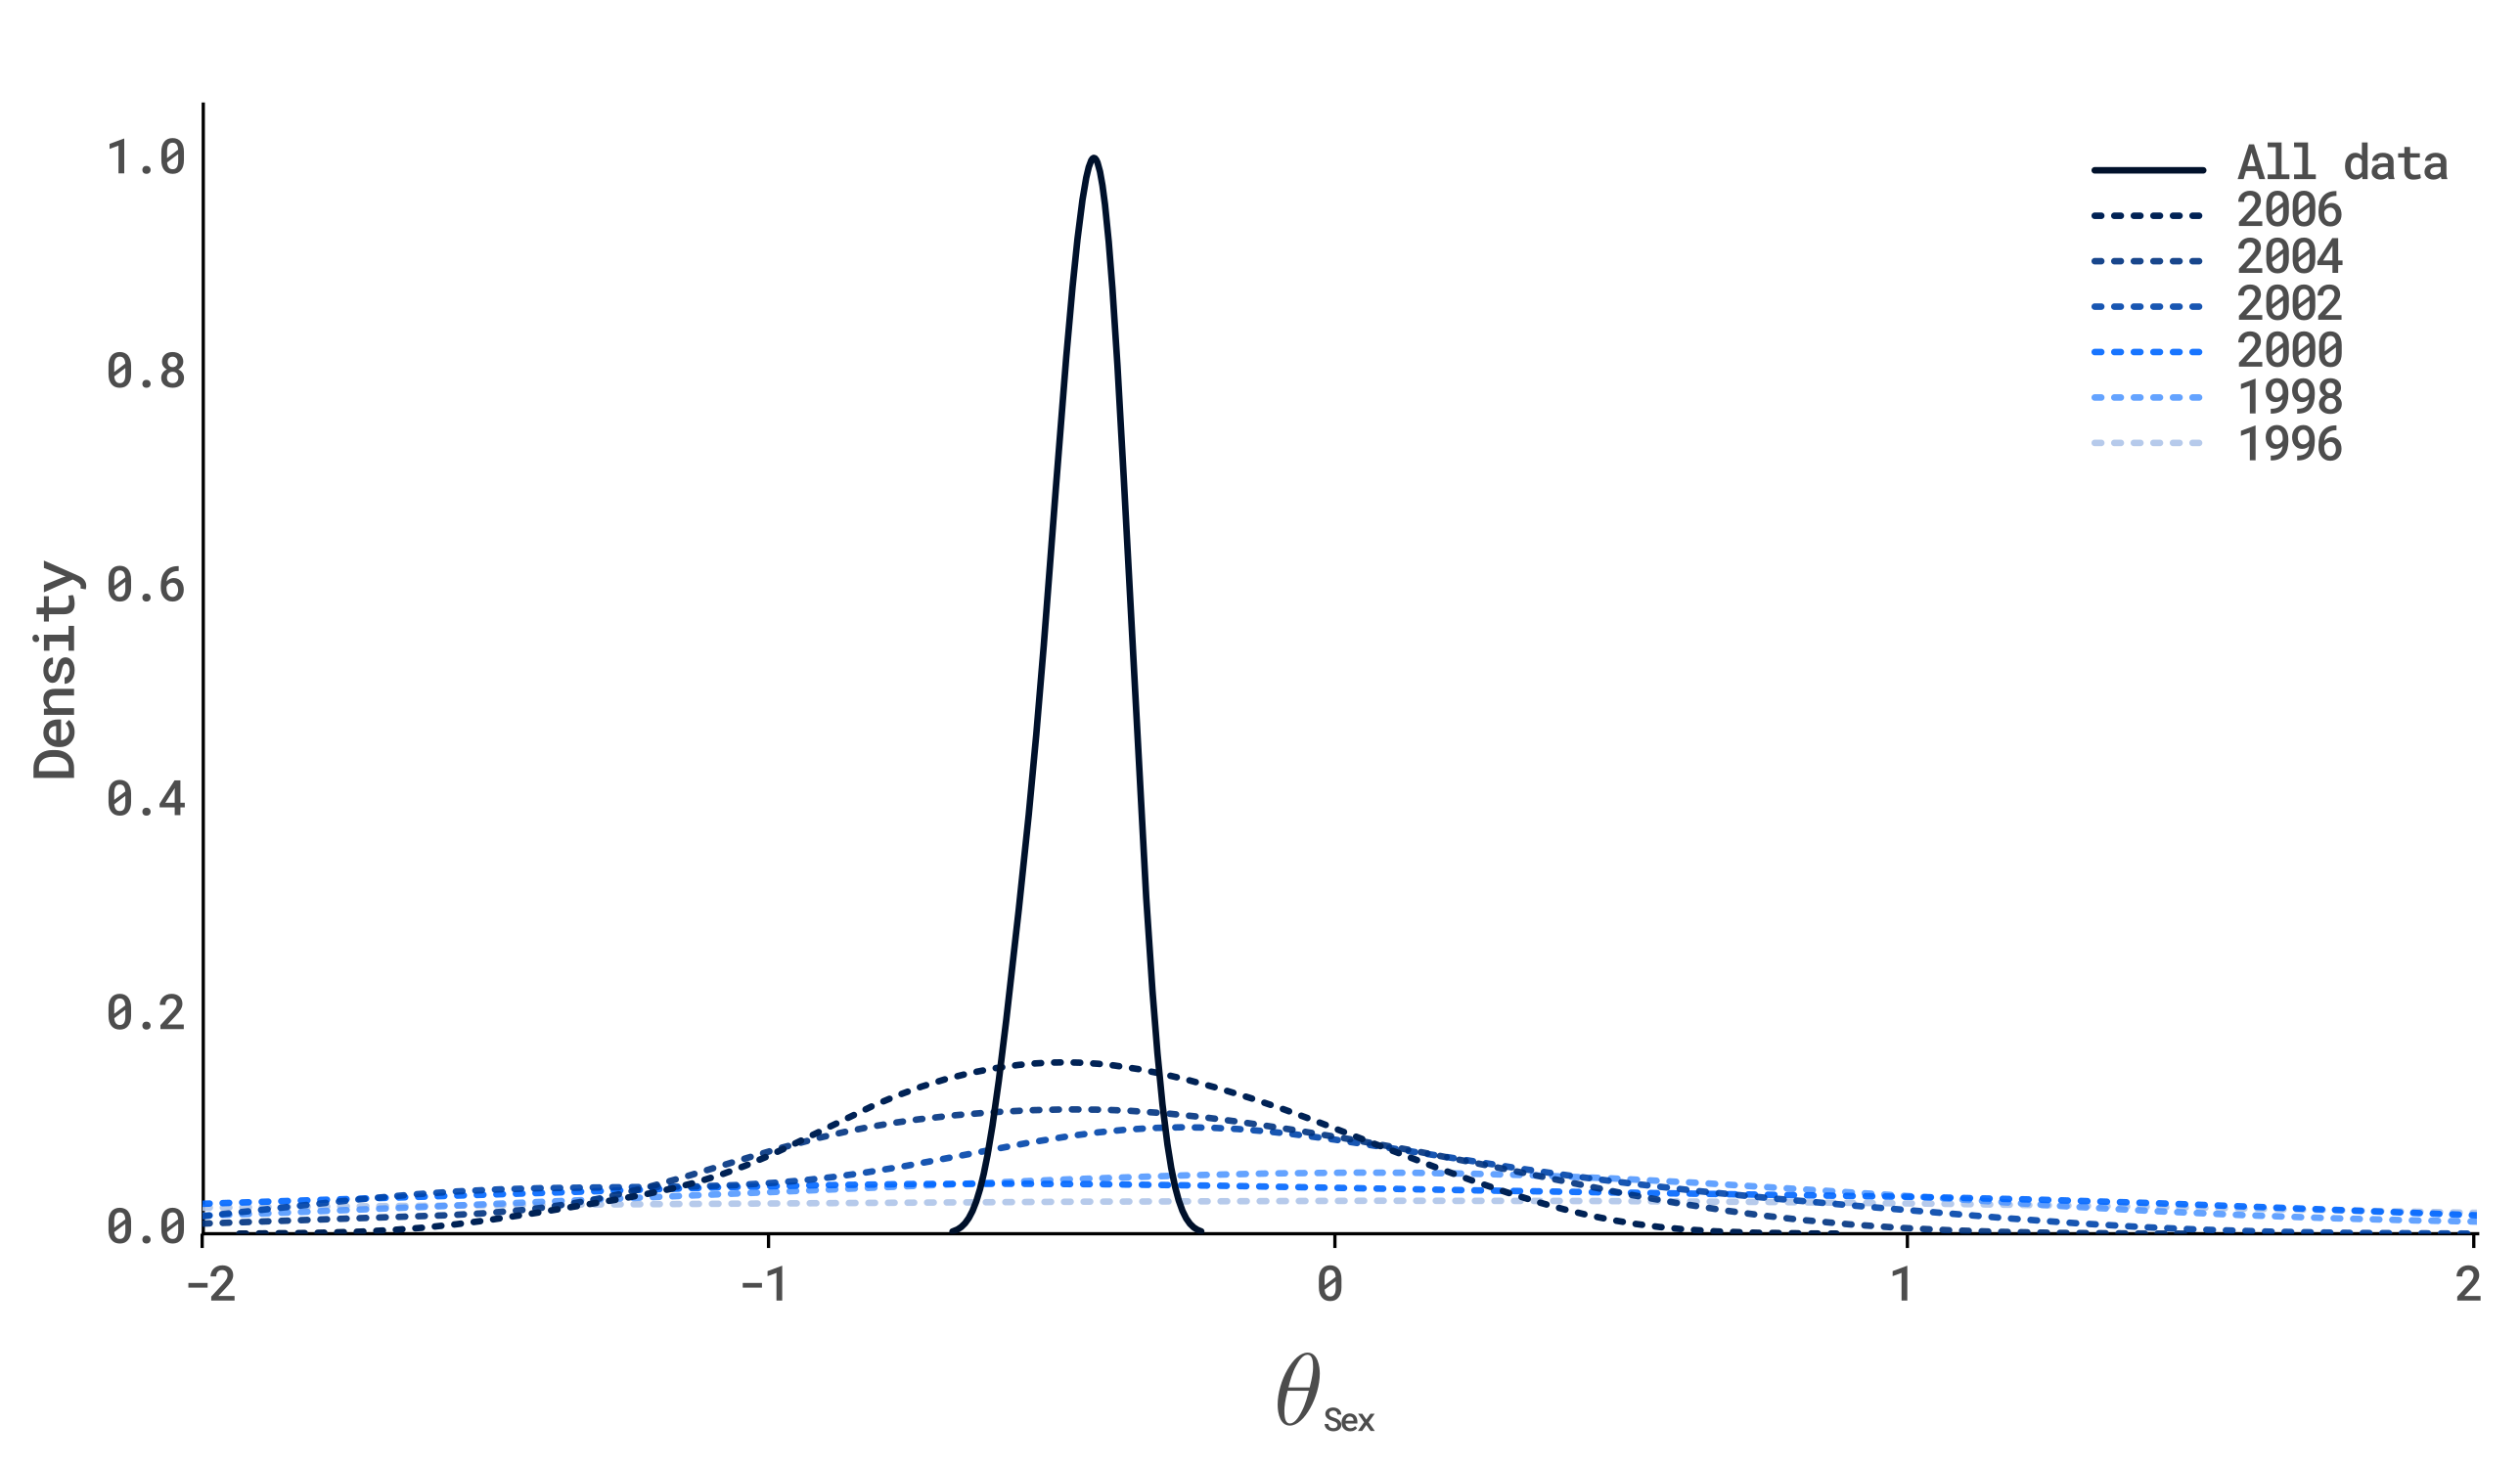
\includegraphics[width=0.8\textwidth]{images/ch5_online_learning/online_learning_gender.png}
    \caption{Longitudinal analysis for model parameter - Sex }
    \label{fig:online_learning_sex}
\end{figure}

The longitudinal analysis shows how the posterior distribution of each parameter is updated sequentially in light of new data. Starting from 1996, the priors are located at 0 for all model parameters, but the posteriors move towards the actual value each year. In the case of Average salary and Graduate level, they move positively, whereas in the case of Sex, they move negatively. As more data are available, the posterior distribution starts peaking around the true value, implying that the model is getting more confident in the parameter estimation. When comparing the posteriors using the whole dataset versus the sequential update (online learning), there is a difference in the density value. However, the peak of both scenarios is at the same point, which demonstrates that the Online learning setting produces reasonable estimates with a smaller dataset. 

Therefore, the Online Learning technique also allows an easy and natural way to update the model parameters because it resembles how data are generated. Also, the model is more robust to structural changes because it combines the past and current structure with the trend changes in the labour market. It requires less data and computational power because the estimation task is performed gradually. 
   
\section{Model validation}\label{section:model_validation}

While the in-sample metrics provide a general idea of how well the model fits the existing data, the out-of-sample performance measures the model's capability to generalize in the light of new data. That generalization determines whether the model captures the complex relationships between the model variables and ensures that the model does not “memorize” the noise in the data. Therefore, the out-of-sample evaluation assess the model's performance in a real setting. 

A graphical comparison between the true and the estimated salary distribution for the validation dataset is carried out to visually assess the potential use of the predicted distributions in a simulation setting, such as the labour market module in the ILUTE framework. This validation is performed in two levels: the aggregated that ensures the model is correctly representing salaries within different clusters observed in the data (e.g. salary distribution by industry, occupation, gender, and education level, among others) and the disaggregated that ensures the salary is being correctly predicted for each worker given their attributes.

\subsection{Aggregated level} 

The following charts show a comparison between the true salary distribution and the predicted salary distribution for different group variables, being industry and occupation, the most relevant groups given the hierarchical structure of the labour market. From these figures, it is observed that the model adequately represents the salary across all group variables regarding their shape and values.

\begin{figure}[H]
    \centering
    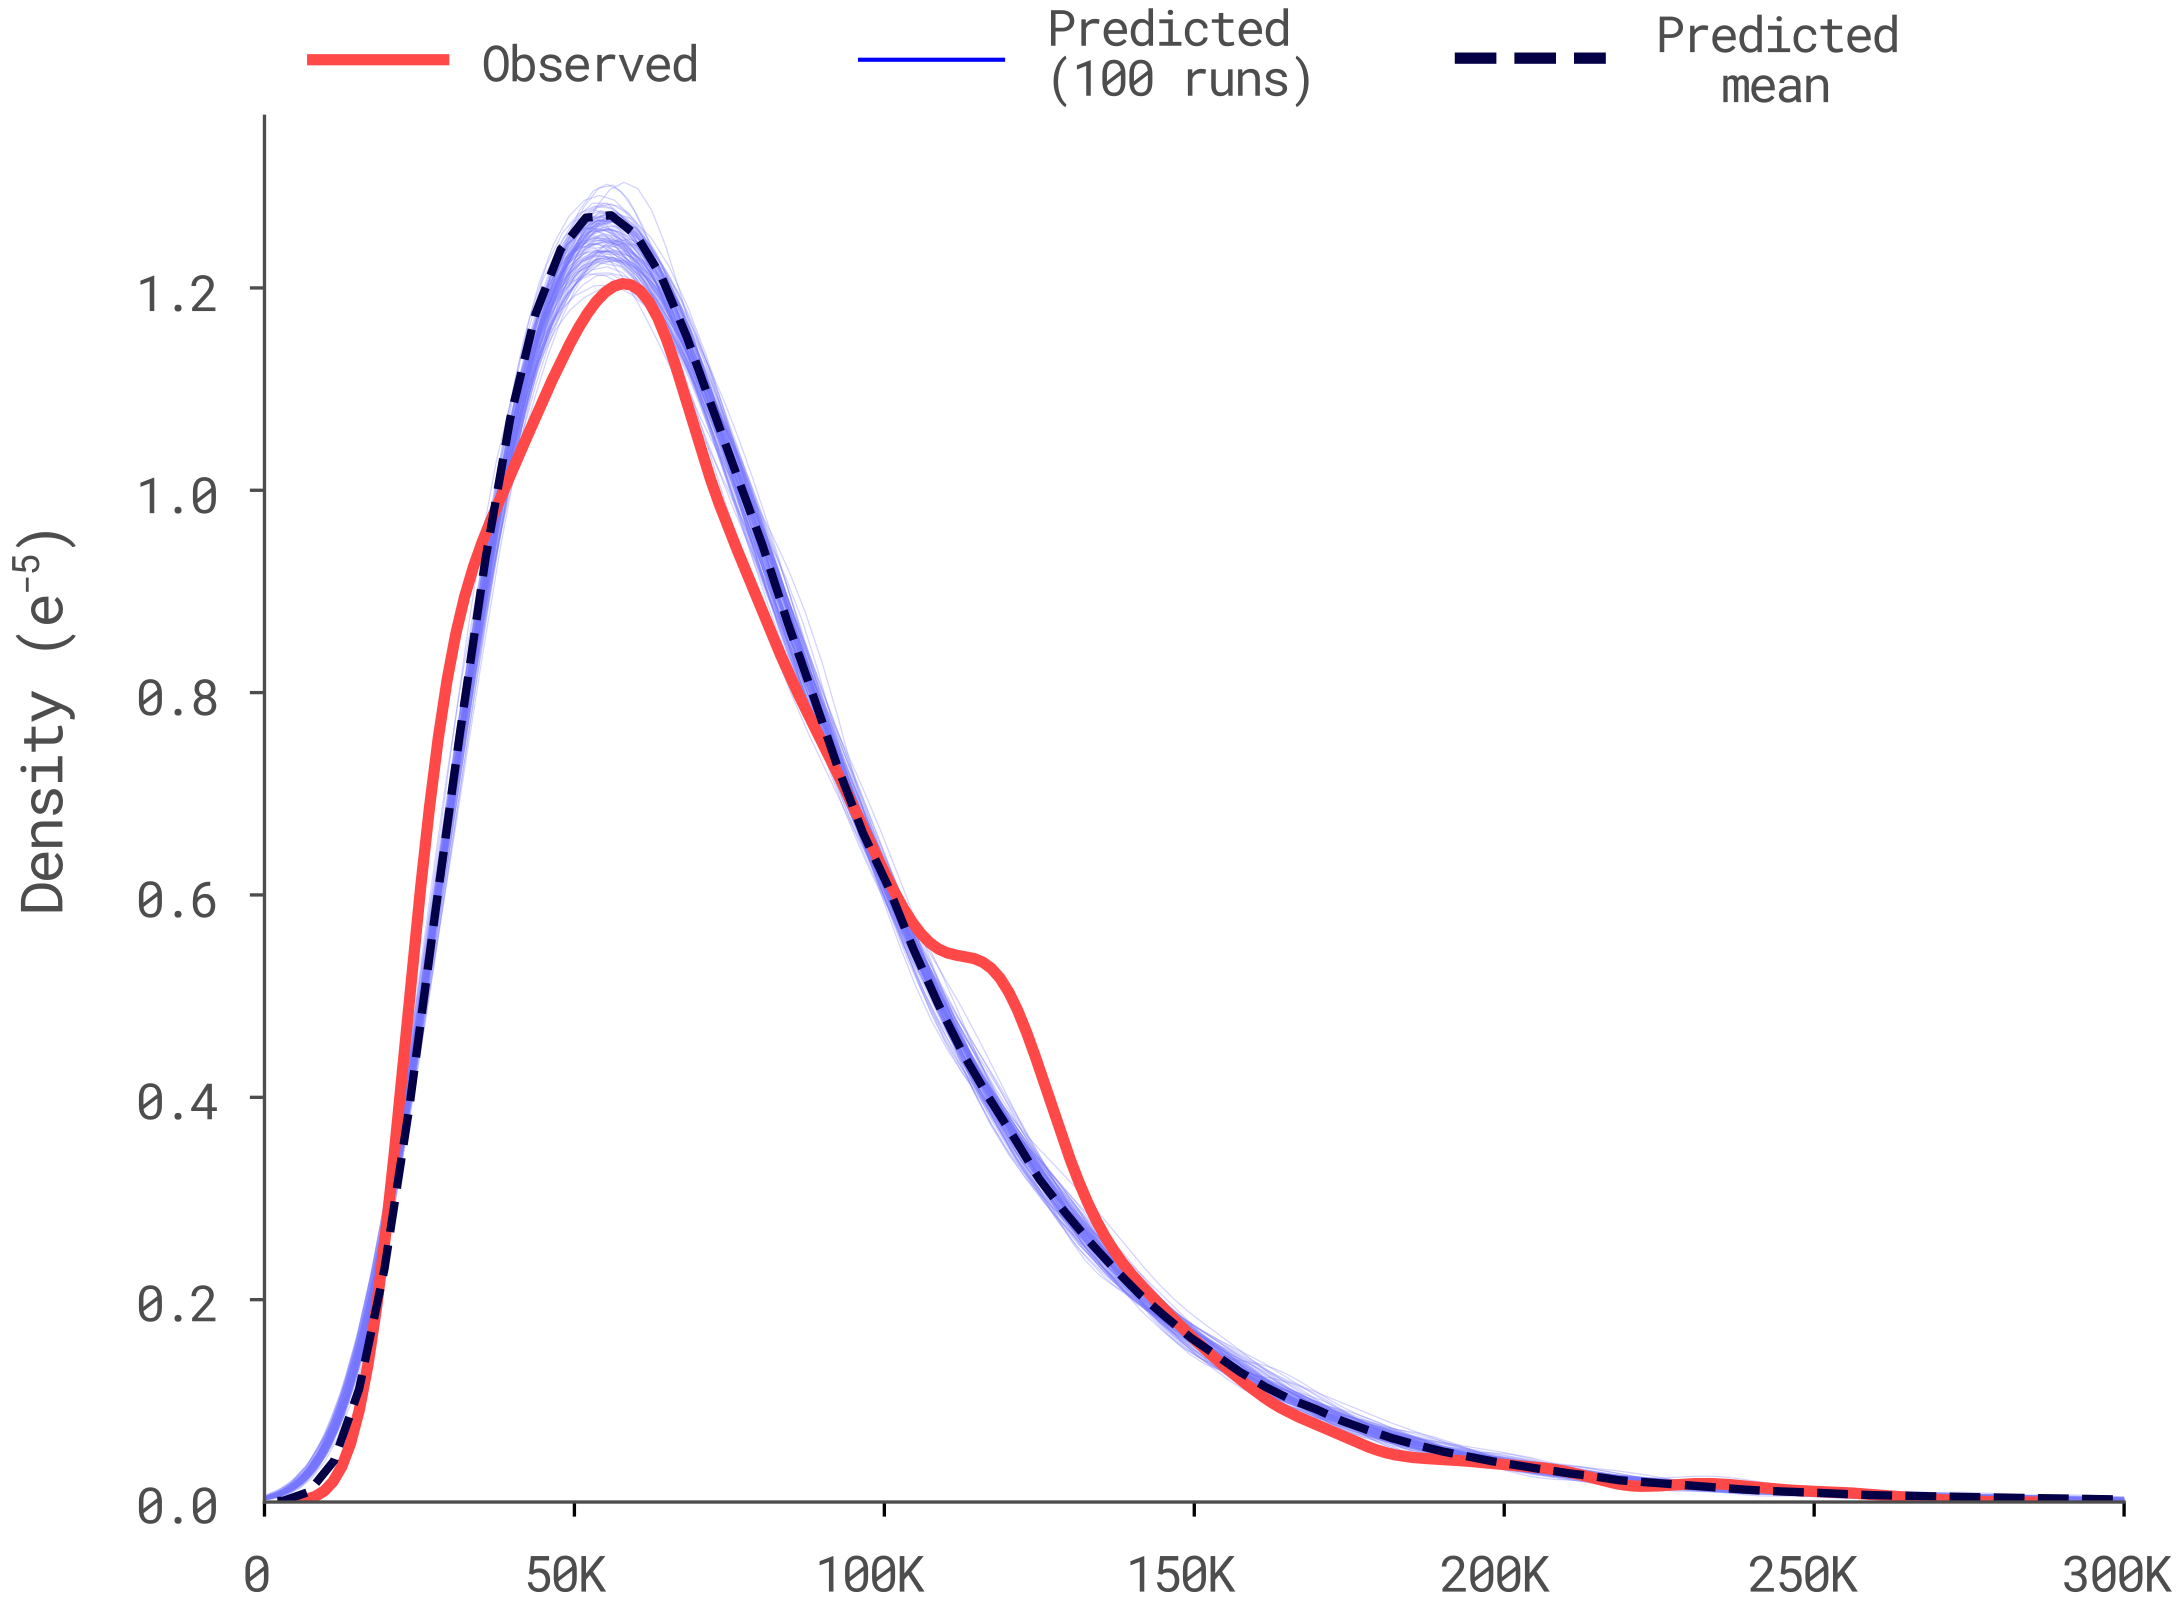
\includegraphics[width=0.7\textwidth]{images/ch5_agg_level/salary.png}
    \caption{Observed and predicted salary distribution for all individuals in the validation set}
    \setlength{\abovecaptionskip}{-10pt}
    \label{fig:validation_avg}
\end{figure}

\begin{landscape}
\begin{figure}[H]
    \centering
    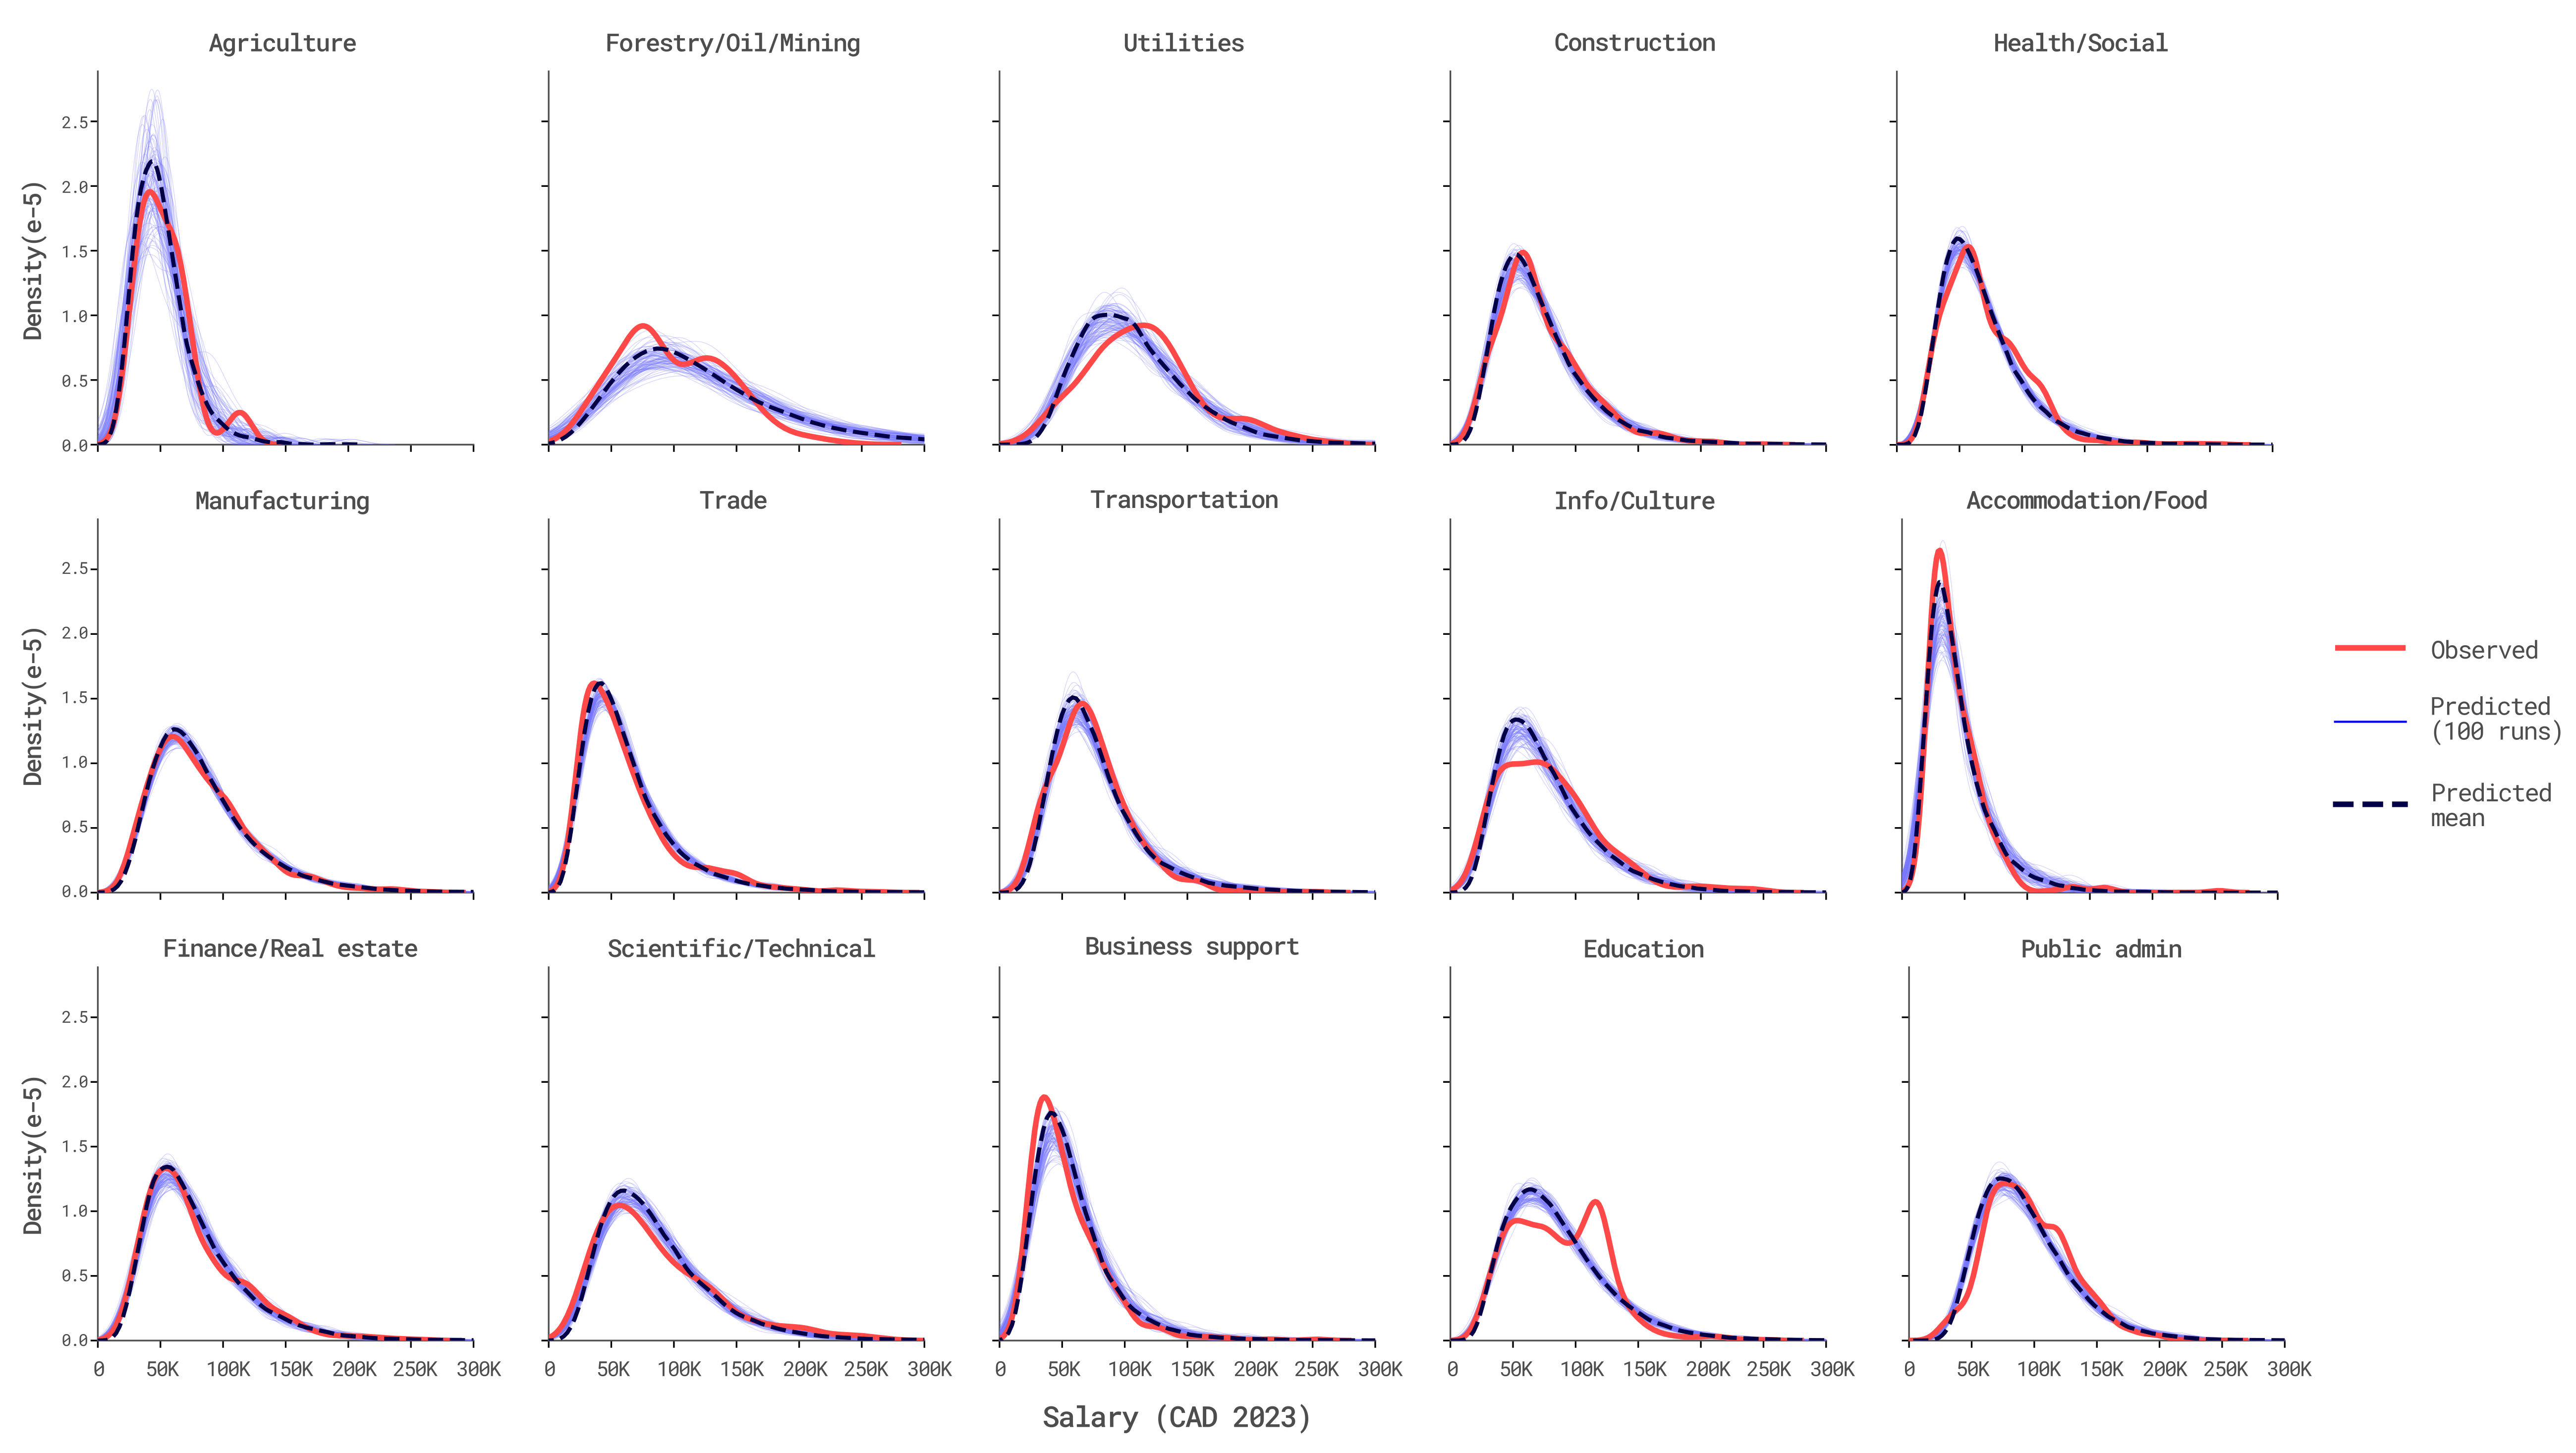
\includegraphics[width=1.3\textwidth]{images/ch5_agg_level/salary_ind.png}
    \caption{Observed and predicted salary distribution by Industry}
    \setlength{\abovecaptionskip}{-30pt}
    \label{fig:validation_industry}
\end{figure}


\begin{figure}[H]
    \centering
    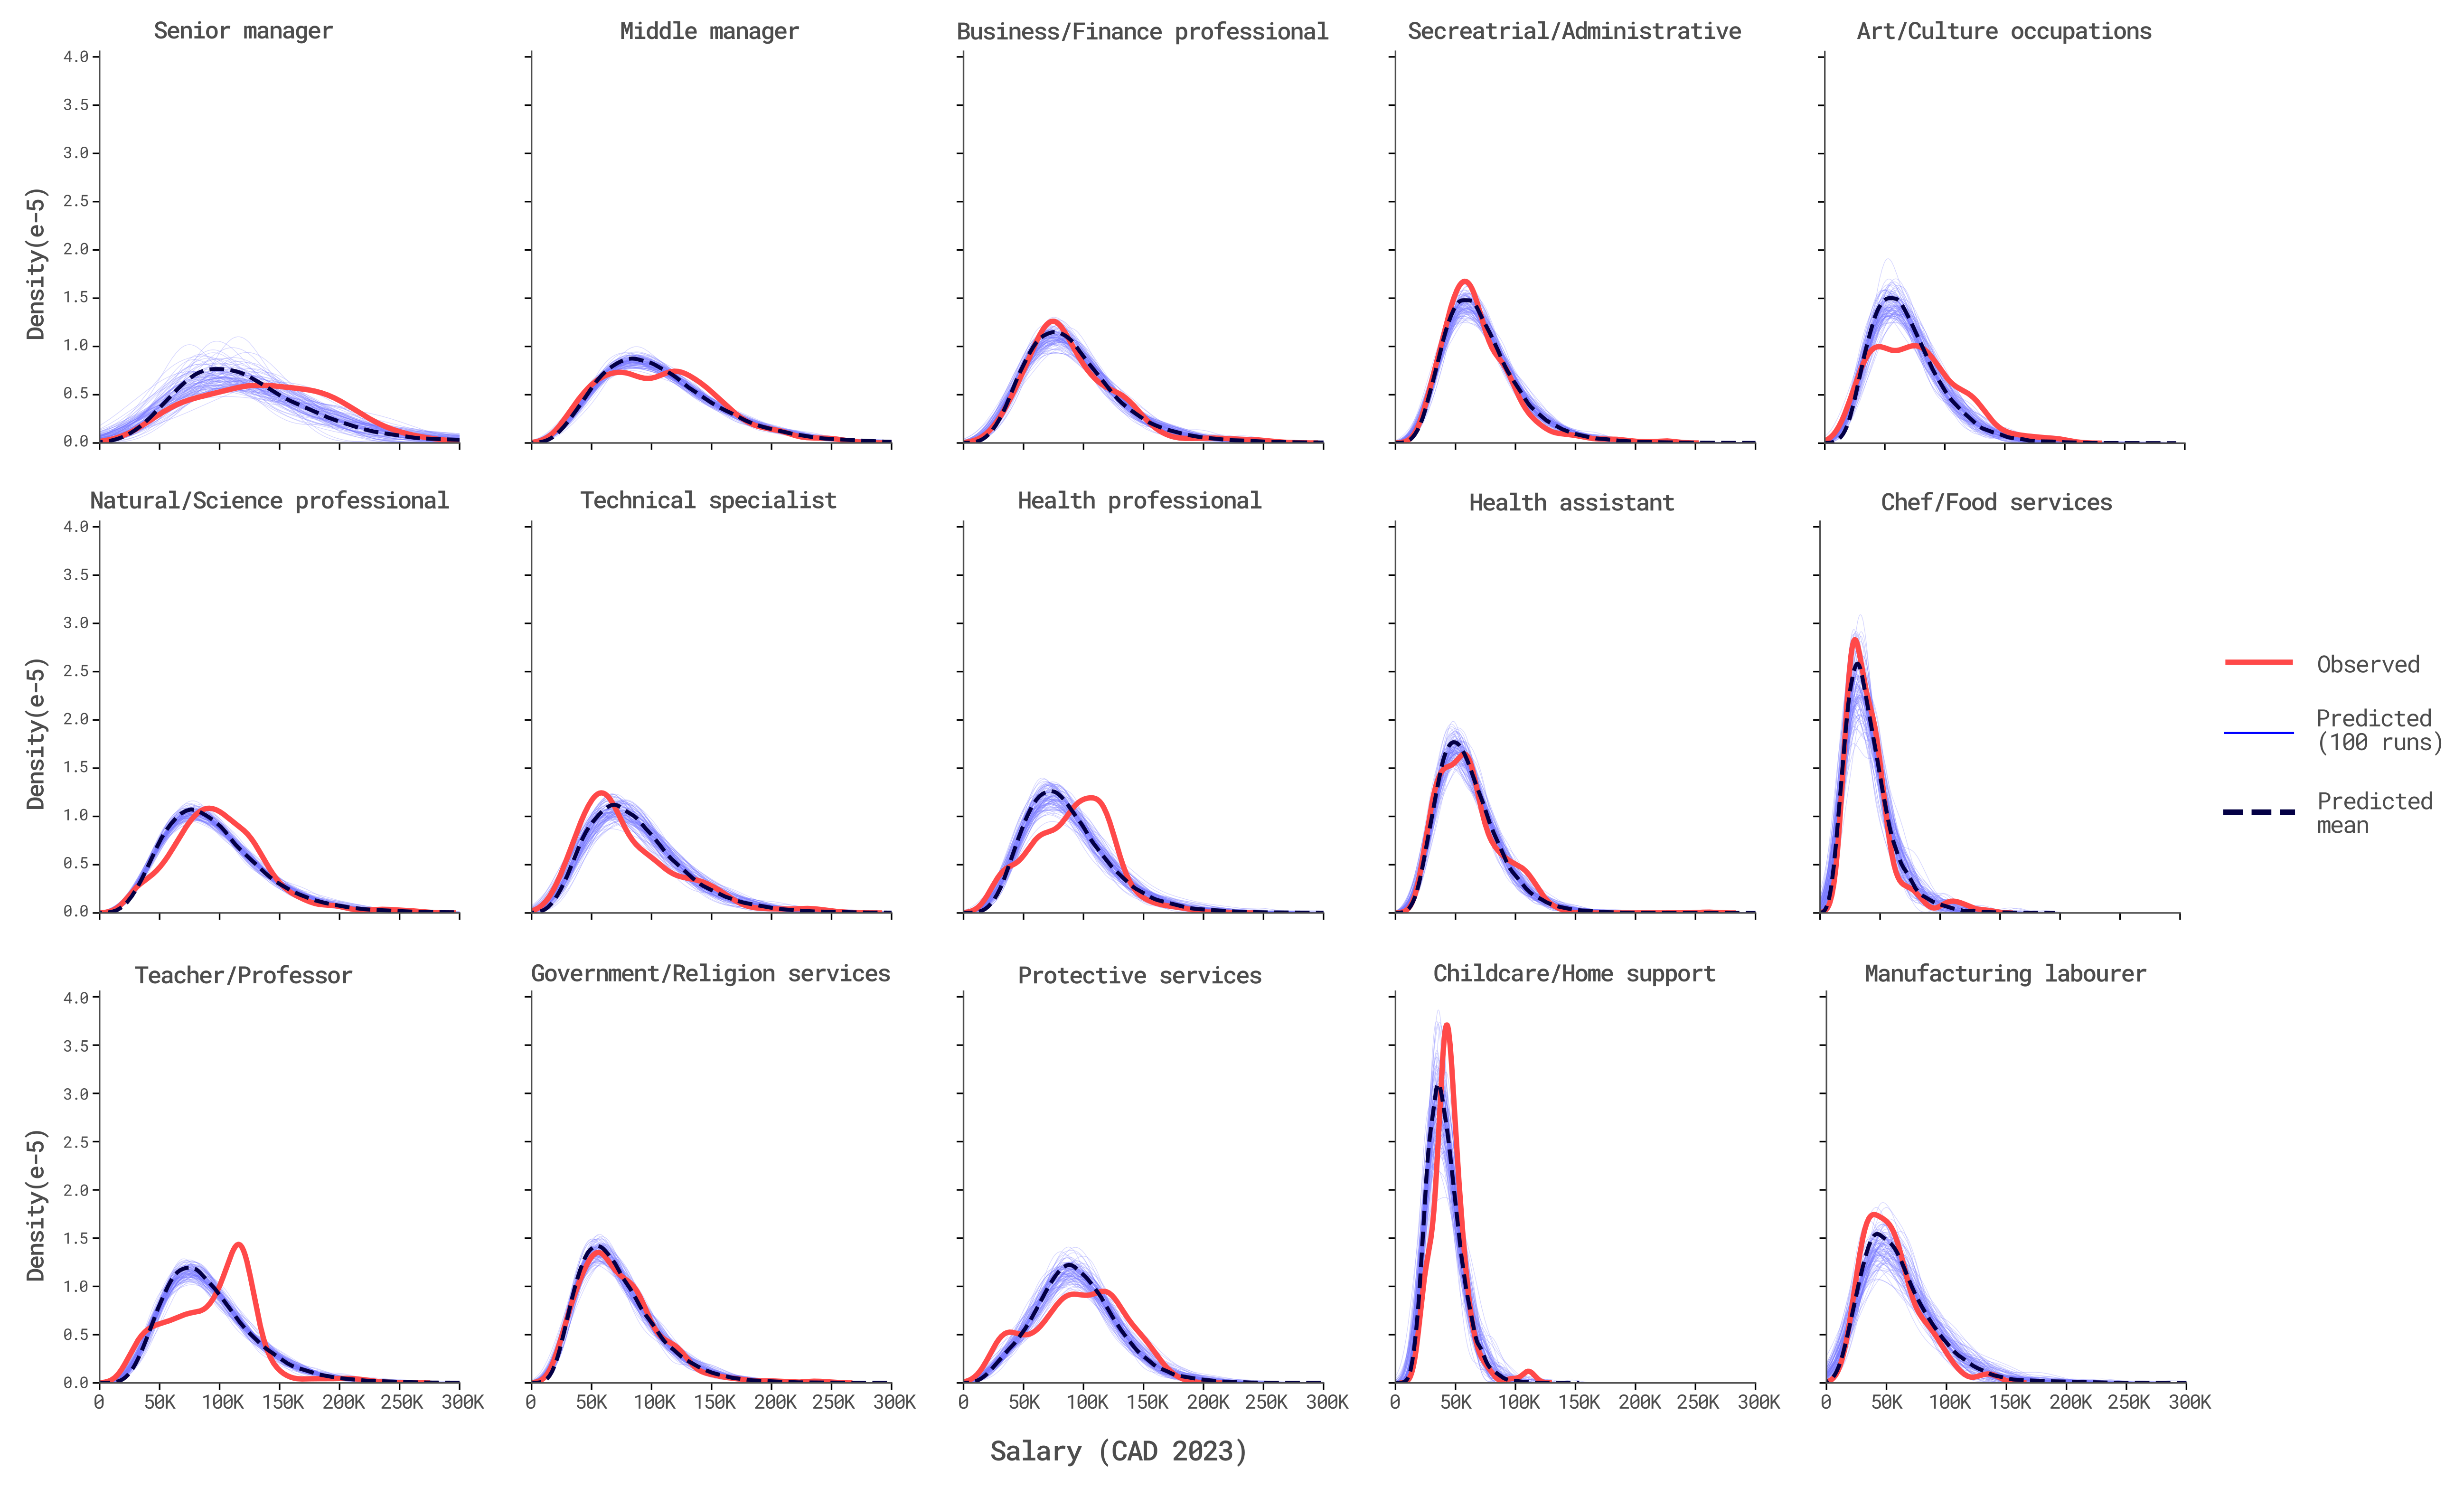
\includegraphics[width=1.3\textwidth]{images/ch5_agg_level/salary_occ.png}
    \caption{Observed and predicted salary distribution by Occupation}
    \setlength{\abovecaptionskip}{-15pt}
    \label{fig:validation_occupation}
\end{figure}
\end{landscape}

\subsection{Disaggregated level }

For the disaggregated level, \Cref{fig:validation_disagg} compares the following elements for a random set of workers. 

\begin{itemize}
    \item The observed salary: salary reported by the worker in the SLID. 

    \item The predicted salary: the expected value of the posterior salary distribution using the final model. 
    
    \item The posterior salary distribution is the estimated salary distribution for that worker given their attributes.
    
    \item The posterior salary distribution of similar workers: This is the reference case to compare with the previous distribution (posterior salary distribution) and represents the average salary distribution of workers with the same attributes (variables used in the model estimation). This distribution also allows us to identify whether the observed salary is an outlier compared to workers with the same characteristics. 
\end{itemize}

The comparison between these four elements provides a detailed perspective of the model's ability to represent data at the disaggregated level. The comparison between the observed salary and the posterior salary distribution of similar workers illustrates the stochastic nature of salaries. Given the size of the validation dataset, it is unfeasible to report this chart for all workers. However, the GitHub repository of this thesis provides a Jupyter notebook that allows to explore and create this chart for any worker in the dataset. 

\begin{landscape}
    \begin{figure}[H]
        \centering
        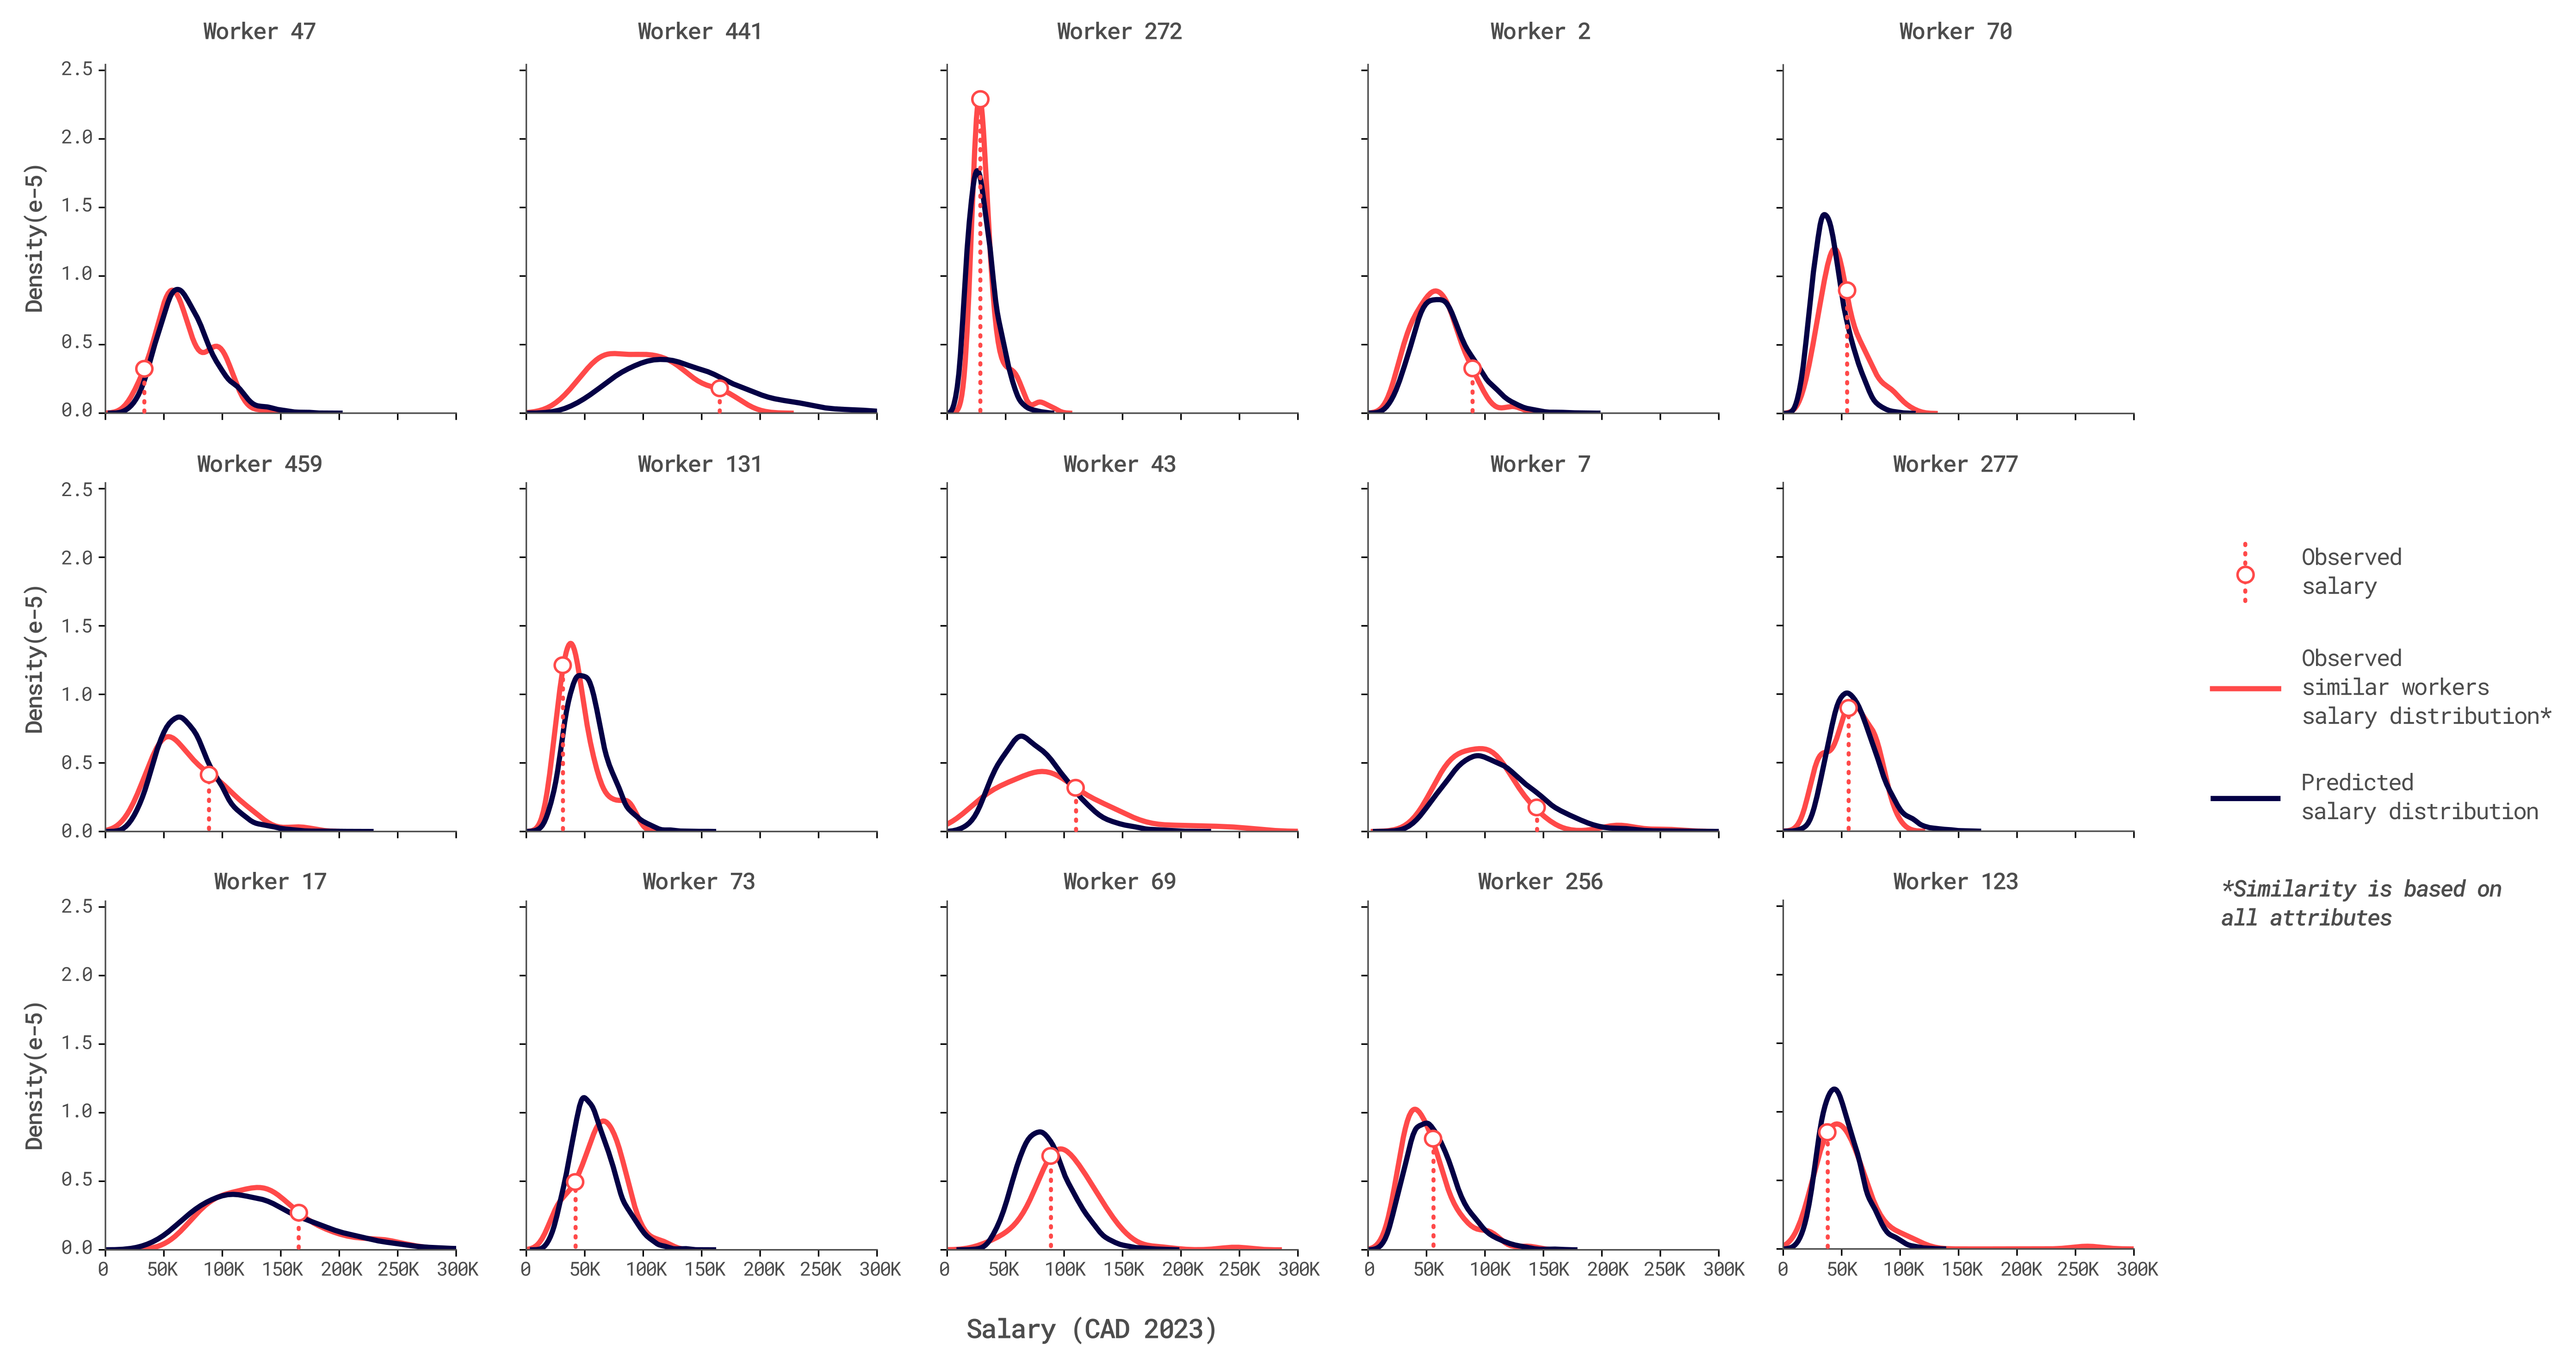
\includegraphics[width=1.3\textwidth]{images/ch5_disagg_level/workers.png}
        \caption{Disaggregated analysis of salary distribution for 15 random selected workers within the validation dataset}
        \setlength{\abovecaptionskip}{-10pt}
        \label{fig:validation_disagg}
    \end{figure}
\end{landscape}




% Set graphics path
\graphicspath{{images/ch6_class_person/}}
\chapter{Model integration}

\section{Integration with the existing implementation}

\section{Model comparison: proposed vs. existent}
% Insert image from tex file
% \input{images/test4}

% Insert image from svg file
\begin{figure}[h]
    \centering
    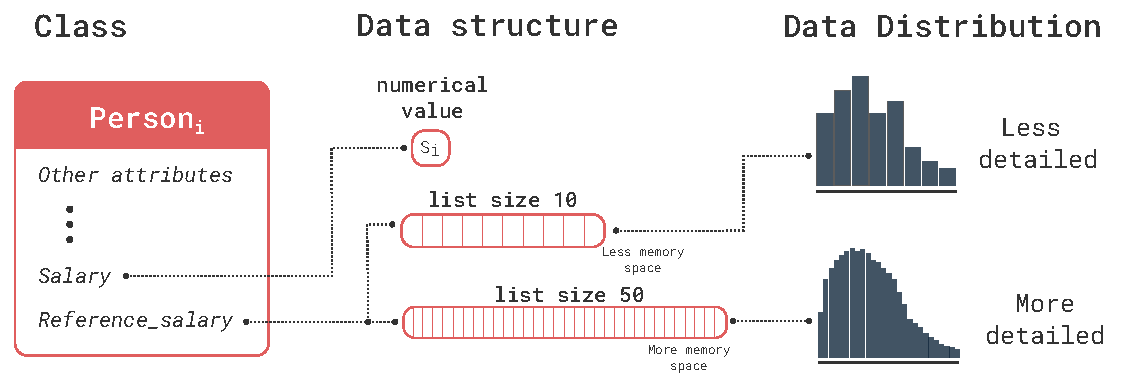
\includegraphics[width=16cm]{class_person.pdf}
    \caption{Representation of salary within the existent framework.}
    \label{fig:class_person}
\end{figure}



\chapter{Conclusions}

The hierarchical structure in labour markets defines many attributes of both the firms and the individuals. According to the findings in this thesis, this structure is closely related with the observed wage differentials. Therefore, the inclusion of this structure in the modelling process will improve significantly the results and accuracy of the model. However, this structure also needs to consider the relationships between the different levels. The hierarchical or multilevel model is an approach that meets these requirements because it represents the hierarchical structure while also models the complex relationships between the multiple levels by sharing information between them. 

Given the stochastic nature of simulations, the use of a random component seems to be more flexible and realistic than the use of point estimates to represent salaries within the labour market. As salaries are positive a right skewed, the application of the regular linear regression model could be misrepresenting the random component of salary definition. As suggested by the literature, the use of the Gamma distribution in conjunction with a systematic component improves the model performance and allows to capture the particularities of the observed salaries. 

Besides the model structure, the application of the Bayesian inference framework allows to extract more information from the data by producing probability distributions instead of point estimates. This is more evident when modelling out-of-sample salary distributions at both the aggregated and disaggregated level with high accuracy and a good bias-variance balance, which demonstrates its potential to produce robust estimations. However, these advantages come with a cost in terms of computational power. 

\section{Future work}

Based on the results presented in Chapter 5 and Chapter 6, the proposed model needs to be tested within the Harmon's AMB implementation of the labour market in ILUTE. Although Chapter 6 compares the methodologies of the existent and proposed model, applying the last one in a simulation setting will provide evidence whether the use of salary probability distributions outperforms the use of point estimates. 

As the hierarchical model is also applicable to spatial problems, the proposed model could benefit from including job location as a predictor at the industry level. This approach will improve the representation of the decision-making process within the job matching process in ILUTE and provide a more realistic. 

The proposed model is not considering any variation between the model's parameters. However, a possible way to improve the predictive accuracy could be to model the covariance between the predictors by setting a prior over the correlation matrix using the LJK distribution. This distribution provides a way to define a uniform distribution of all possible positive defined correlation matrices. With this approach, some labour market distributions such as the gender and level of education can be better represented for some specific industries and occupations. 

On the other hand, although the SLID dataset is a detailed data source, future efforts should be focused on using more updated datasets to validate the effects of recent changes in the labour force in the estimated models. In this matter, Statistics Canada has an interesting set of statistical programs but most of them require an application process to access this data. Under the light of new data, the proposed model is expected to benefit from the online learning scheme, in which the model can be easily updated under the Bayesian framework. This update just consider that the results of this thesis are the priors to be updated using the new data. 

Another important aspect to consider when evaluating the possible effects of current and future changes in the labour market is the increment of salaries over time. Given the stability observed in most of the salaries during the period of study, the autoregressive nature of the time series could be obviated. However, as the labour markets are continuously changing this behaviour can be different in the future. Therefore, this is something to consider in future updates of this model. 
\include{chapters/8_future_work}

\bibliographystyle{apalike}
\bibliography{bibliography}

\appendix
\chapter{Posterior distributions}\label{app:posterior_dists}

\section{Posterior distributions for the pooled model}

\begin{figure}[H]
    \centering
    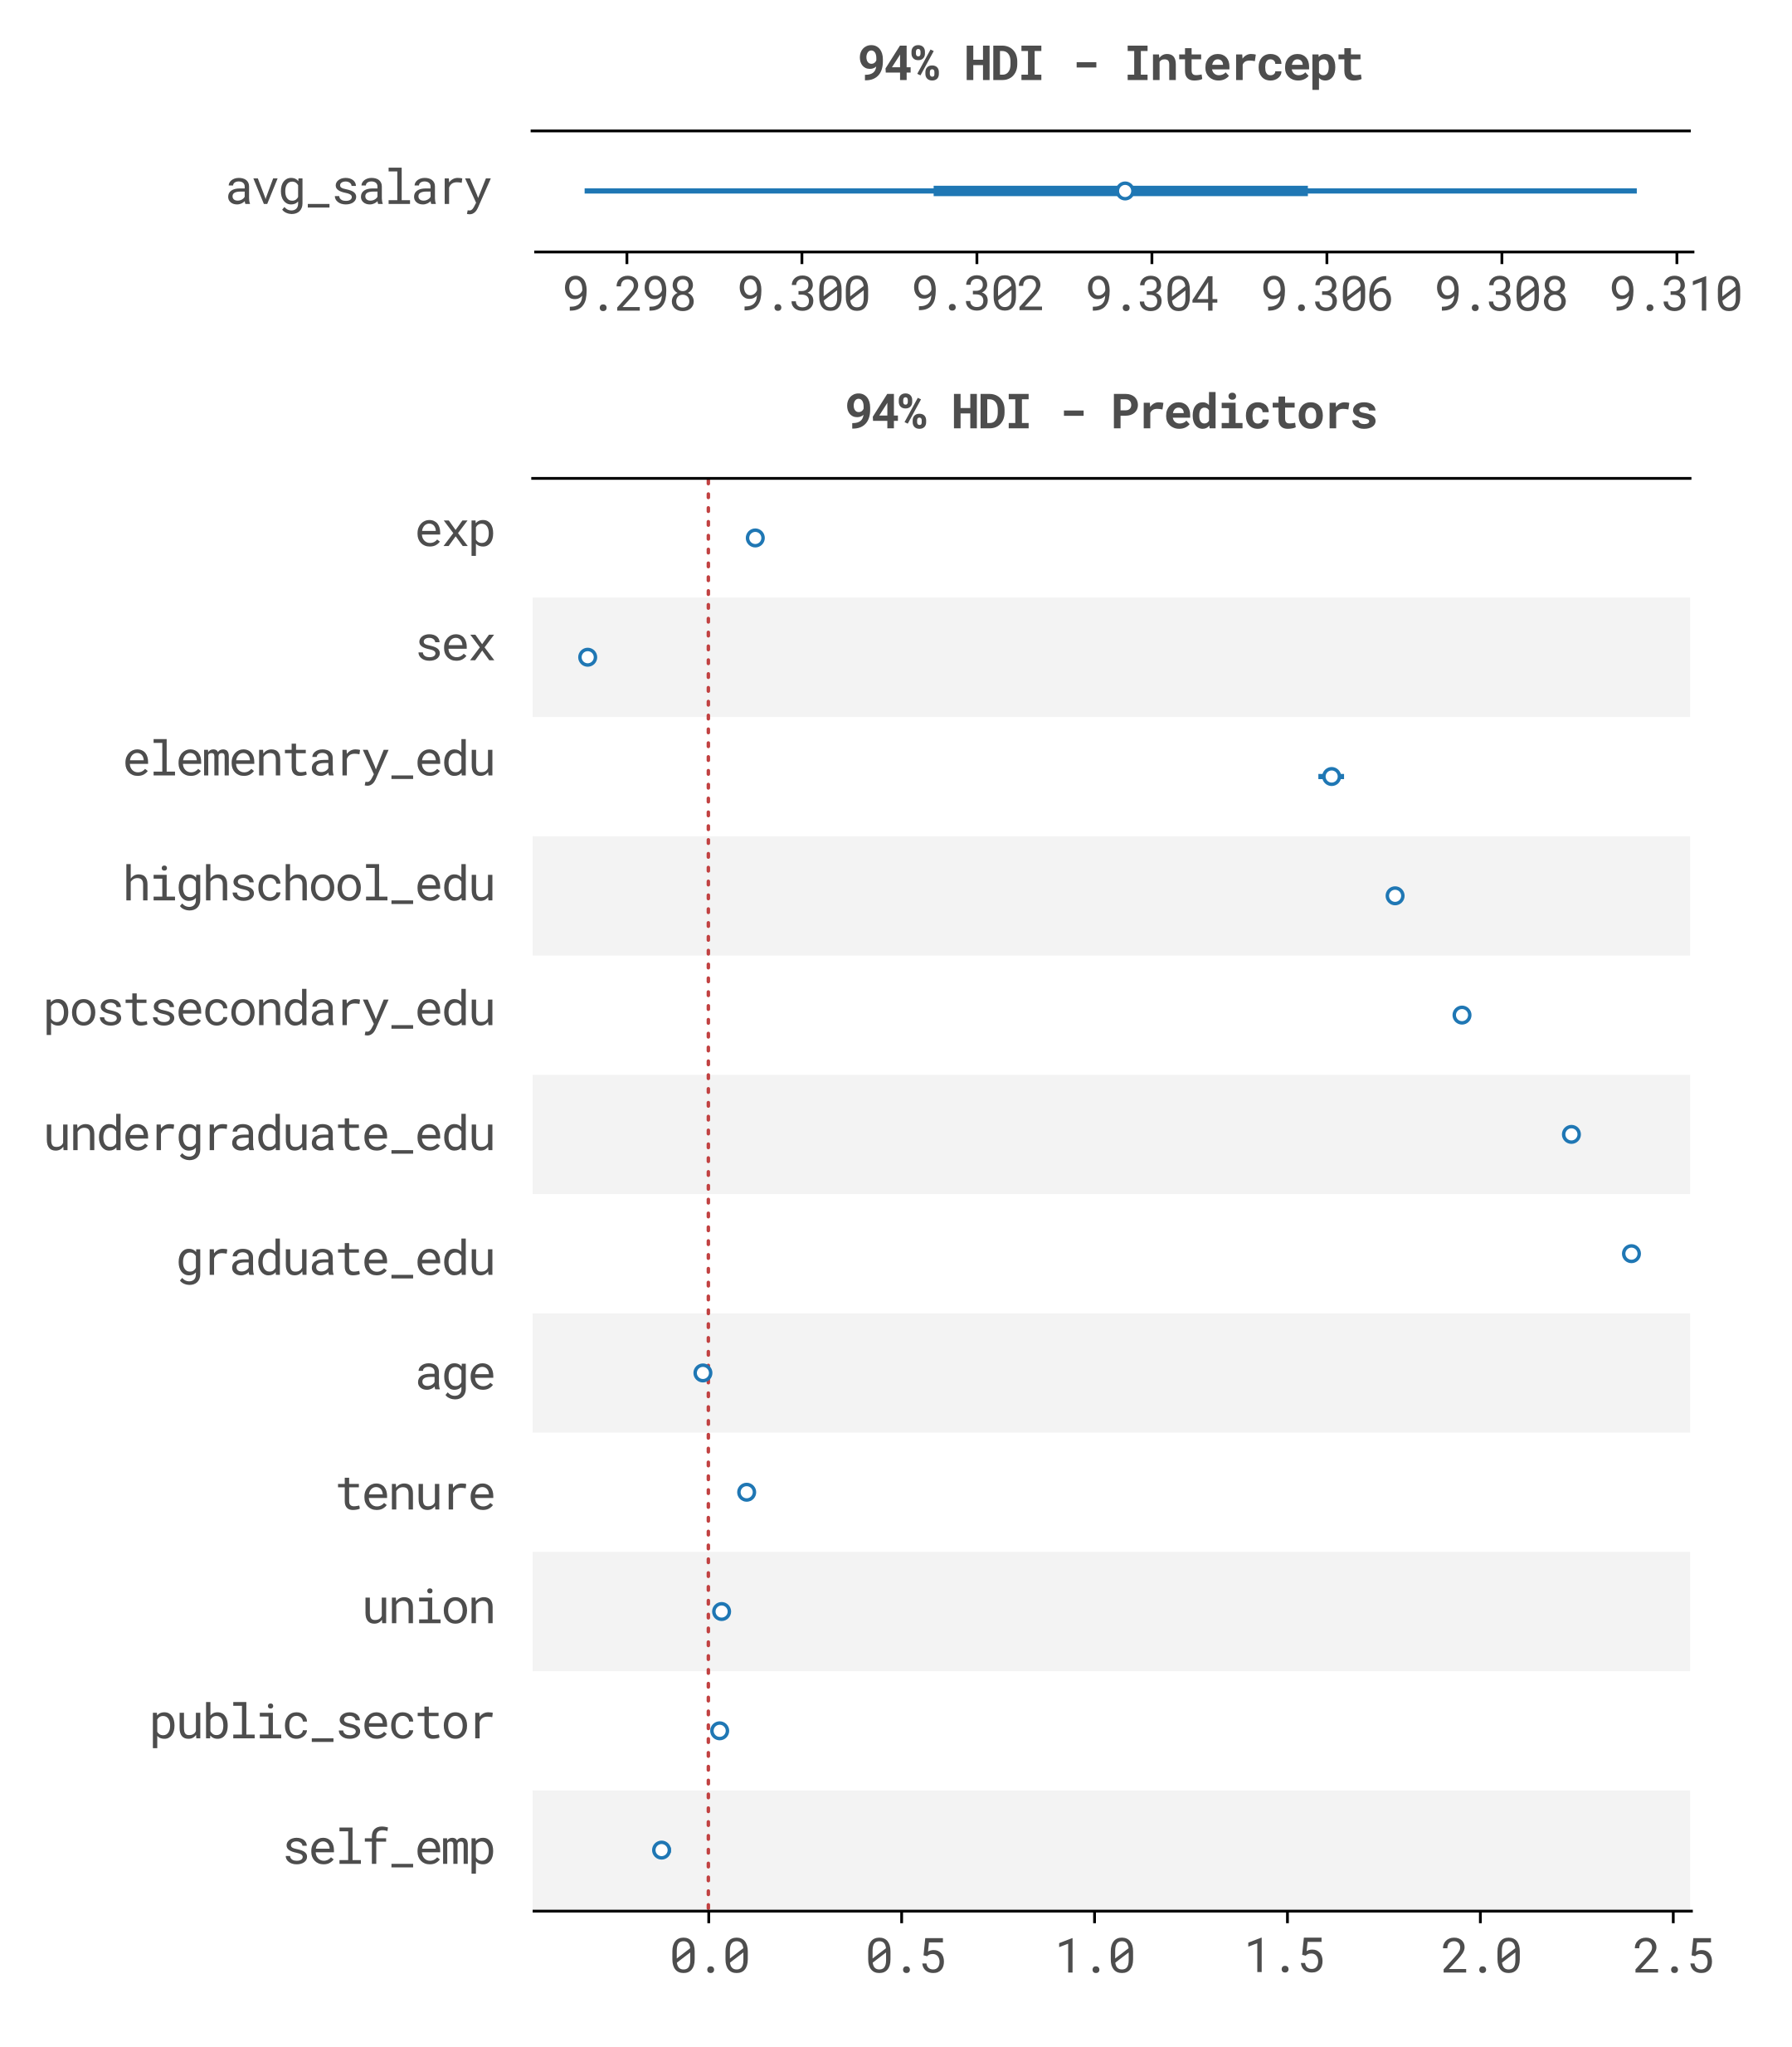
\includegraphics[width=0.6\textwidth]{images/appendix/pooled.png}
    \caption{Posterior distributions of model parameters for the pooled model.}
    \label{fig:posterior_dists_pooled}
\end{figure}

\section{Posterior distributions for the no-pooled model}

\begin{figure}[H]
    \centering
    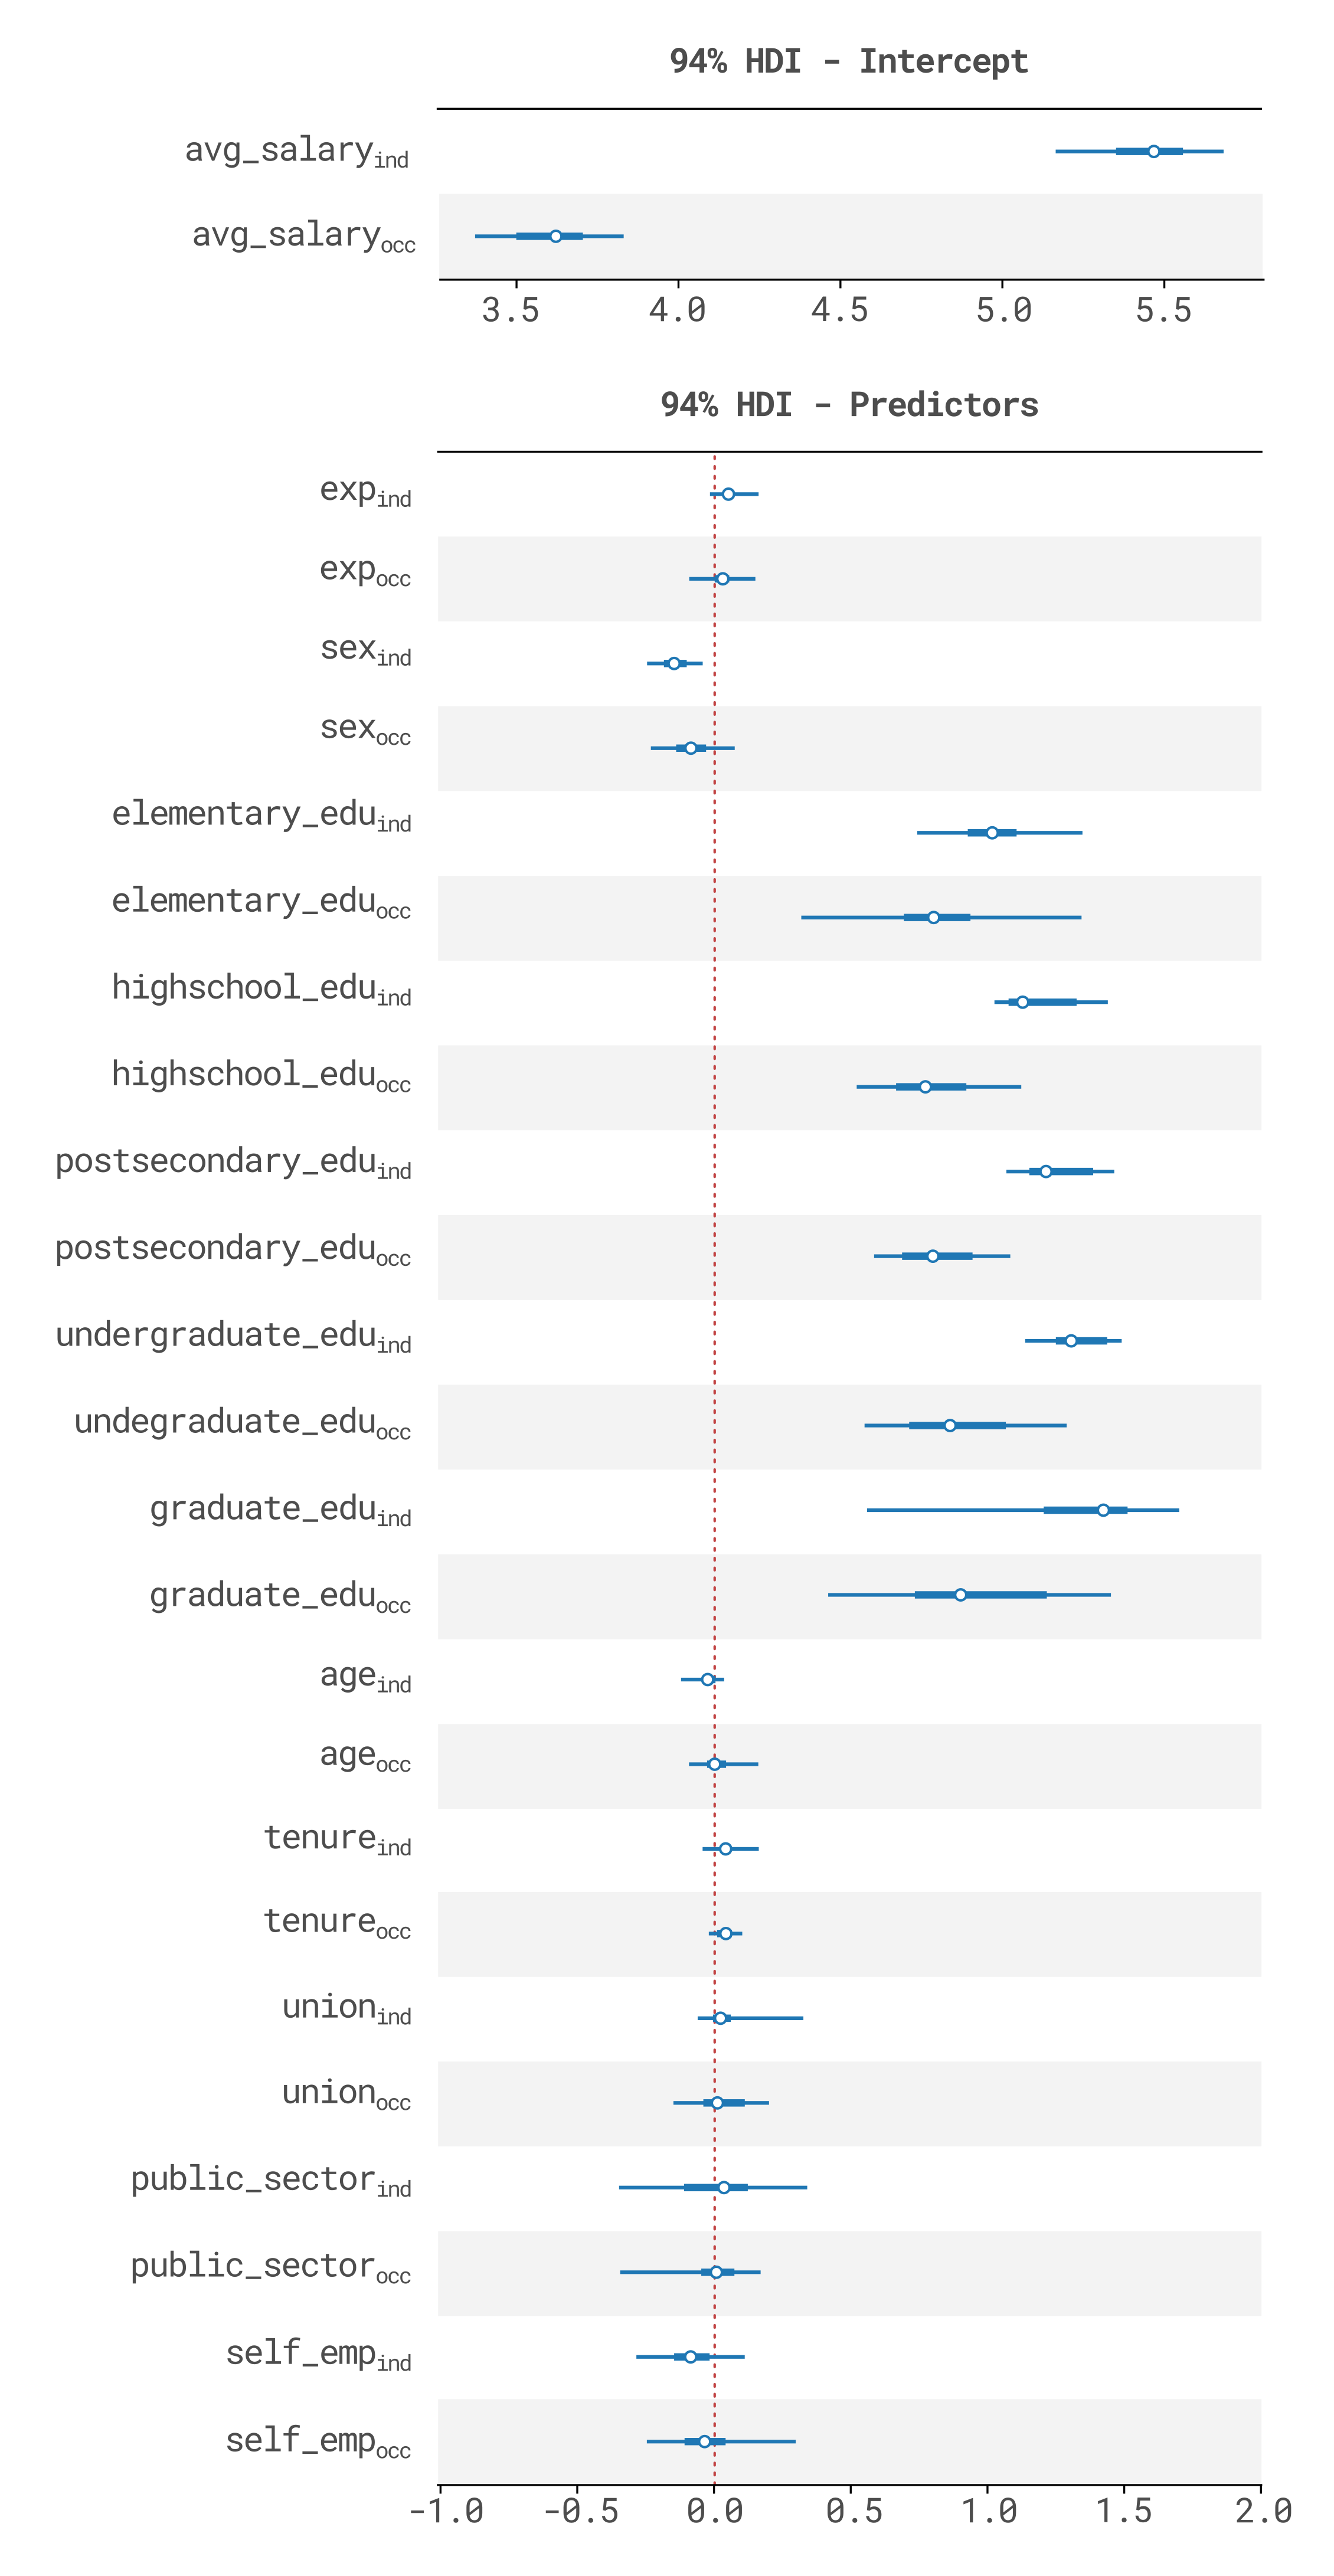
\includegraphics[width=0.6\textwidth]{images/appendix/no_pooled.png}
    \caption{Posterior distributions of model parameters for the no-pooled model (*All categories aggregated).}
    \label{fig:posterior_dists_nopooled}
\end{figure}

\section{Posterior distributions for the hierarchical model}

\begin{figure}[H]
    \centering
    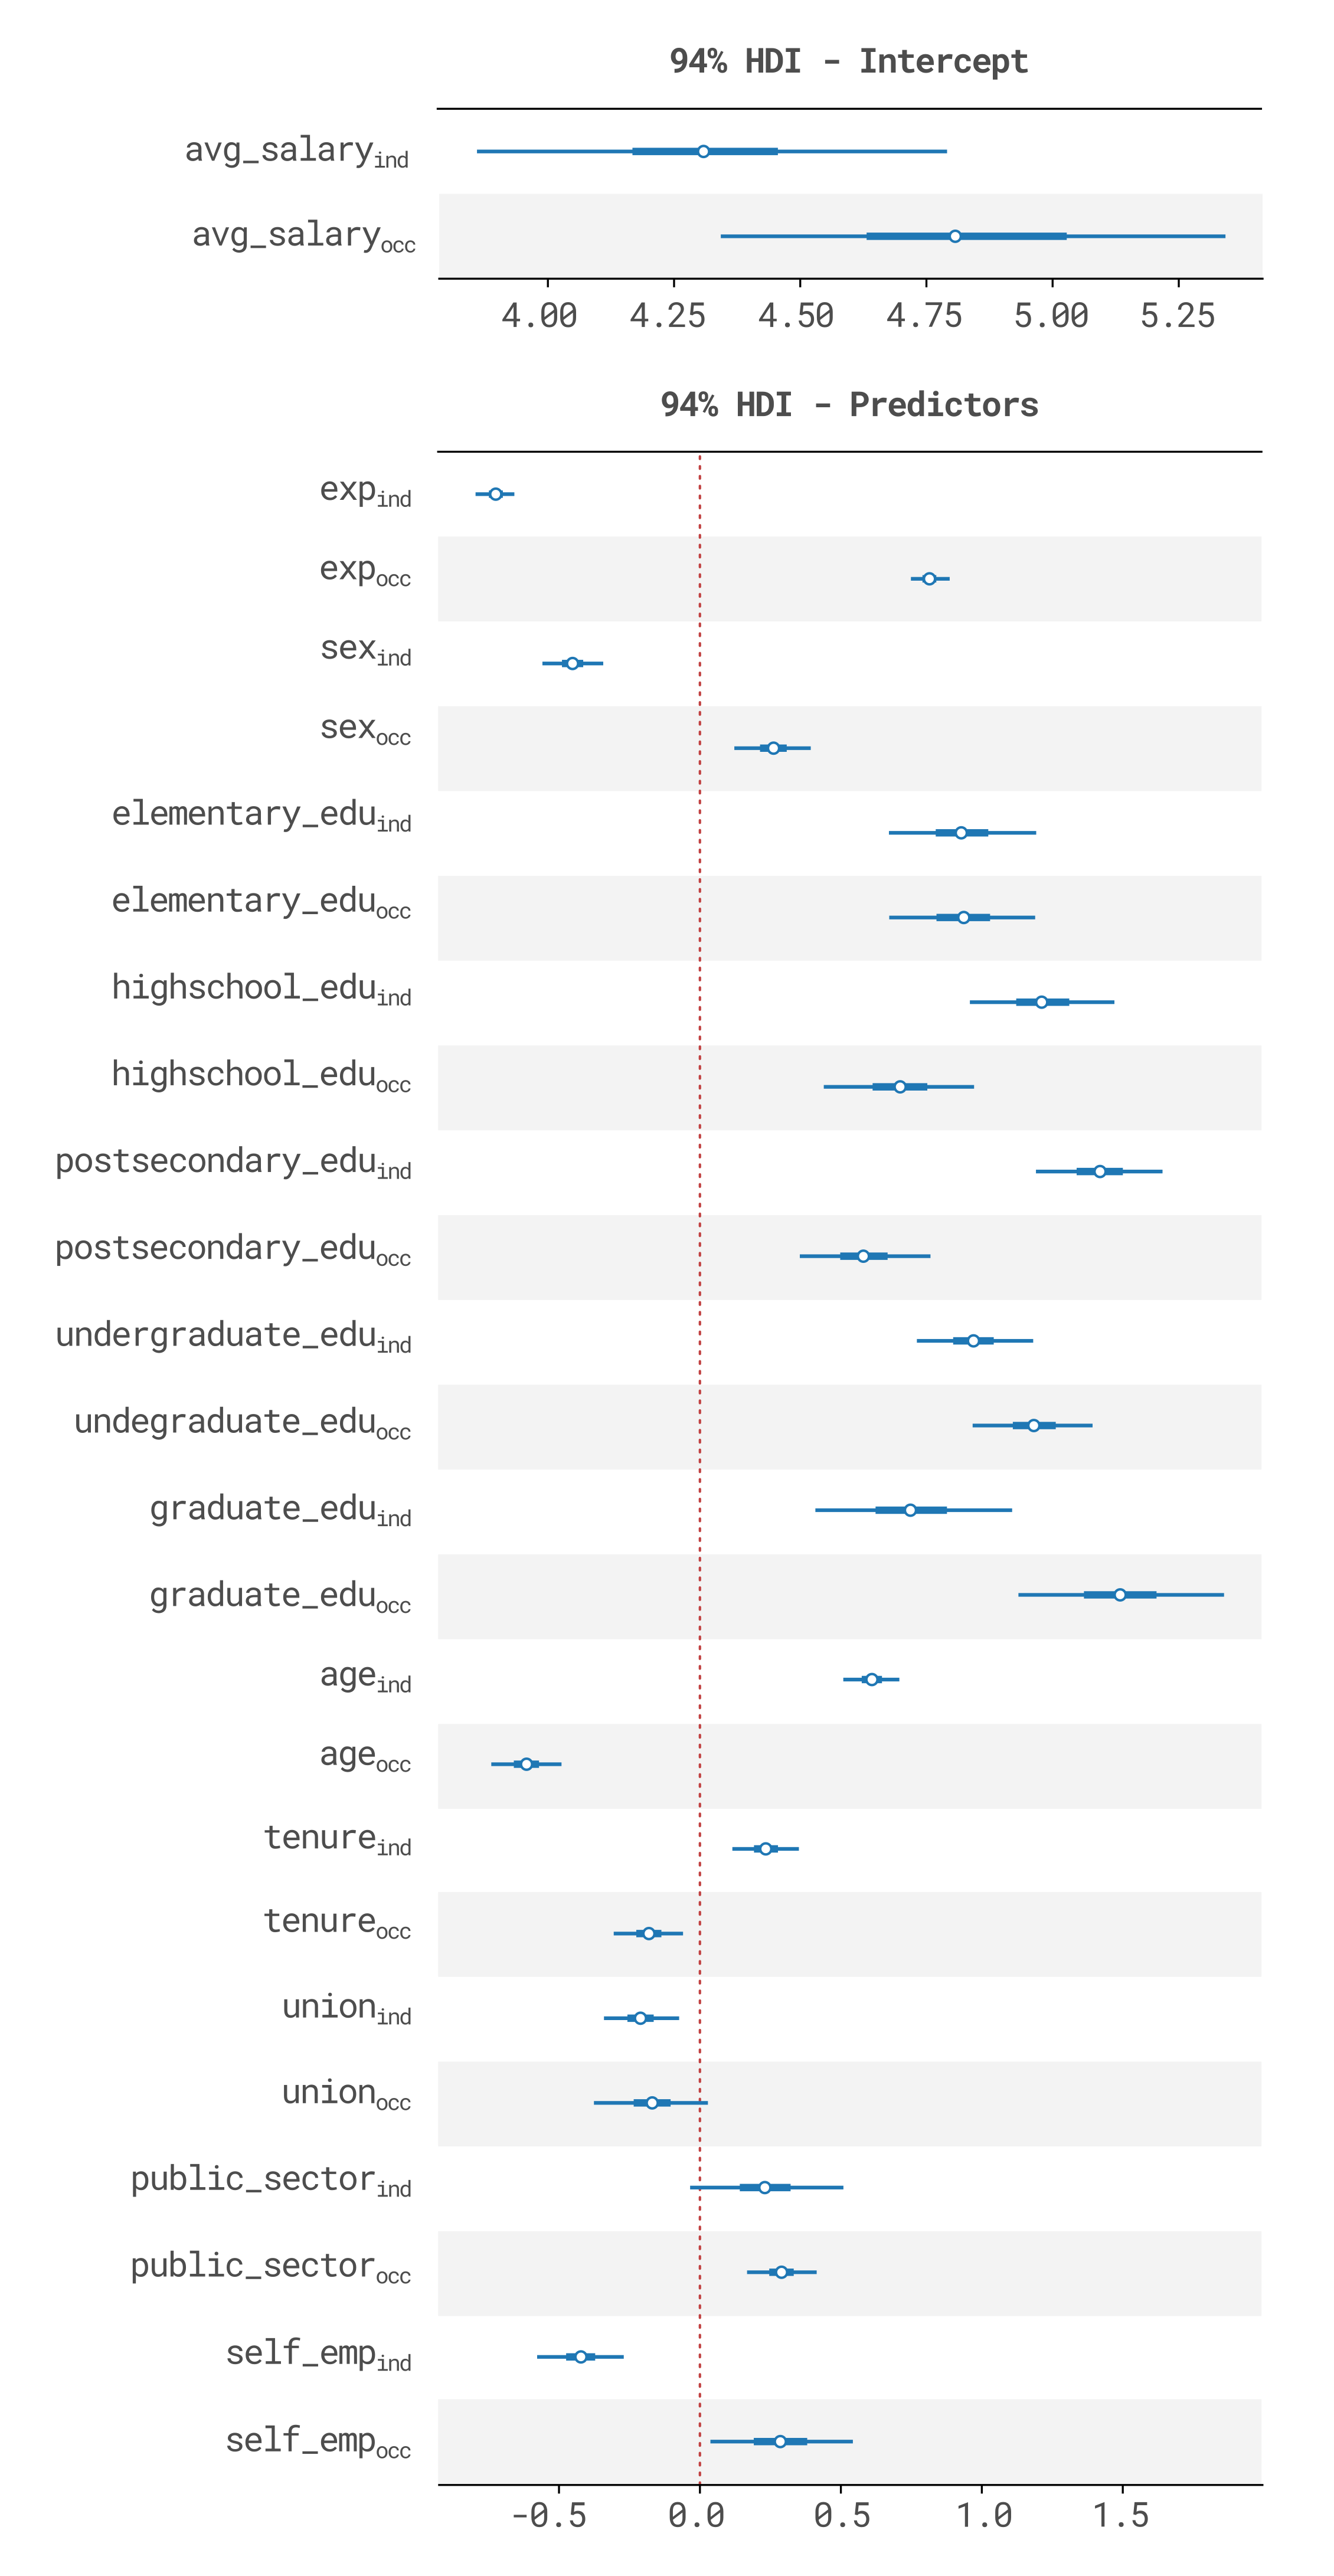
\includegraphics[width=0.6\textwidth]{images/appendix/hierarchical.png}
    \caption{Posterior distributions of model parameters for the hierarchical model (*All categories aggregated).}
    \label{fig:posterior_dists_hierarchical}
\end{figure}


\chapter{Posterior distributions for final model}\label{app:posterior_dists_final}

\begin{figure}[H]
    \centering
    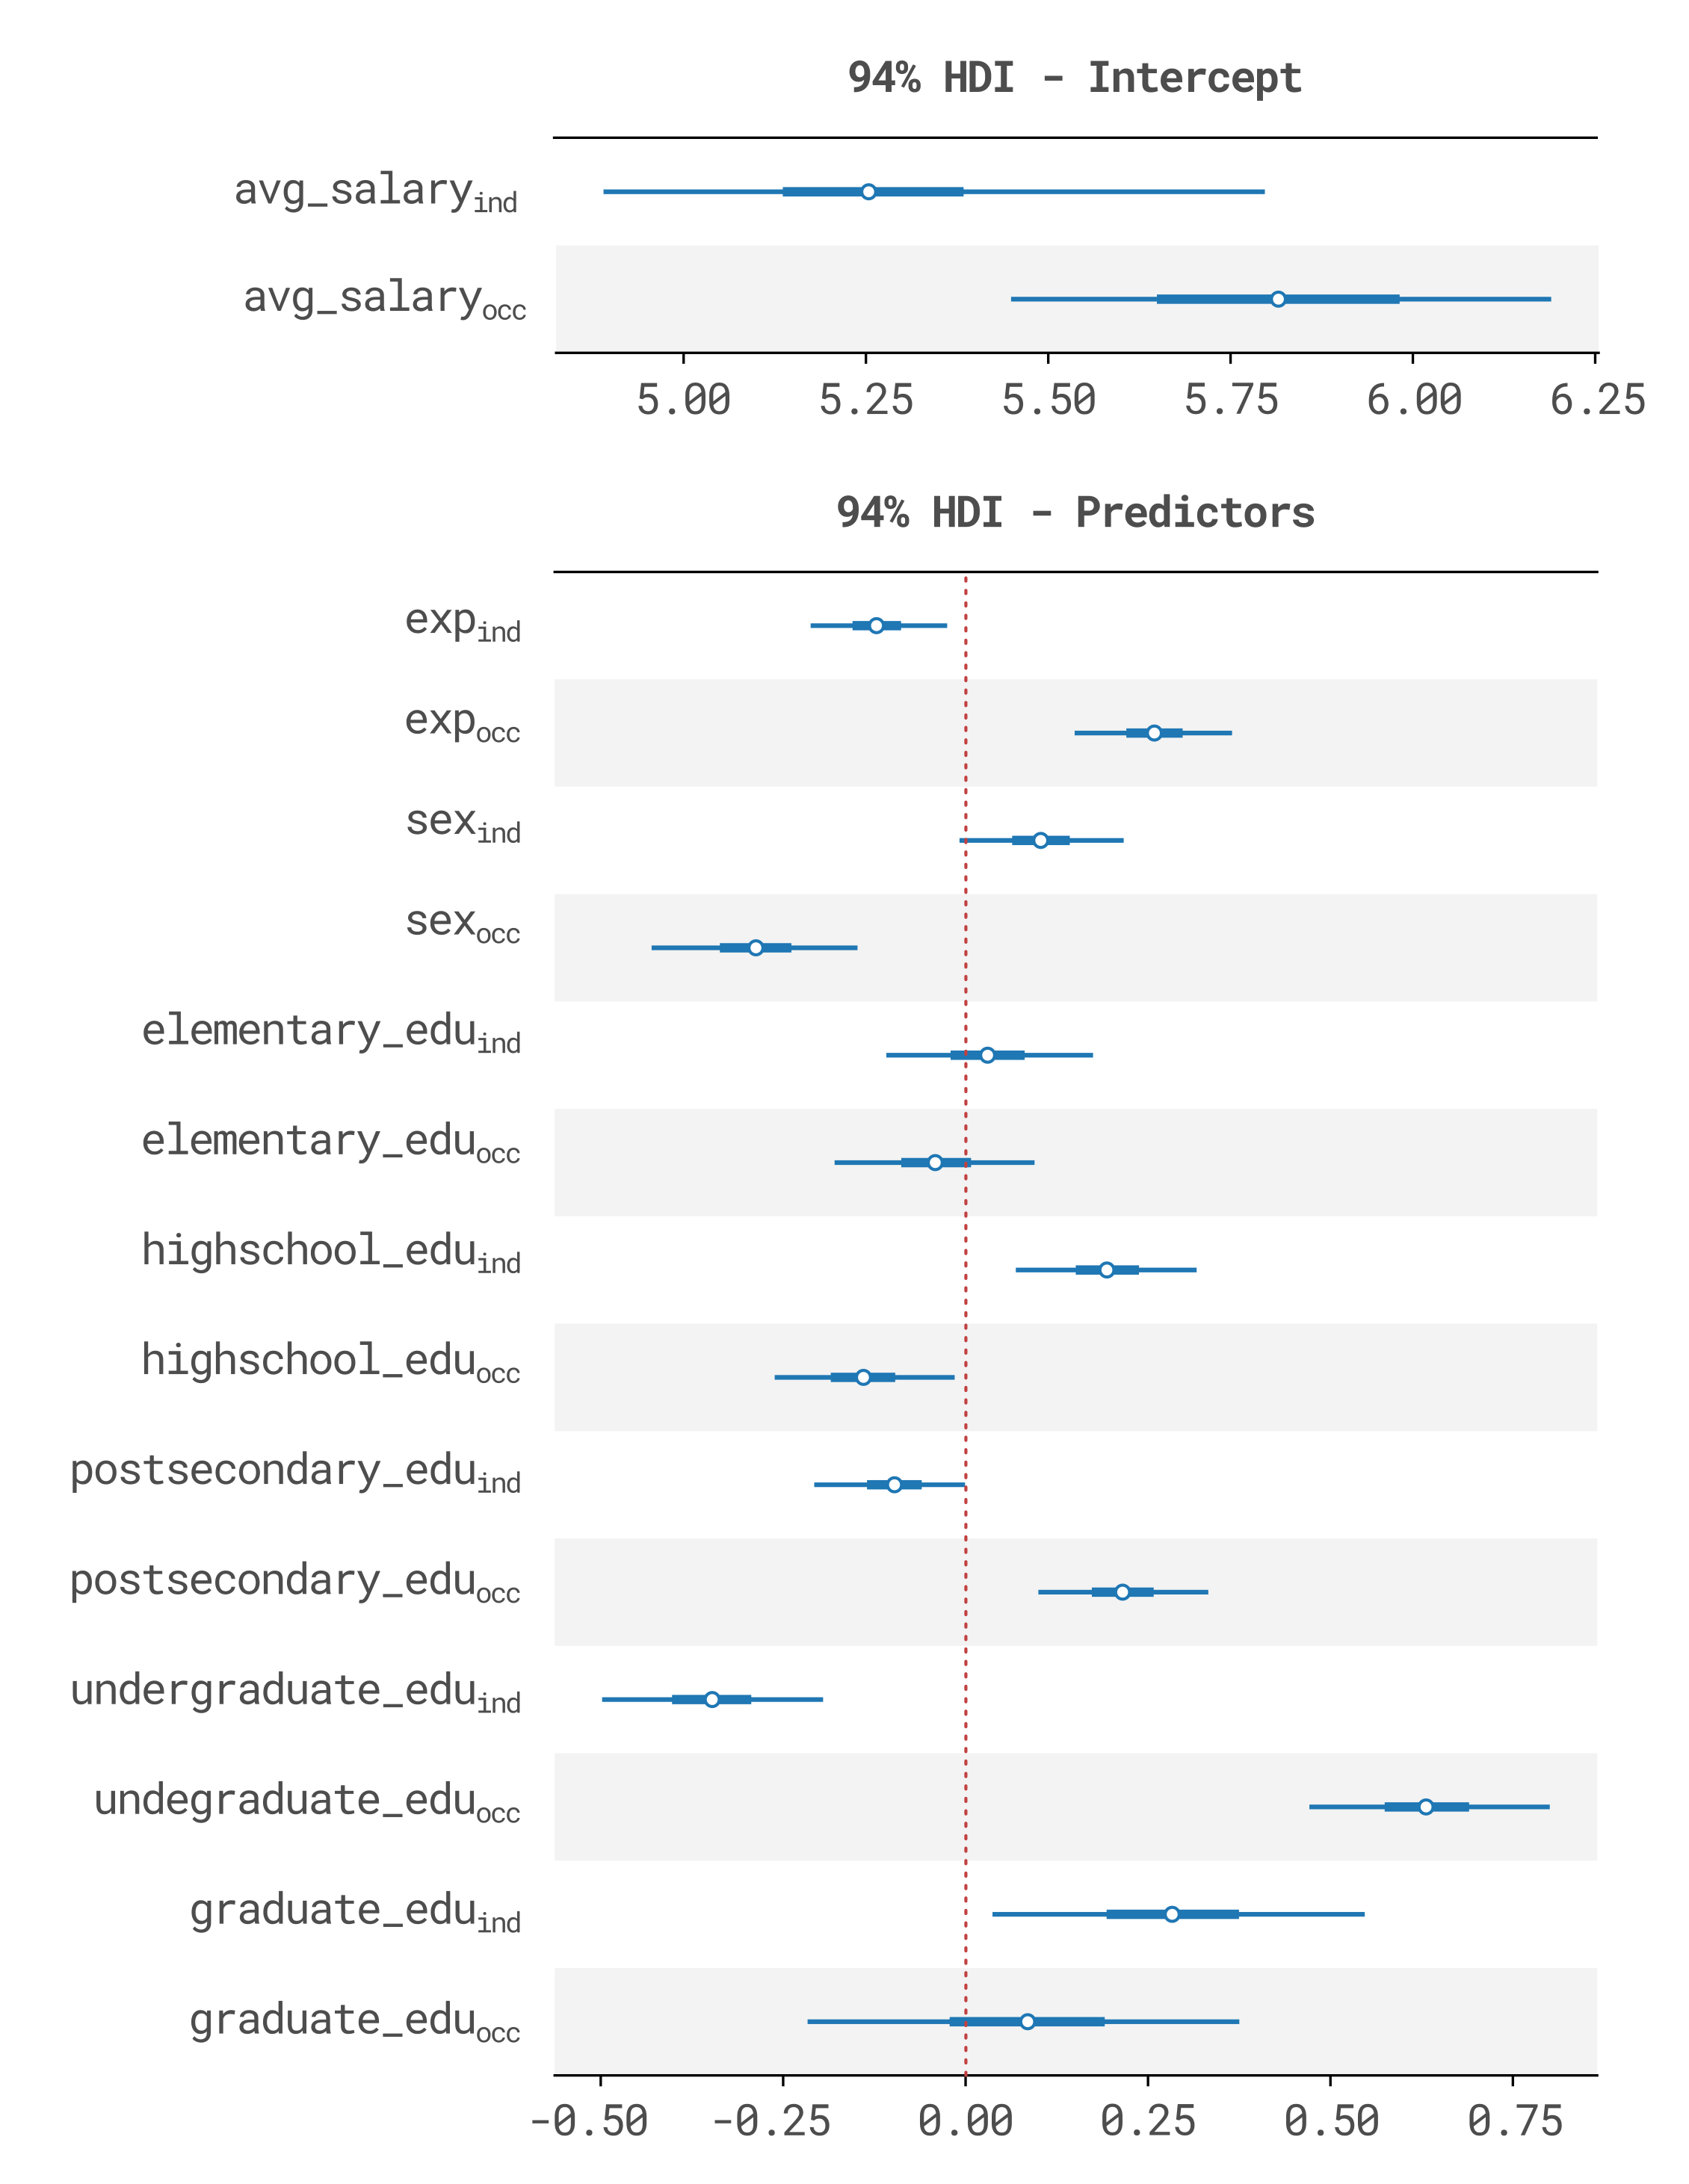
\includegraphics[width=0.6\textwidth]{images/appendix/final.png}
    \caption{Posterior distributions of model parameters for the final model (*All categories aggregated).}
    \label{fig:posterior_dists_final}
\end{figure}


\end{sloppypar}
\end{document}
